\documentclass[10pt]{article}
%\documentclass[14pt]{extarticle}

% Be sure to use PDF Latex
\pdfoutput=1

% links
\usepackage[bookmarks,bookmarksdepth=2, colorlinks=true, linkcolor=blue,citecolor=red, urlcolor=blue]{hyperref}


\usepackage{fullpage}

\usepackage[latin1]{inputenc}
\usepackage{../mystyle}
\usepackage{wrapfig}



\newcommand{\dims}{d}


\graphicspath{{../figures/}}



\title{Course notes on\\Optimization for Machine Learning} 

\author{%
\begin{tabular}{c}
	Gabriel Peyr{\'e} \\ CNRS \& DMA \\
	 \'Ecole Normale Sup\'erieure \\
	 \url{gabriel.peyre@ens.fr}\\
	 \url{https://mathematical-tours.github.io}\\
	 \url{www.numerical-tours.com}
\end{tabular}
}


\date{\today}

%%

\begin{document}

\maketitle

\begin{abstract}
		This document presents first order optimization methods and their applications to machine learning. 
		%
		This is not a course on machine learning (in particular it does not cover modeling and statistical considerations) and it is focussed on the use and analysis of cheap methods that can scale to large datasets and models with lots of parameters. These methods are variations around the notion of ``gradient descent'', so that the computation of gradients plays a major role.
		%
		This course covers basic theoretical properties of optimization problems (in particular convex analysis and first order differential calculus), the gradient descent method, the stochastic gradient method, automatic differentiation, shallow and deep networks.  
\end{abstract}

\tableofcontents

 

% !TEX root = ../optim-ml/OptimML.tex

%%%%%%%%%%%%%%%%%%%%%%%%%%%%%%%%%%%%%%%%%%%%%%%%%%%%%%%%%%%%%%%%%%%%%%%%%%%%%%%%%%
%%%%%%%%%%%%%%%%%%%%%%%%%%%%%%%%%%%%%%%%%%%%%%%%%%%%%%%%%%%%%%%%%%%%%%%%%%%%%%%%%%
%%%%%%%%%%%%%%%%%%%%%%%%%%%%%%%%%%%%%%%%%%%%%%%%%%%%%%%%%%%%%%%%%%%%%%%%%%%%%%%%%%
\section{Motivation in Machine Learning}

%%%%%%%%%%%%%%%%%%%%%%%%%%%%%%%%%%%%%%%%%%%%%%%%%%%%%%%%%%%%%%%%%%%%%%%%%%%%%%%%%%
\subsection{Unconstraint optimization}

In most part of this Chapter, we consider unconstrained convex optimization problems of the form 
\eql{\label{eq-general-pbm} 
	\uinf{x \in \RR^p} f(x),
}
and try to devise ``cheap'' algorithms with a low computational cost per iteration to approximate a minimizer when it exists. 
%
The class of algorithms considered are first order, i.e. they make use of gradient information. In the following, we denote 
\eq{
	\uargmin{x} f(x) \eqdef \enscond{x \in \RR^p}{ f(x) = \inf{f}}, 
} 
to indicate the set of points (it is not necessarily a singleton since the minimizer might be non-unique) that achieve the minimum of the function $f$. One might have $\argmin f = \emptyset$ (this situation is discussed below), but in case a minimizer exists, we denote the optimization problem as
\eql{\label{eq-general-pbm-min} 
	\umin{x \in \RR^p} f(x).
}


In typical learning scenario, $f(x)$ is the empirical risk for regression or classification, and $p$ is the number of parameter. For instance, in the simplest case of linear models, we denote $(a_i,y_i)_{i=1}^n$ where $a_i \in \RR^p$ are the features. 
%
In the following, we denote $A \in \RR^{n \times p}$ the matrix whose rows are the $a_i$.


\begin{figure}
\centering
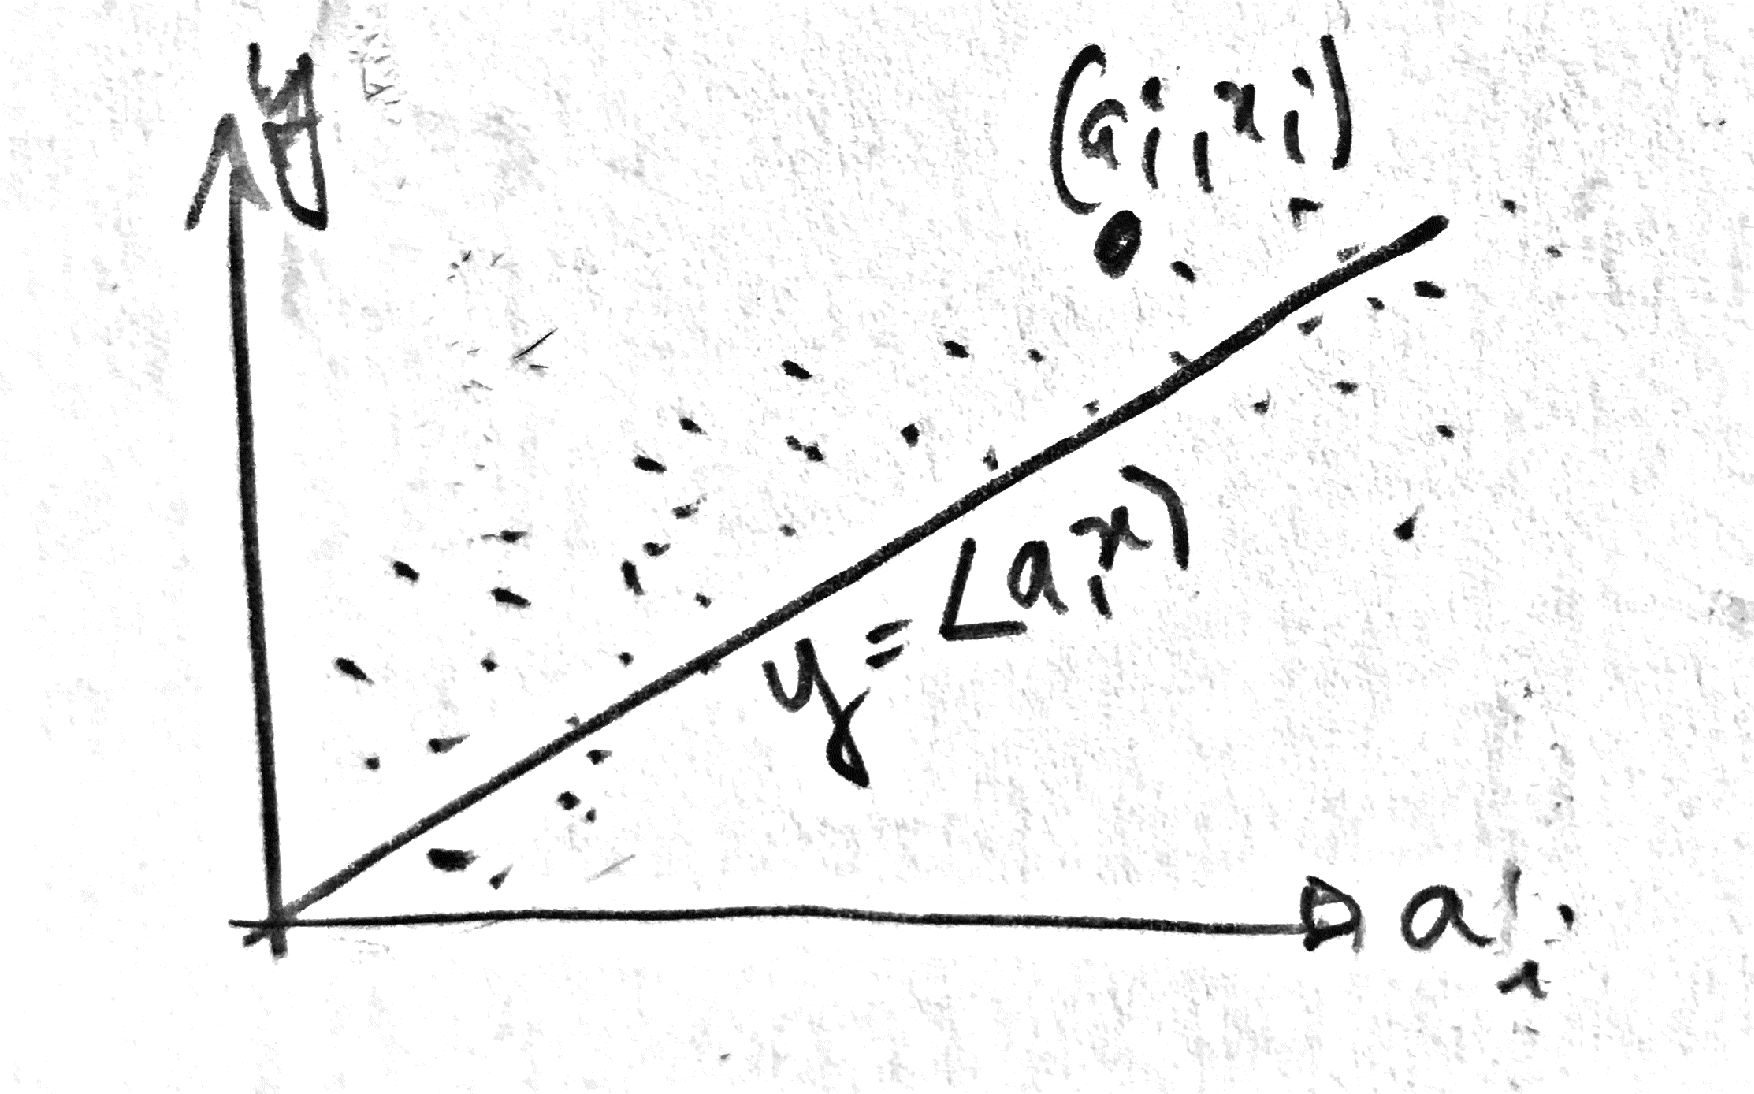
\includegraphics[width=.2\linewidth]{optim-smooth/ml-exemp-1} \quad
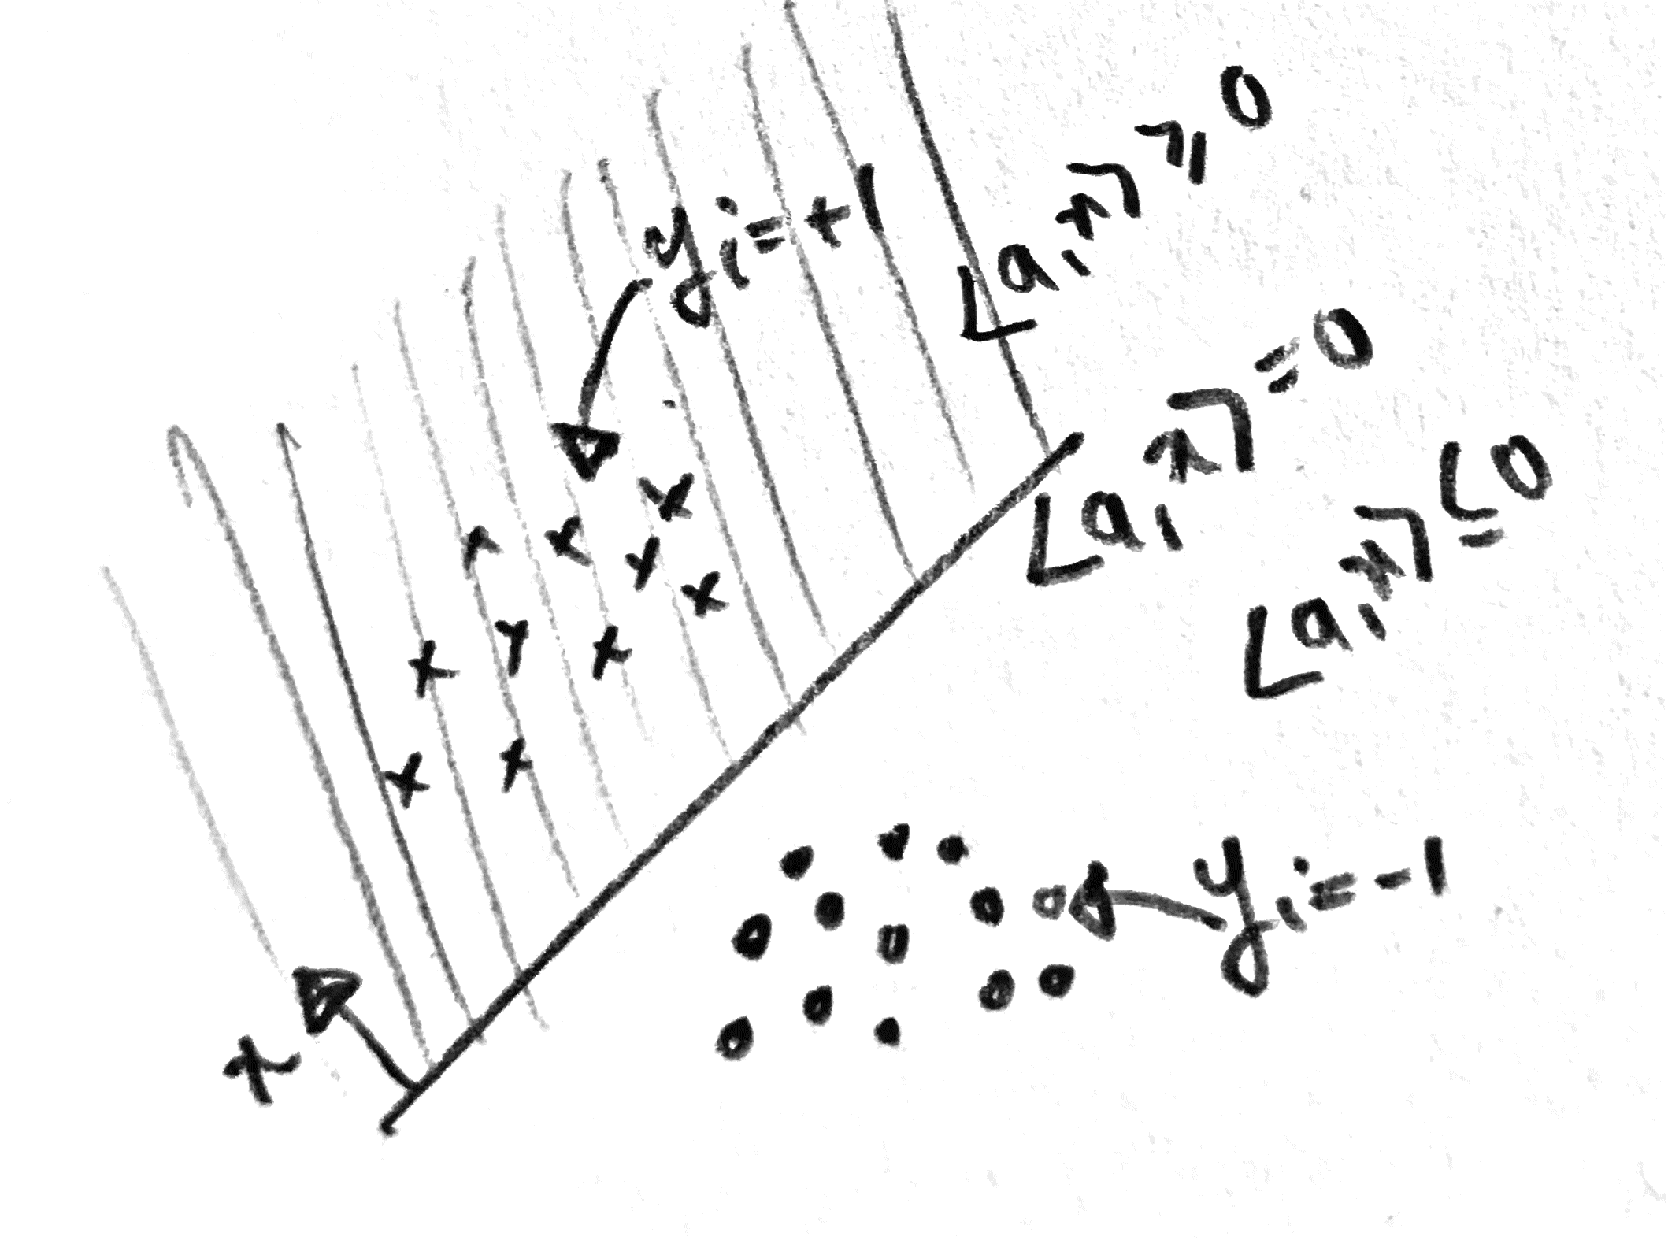
\includegraphics[width=.2\linewidth]{optim-smooth/ml-exemp-2} \quad
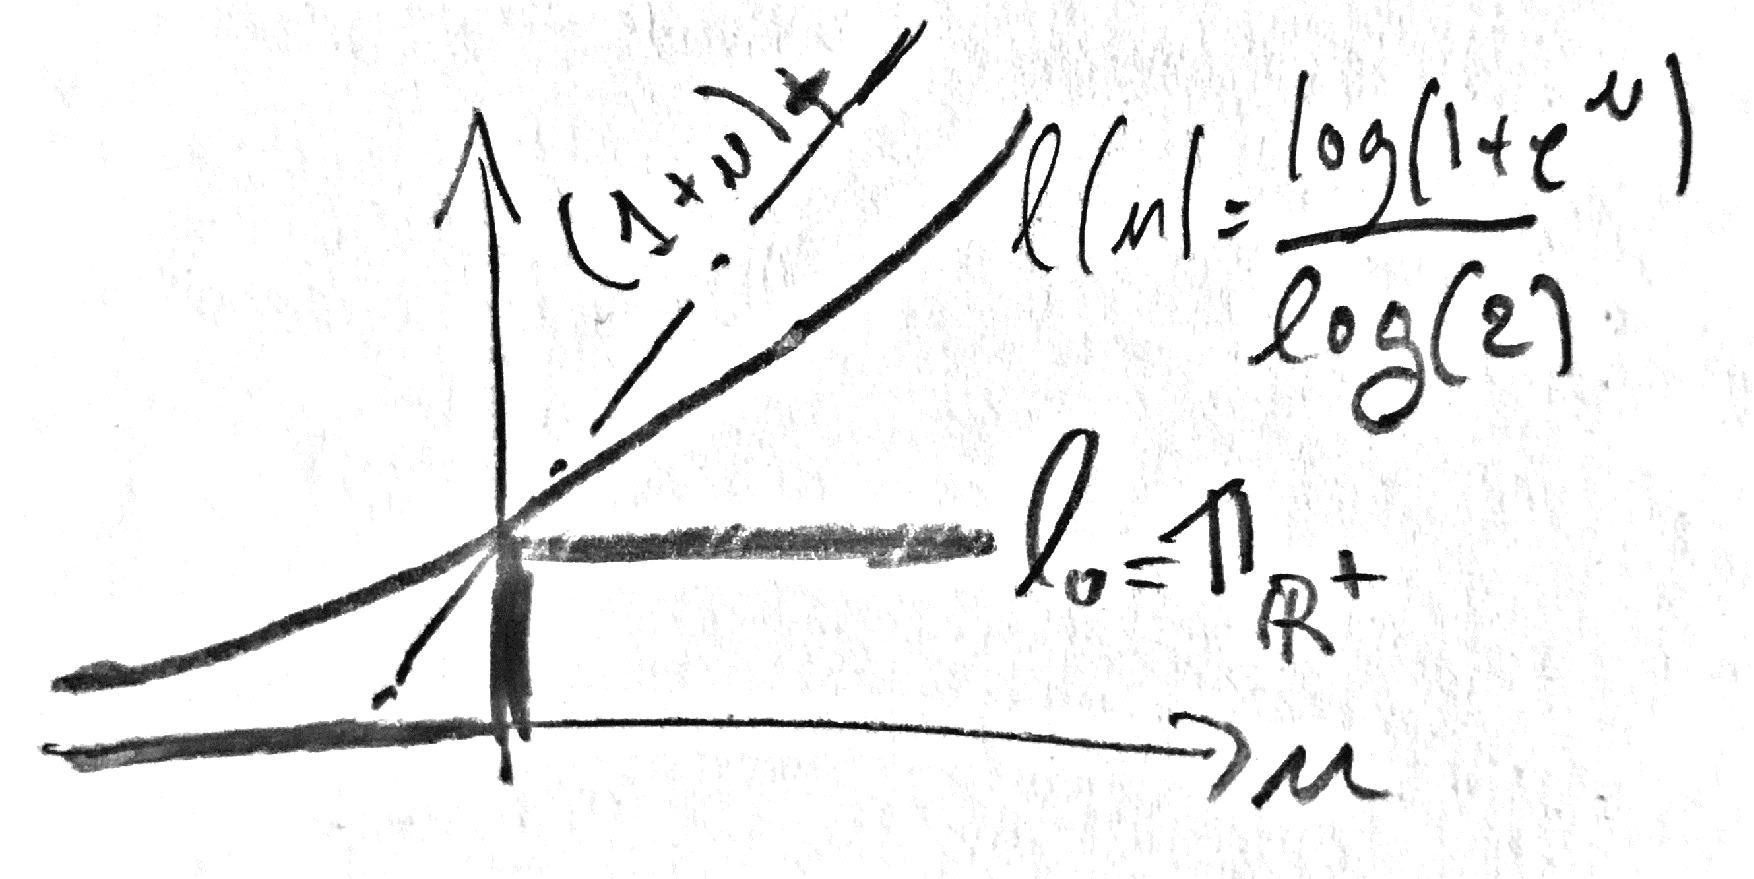
\includegraphics[width=.3\linewidth]{optim-smooth/classif-loss}
\caption{\label{fig-ml-ex}
Left: linear regression, middle: linear classifier, right: loss function for classification.
}
\end{figure}


%%%%%%%%%%%%%%%%%%%%%%%%%%%%%%%%%%%%%%%%%%%%%%%%%%%%%%%%%%%%%%%%%%%%%%%%%%%%%%%%%%
\subsection{Regression}

For regression, $y_i \in \RR$, in which case
\eql{\label{eq-least-square}
	f(x) =  \frac{1}{2}\sum_{i=1}^n (y_i-\dotp{x}{a_i})^2 = \frac{1}{2}\norm{Ax-y}^2, 
} 
is the least square quadratic risk function (see Fig.~\ref{fig-ml-ex}).
%
Here $\dotp{u}{v}=\sum_{i=1}^p u_i v_i$ is the canonical inner product in $\RR^p$ and $\norm{\cdot}^2=\dotp{\cdot}{\cdot}$. 


%%%%%%%%%%%%%%%%%%%%%%%%%%%%%%%%%%%%%%%%%%%%%%%%%%%%%%%%%%%%%%%%%%%%%%%%%%%%%%%%%%
\subsection{Classification}

For classification, $y_i \in \{-1,1\}$, in which case
\eql{\label{eq-classif}
	f(x) = \sum_{i=1}^n \ell(-y_i \dotp{x}{a_i}) = L( - \diag(y) A x )
}
where $\ell$ is a smooth approximation of the 0-1 loss $1_{\RR^+}$.
%
For instance $\ell(u)=\log(1+\exp(u))$, and $\diag(y) \in \RR^{n \times n}$ is the diagonal matrix with $y_i$ along the diagonal (see Fig.~\ref{fig-ml-ex}, right). Here the separable loss function $L = \RR^n \rightarrow \RR$ is, for $z \in \RR^n$, $L(z)=\sum_i \ell(z_i)$. 


%%%%%%%%%%%%%%%%%%%%%%%%%%%%%%%%%%%%%%%%%%%%%%%%%%%%%%%%%%%%%%%%%%%%%%%%%%%%%%%%%%
%%%%%%%%%%%%%%%%%%%%%%%%%%%%%%%%%%%%%%%%%%%%%%%%%%%%%%%%%%%%%%%%%%%%%%%%%%%%%%%%%%
%%%%%%%%%%%%%%%%%%%%%%%%%%%%%%%%%%%%%%%%%%%%%%%%%%%%%%%%%%%%%%%%%%%%%%%%%%%%%%%%%%
\section{Basics of Convex Analysis}

%%%%%%%%%%%%%%%%%%%%%%%%%%%%%%%%%%%%%%%%%%%%%%%%%%%%%%%%%%%%%%%%%%%%%%%%%%%%%%%%%%
\subsection{Existence of Solutions}

In general, there might be no solution to the optimization~\eqref{eq-general-pbm}. This is of course the case if $f$ is unbounded by below, for instance $f(x)=-x^2$ in which case the value of the minimum is $-\infty$. But this might also happen if $f$ does not grow at infinity, for instance $f(x)=e^{-x}$, for which $\min f = 0$ but there is no minimizer.

\begin{figure}
\centering
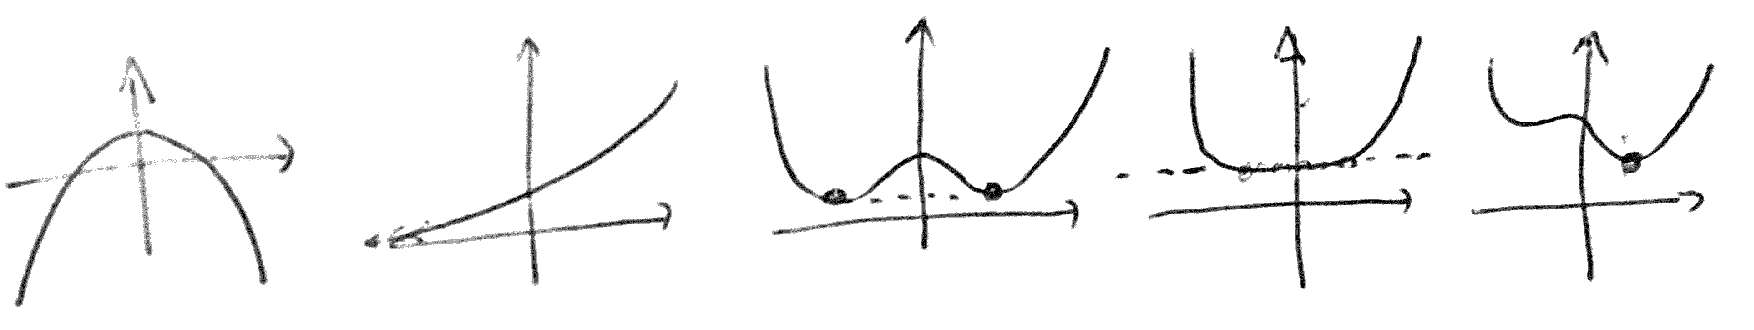
\includegraphics[width=.9\linewidth]{optim-smooth/uniqueness}
\caption{\label{fig-minimizer-exists}
Left: non-existence of minimizer, middle: multiple minimizers, right: uniqueness.
}
\end{figure}

In order to show existence of a minimizer, and that the set of minimizer is bounded (otherwise one can have problems with optimization algorithm that could escape to infinity), one needs to show that one can replace the whole space $\RR^p$ by a compact sub-set $\Om \subset \RR^p$ (i.e. $\Om$ is bounded and close) and that $f$ is continuous on $\Om$ (one can replace this by a weaker condition, that $f$ is lower-semi-continuous, but we ignore this here).  A way to show that one can consider only a bounded set is to show that $f(x) \rightarrow +\infty$ when $x \rightarrow +\infty$. Such a function is called coercive. In this case, one can choose any $x_0 \in \RR^p$ and consider its associated lower-level set
\eq{
	\Om = \enscond{x \in \RR^p}{f(x) \leq f(x_0)}
}
which is bounded because of coercivity, and closed because $f$ is continuous. One can actually show that for convex function, having a bounded set of minimizer is equivalent to the function being coercive (this is not the case for non-convex function, for instance $f(x)=\min(1,x^2)$ has a single minimum but is not coercive). 

\begin{figure}
\centering
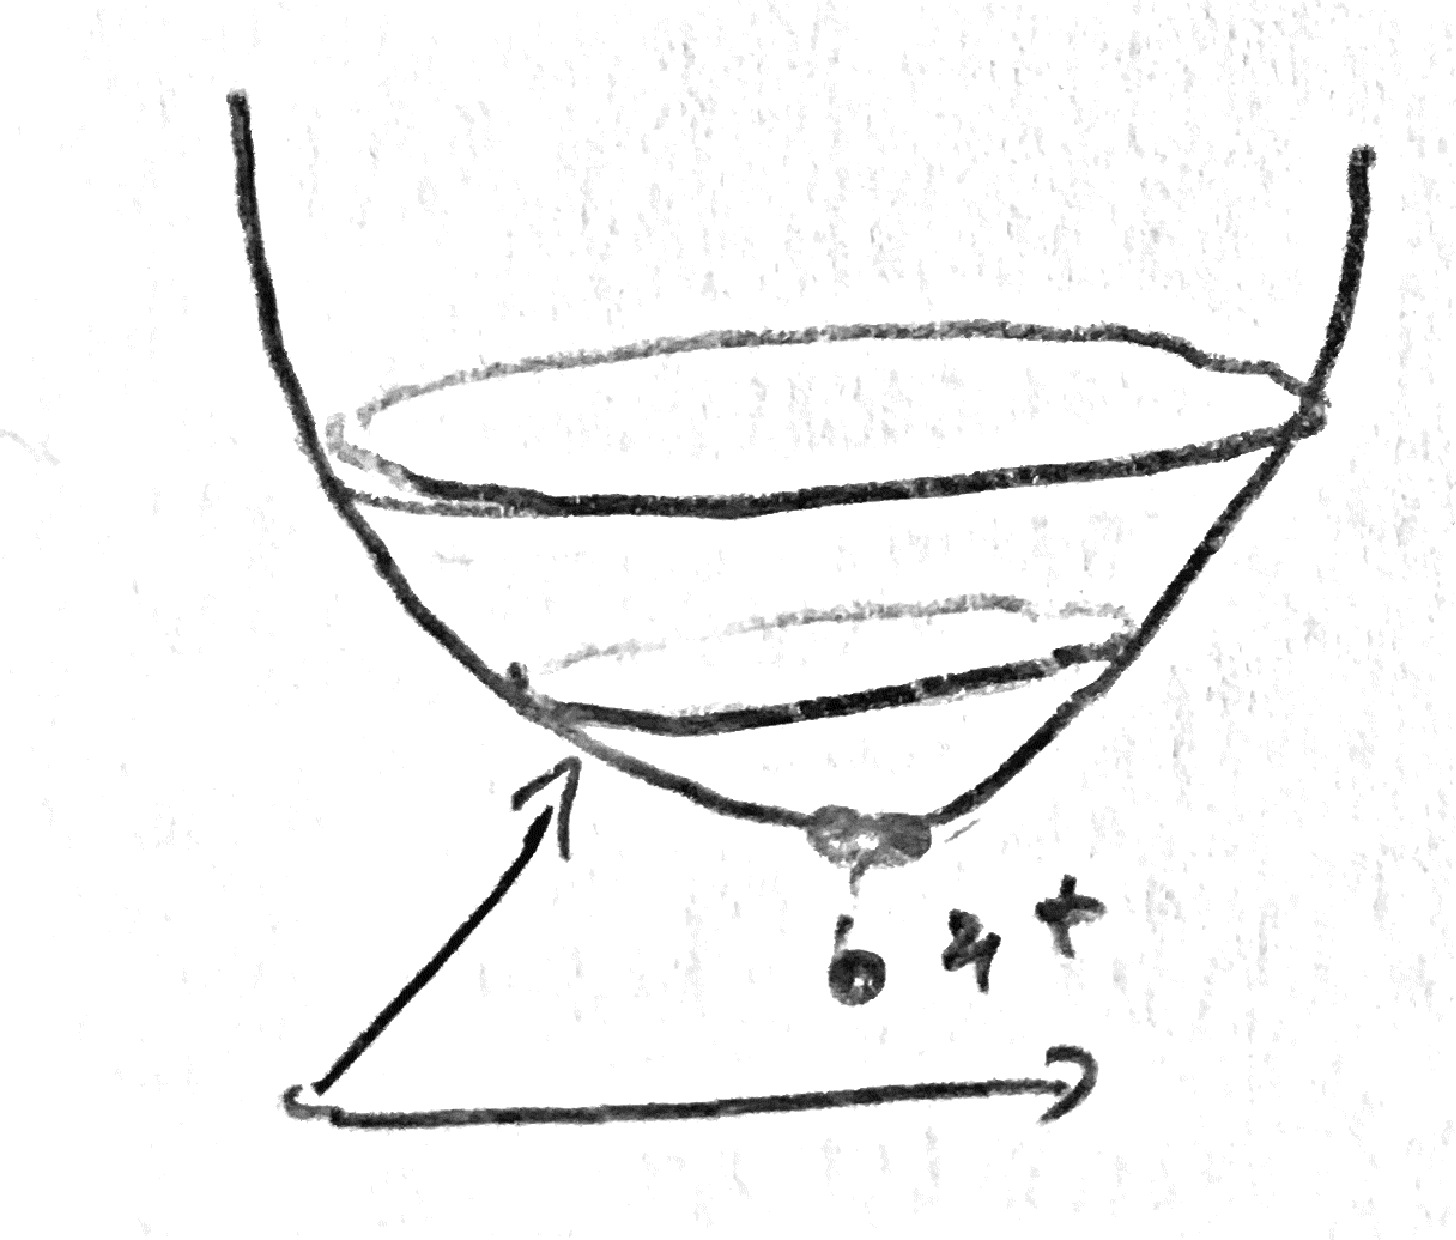
\includegraphics[width=.2\linewidth]{optim-smooth/least-square-1} \quad
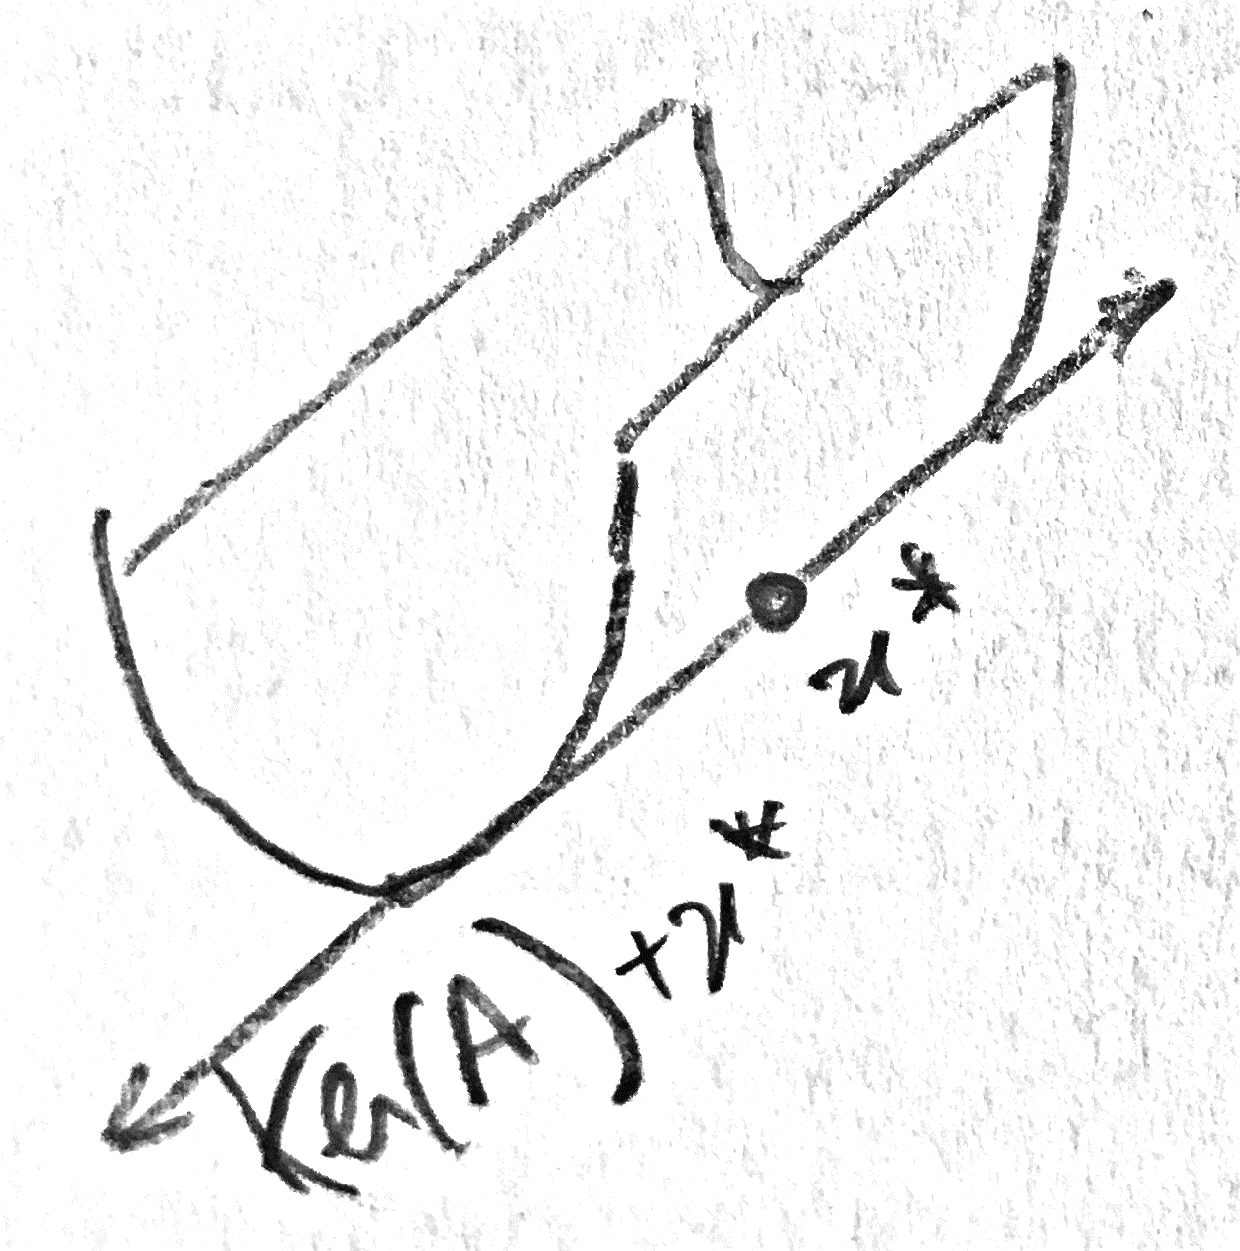
\includegraphics[width=.2\linewidth]{optim-smooth/least-square-2} 
\caption{\label{fig-least-square}
Coercivity condition for least squares.
}
\end{figure}

\begin{exmp}[Least squares]
For instance, for the quadratic loss function $f(x)=\frac{1}{2}\norm{Ax-y}^2$, coercivity holds if and only if $\ker(A)=\{0\}$ (this corresponds to the overdetermined setting). Indeed, if $\ker(A) \neq \{0\}$ if $x^\star$ is a solution, then $x^\star+u$ is also solution for any $u \in \ker(A)$, so that the set of minimizer is unbounded.
%
On contrary, if $\ker(A) = \{0\}$, we will show later that the set of minimizer is unique, see Fig.~\ref{fig-least-square}. 
%
If $\ell$ is strictly convex, the same conclusion holds in the case of classification.
\end{exmp}

%%%%%%%%%%%%%%%%%%%%%%%%%%%%%%%%%%%%%%%%%%%%%%%%%%%%%%%%%%%%%%%%%%%%%%%%%%%%%%%%%%
\subsection{Convexity}

Convex functions define the main class of functions which are somehow ``simple'' to optimize, in the sense that all minimizers are global minimizers, and that there are often efficient methods to find these minimizers (at least for smooth convex functions). A convex function is such that for any pair of point $(x,y) \in (\RR^p)^2$, 
\eql{\label{eq-convexity-def}
	\foralls t \in [0,1], \quad
		f((1-t)x + t y) \leq (1-t)f(x) + t f(y)
}
which means that the function is below its secant (and actually also above its tangent when this is well defined), see Fig.~\ref{fig-cvx-vs-noncvx}. 
%
If $x^\star$ is a local minimizer of a convex $f$, then $x^\star$ is a global minimizer, i.e. $x^\star \in \argmin f$.  


Convex function are very convenient because they are stable under lots of transformation. In particular, if $f$, $g$ are convex and $a, b$ are positive, $a f + b g$ is convex (the set of convex function is itself an infinite dimensional convex cone!) and so is $\max(f,g)$. If $g : \RR^q \rightarrow \RR$ is convex and $B \in \RR^{q \times p}, b \in \RR^q$ then $f(x) = g(B x+b)$ is convex. 
%
This shows immediately that the square loss appearing in~\eqref{eq-least-square} is convex, since $\norm{\cdot}^2/2$ is convex (as a sum of squares). 
%
Also, similarly, if $\ell$ and hence $L$ is convex, then the classification loss function~\eqref{eq-classif} is itself convex. 

\begin{figure}
\centering
\begin{tabular}{cccc}
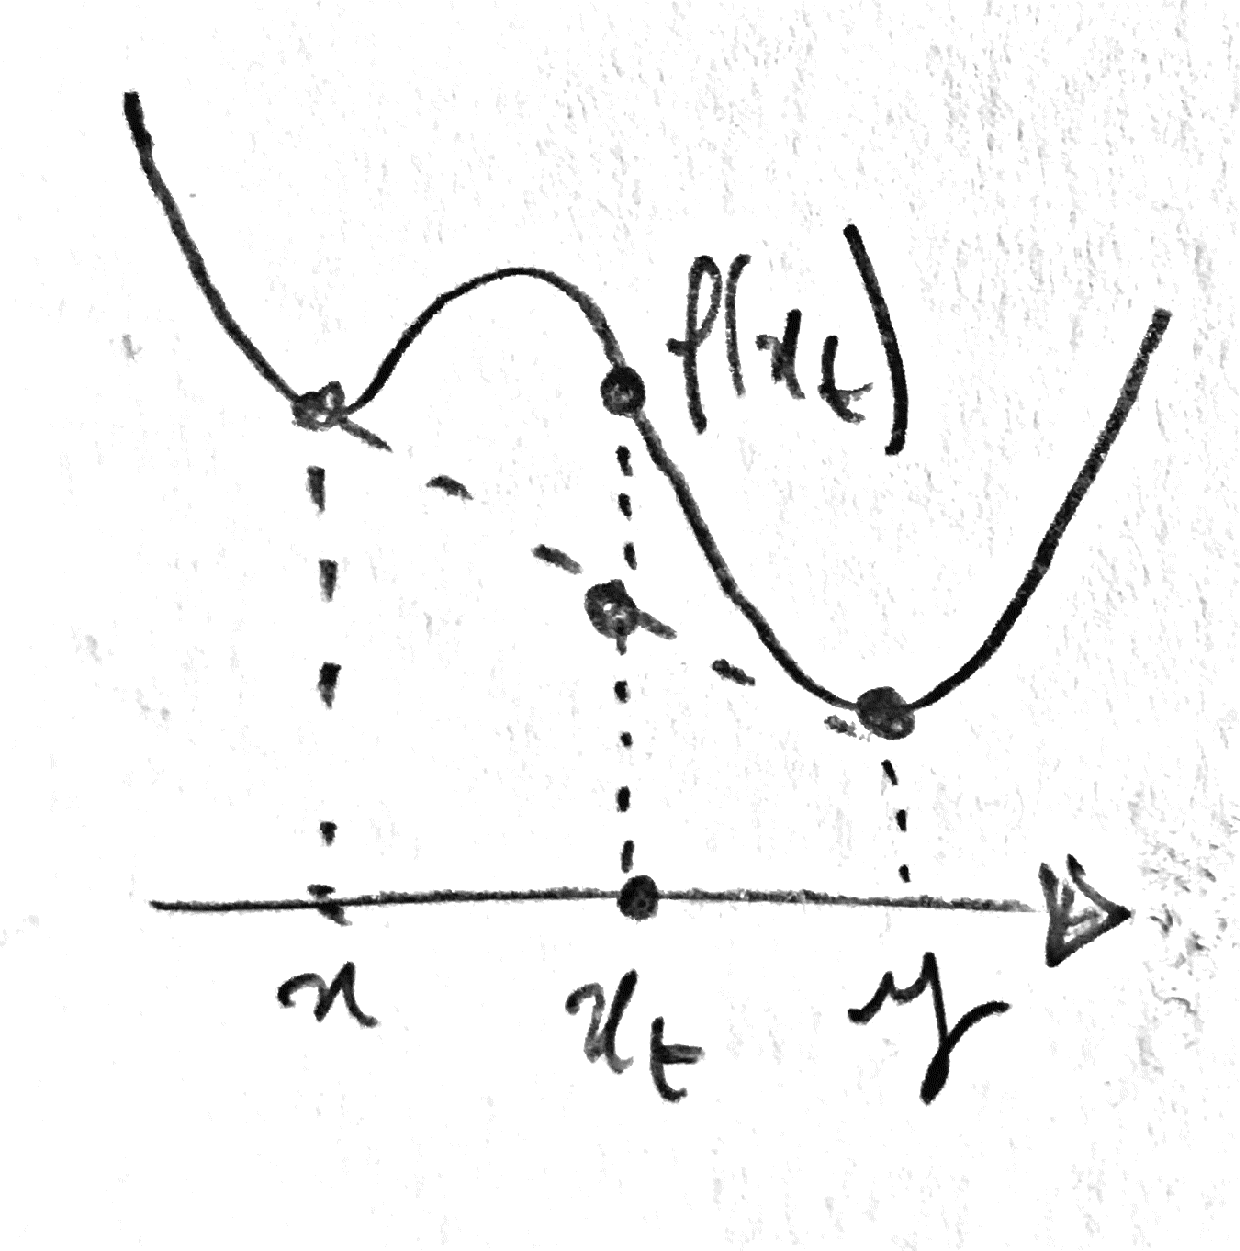
\includegraphics[width=.2\linewidth]{optim-smooth/cvx-vs-noncvx-1} &
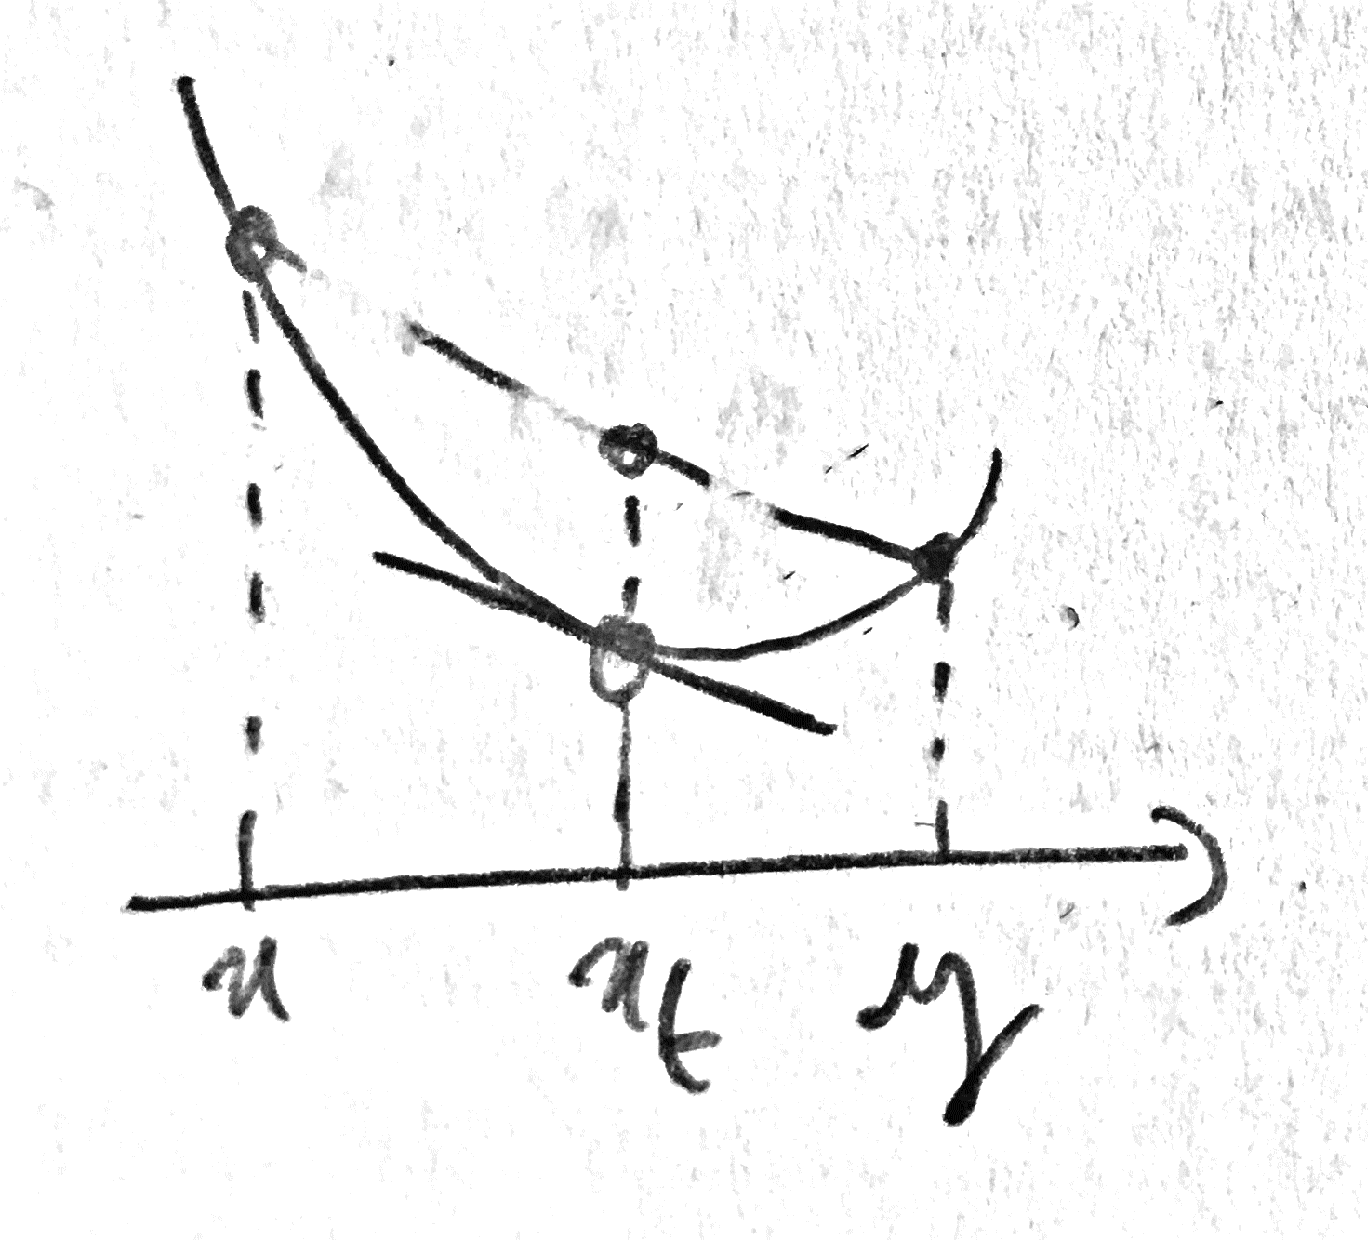
\includegraphics[width=.2\linewidth]{optim-smooth/cvx-vs-noncvx-2} &
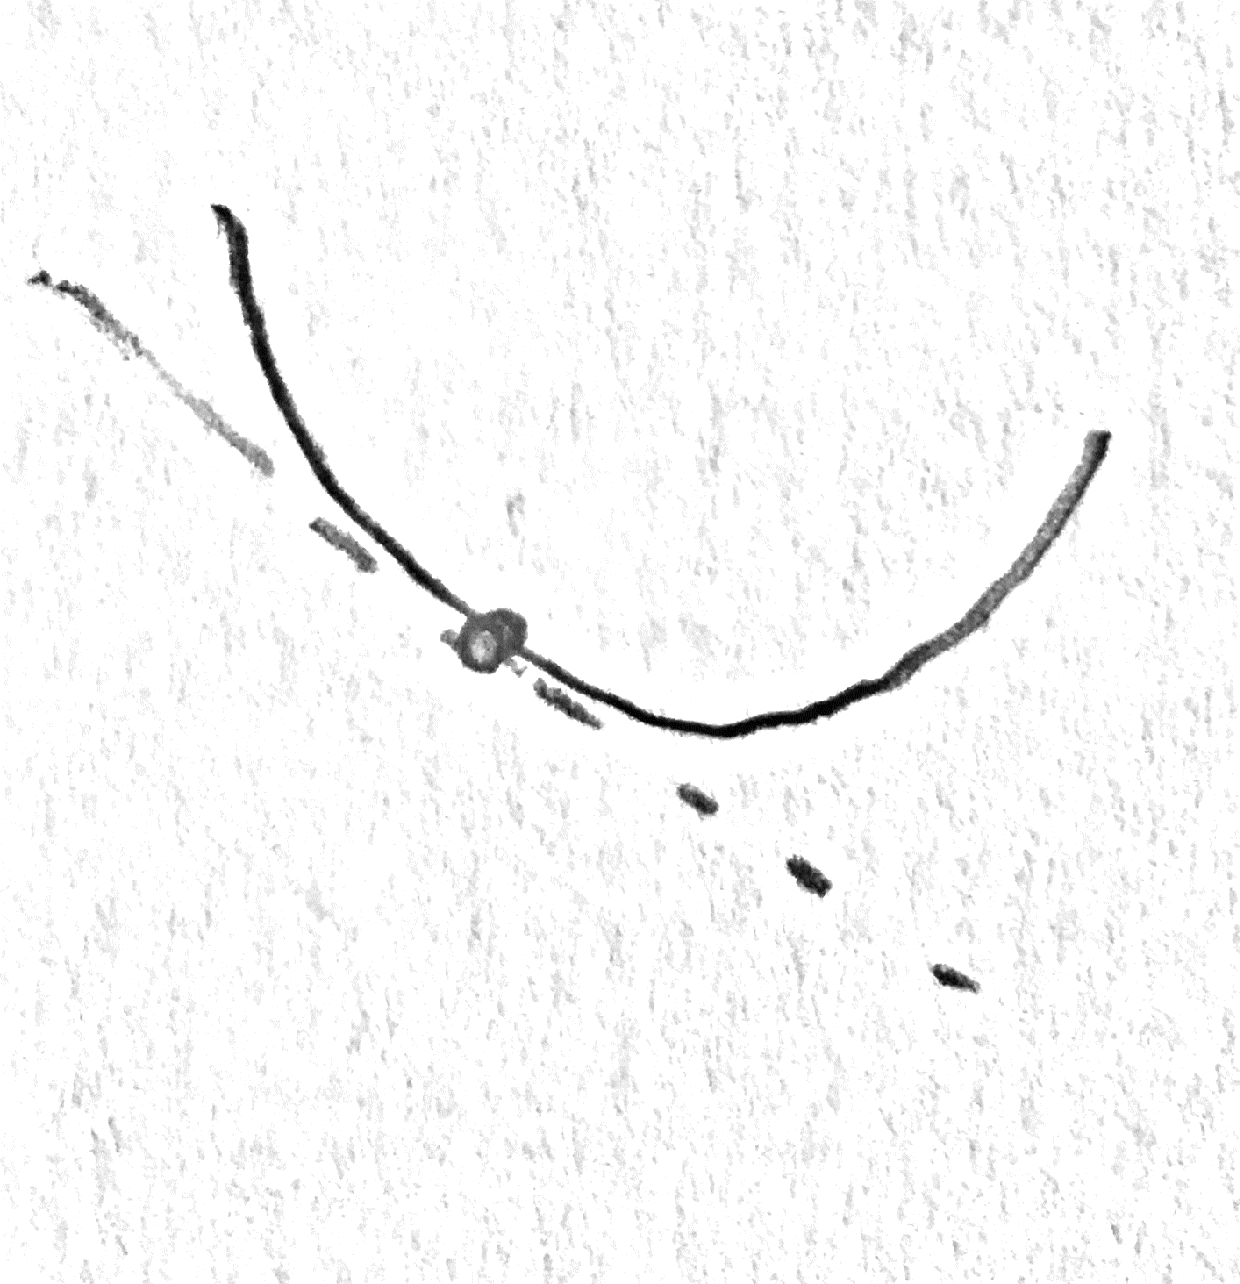
\includegraphics[width=.2\linewidth]{optim-smooth/strictly-cvx-2} &
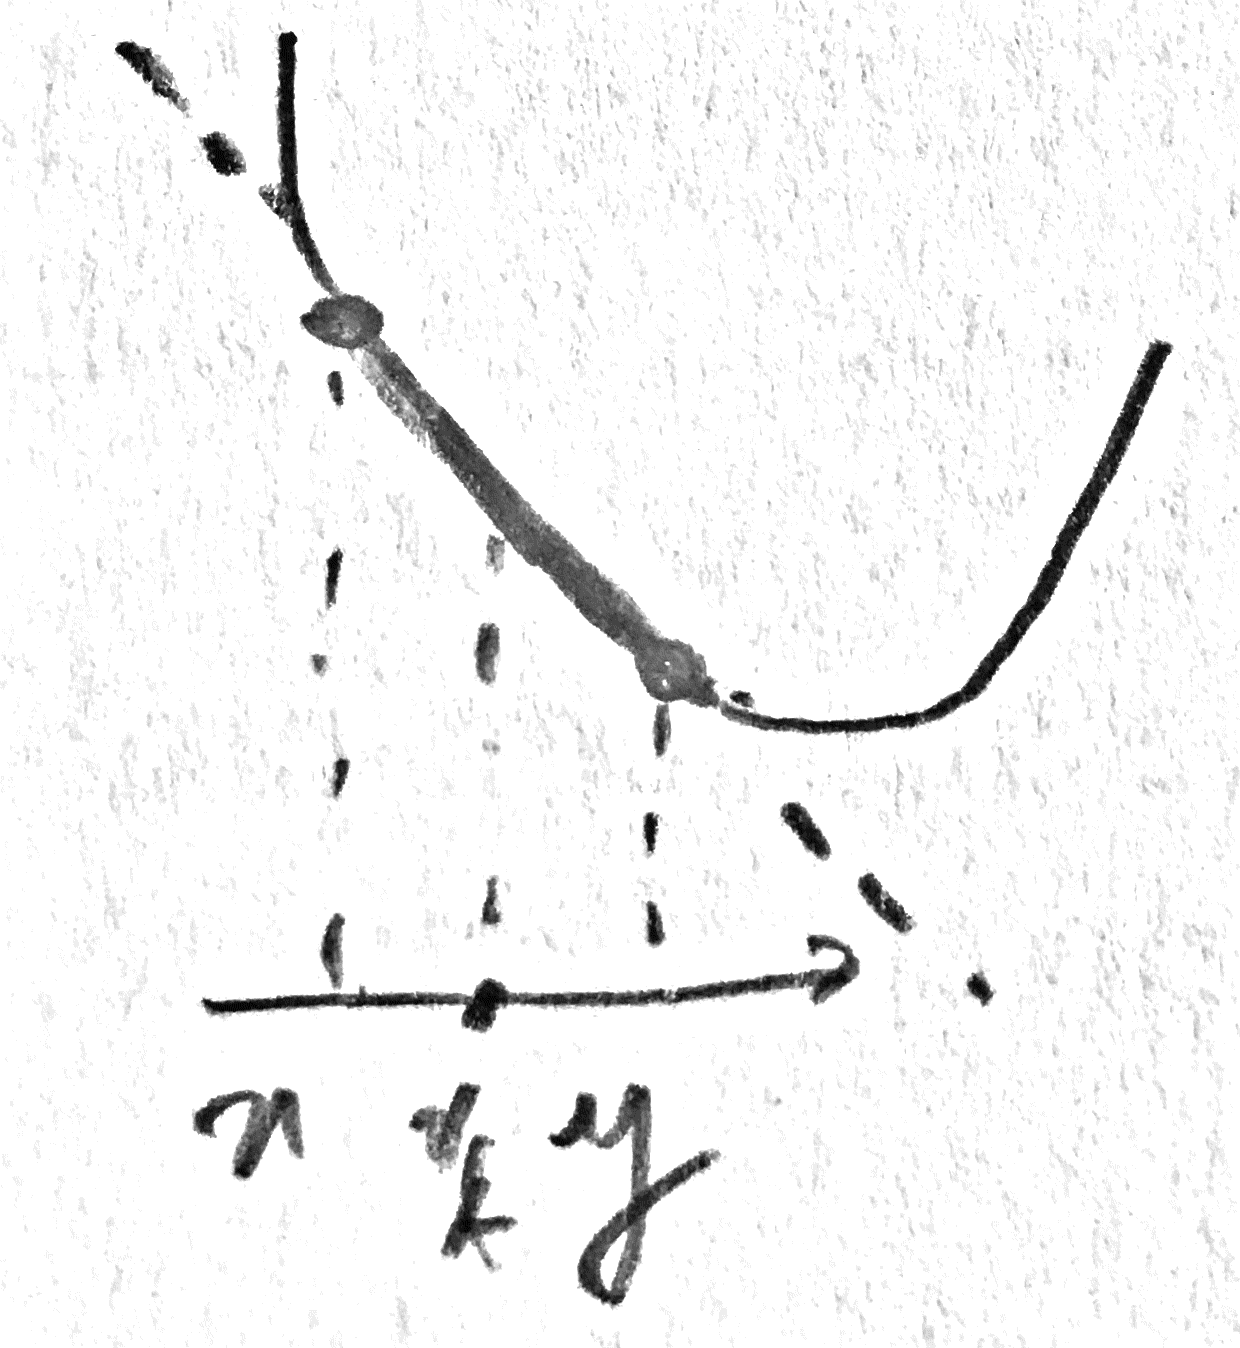
\includegraphics[width=.15\linewidth]{optim-smooth/strictly-cvx-1} 
\end{tabular}
\caption{\label{fig-cvx-vs-noncvx}
Convex vs. non-convex functions ; Strictly convex vs. non strictly convex functions.
}
\end{figure}



\begin{figure}
\centering
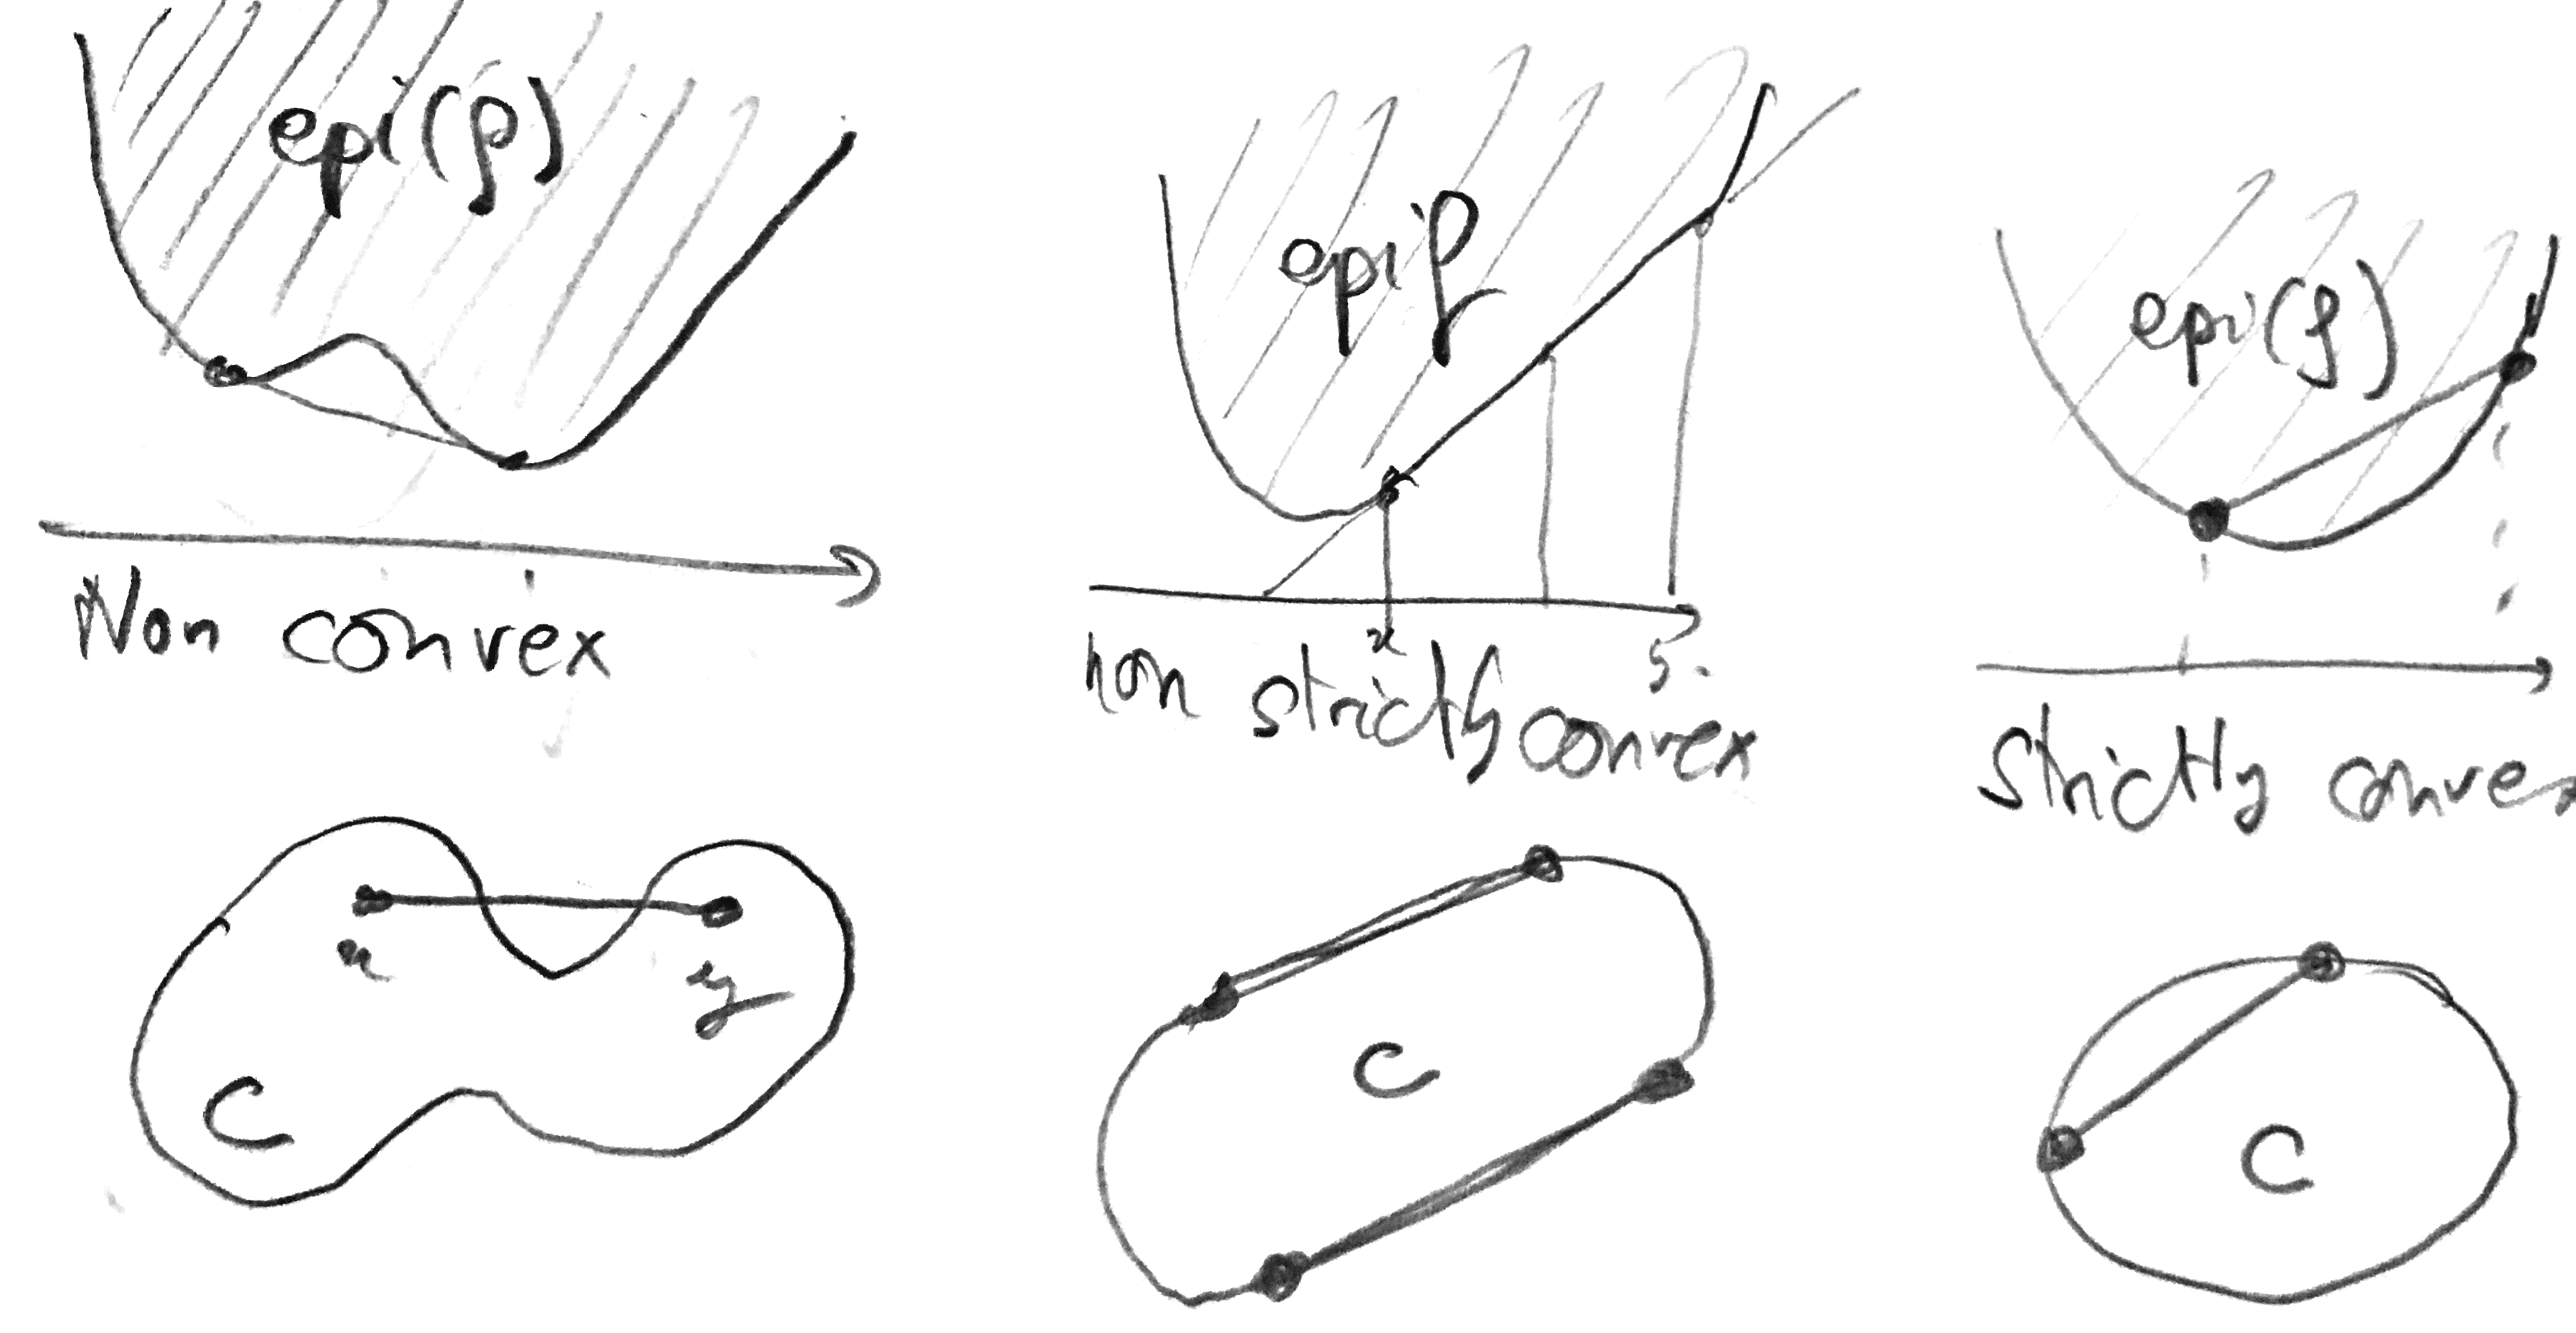
\includegraphics[width=.6\linewidth]{optim-smooth/convex-examples.png} 
\caption{\label{fig-cvx-set}
Comparison of convex functions $f : \RR^p \rightarrow \RR$ (for $p=1$) and convex sets $C \subset \RR^p$ (for $p=2$).
}
\end{figure}

%%%
\paragraph{Strict convexity.}

When $f$ is convex, one can strengthen the condition~\eqref{eq-convexity-def} and impose that the inequality is strict for $t \in ]0,1[$ (see Fig.~\ref{fig-cvx-vs-noncvx}, right), i.e.
\eql{\label{eq-strict-convexity-def}
	\foralls t \in ]0,1[, \quad
		f((1-t)x + t y) < (1-t)f(x) + t f(y).
}
In this case, if a minimum $x^\star$ exists, then it is unique.  Indeed, if $x_1^\star \neq x_2^\star$ were two different minimizer, one would have by strict convexity $f(\frac{x_1^\star+x_2^\star}{2}) < f(x_1^\star)$ which is impossible.

\begin{exmp}[Least squares]
	For the quadratic loss function $f(x)=\frac{1}{2}\norm{Ax-y}^2$, strict convexity is equivalent to $\ker(A)=\{0\}$.
	Indeed, we see later that its second derivative is $\partial^2 f(x)=A^\top A$ and that strict convexity is implied by the eigenvalues of $A^\top A$ being strictly positive. The eigenvalues of $A^\top A$ being positive, it is equivalent to $\ker(A^\top A)=\{0\}$ (no vanishing eigenvalue), and $A^\top A z = 0$ implies $\dotp{A^\top A z}{z}=\norm{Az}^2=0$ i.e. $z \in \ker(A)$.
\end{exmp}

%%%%%%%%%%%%%%%%%%%%%%%%%%%%%%%%%%%%%%%%%%%%%%%%%%%%%%%%%%%%%%%%%%%%%%%%%%%%%%%%%%
\subsection{Convex Sets}

A set $\Om \subset \RR^p$ is said to be convex if for any $(x,y) \in \Om^2$, $(1-t)x + t y \in \Om$ for $t \in [0,1]$.
%
The connexion between convex function and convex sets is that a function $f$ is convex if and only if its epigraph $\text{epi}(f) \eqdef \enscond{(x,t) \in \RR^{p+1}}{t \geq f(x)}$ is a convex set. 

\begin{rem}[Convexity of the set of minimizers]
In general, minimizers $x^\star$ might be non-unique, as shown on Figure~\ref{fig-least-square}. 
%
When $f$ is convex, the set $\argmin(f)$ of minimizers is itself a convex set. 
%
Indeed, if $x_1^\star$ and $x_2^\star$ are minimizers, so that in particular $f(x_1^\star)=f(x_2^\star)=\min(f)$, then $f( (1-t)x_1^\star + t x_2^\star ) \leq (1-t) f(x_1^\star) + t f(x_2^\star) = f(x_1^\star) = \min(f)$, so that $(1-t)x_1^\star + t x_2^\star$ is itself a minimizer. Figure~\ref{fig-cvx-set} shows convex and non-convex sets. 
\end{rem}



%%%%%%%%%%%%%%%%%%%%%%%%%%%%%%%%%%%%%%%%%%%%%%%%%%%%%%%%%%%%%%%%%%%%%%%%%%%%%%%%%%
%%%%%%%%%%%%%%%%%%%%%%%%%%%%%%%%%%%%%%%%%%%%%%%%%%%%%%%%%%%%%%%%%%%%%%%%%%%%%%%%%%
%%%%%%%%%%%%%%%%%%%%%%%%%%%%%%%%%%%%%%%%%%%%%%%%%%%%%%%%%%%%%%%%%%%%%%%%%%%%%%%%%%
\section{Derivative and gradient}

%%%%%%%%%%%%%%%%%%%%%%%%%%%%%%%%%%%%%%%%%%%%%%%%%%%%%%%%%%%%%%%%%%%%%%%%%%%%%%%%%%
\subsection{Gradient}


\wrapfSimple{optim-smooth/gradient-vector-field}
If $f$ is differentiable along each axis, we denote 
\eq{
	\nabla f(x) \eqdef \pa{\pd{f(x)}{x_1}, \ldots,\pd{f(x)}{x_p}}^\top \in \RR^p
}
the gradient vector, so that $\nabla f : \RR^p \rightarrow \RR^p$ is a vector field. Here the partial derivative (when they exits) are defined as
\eq{
	\pd{f(x)}{x_k} \eqdef \lim_{\eta \rightarrow 0} \frac{f(x+\eta \de_k)-f(x)}{\eta} 
}
where $\de_k=(0,\ldots,0,1,0,\ldots,0)^\top \in \RR^p$ is the $k^{\text{th}}$ canonical basis vector.  

Beware that $\nabla f(x)$ can exist without $f$ being differentiable. Differentiability of $f$ at each reads
\eql{\label{eq-grad-dfn}
	f(x+\epsilon) = f(x) + \dotp{\epsilon}{\nabla f(x)} + o(\norm{\epsilon}).
} 
%
Here $R(\epsilon) = o(\norm{\epsilon})$ denotes a quantity which decays faster than $\epsilon$ toward $0$, i.e. $\frac{R(\epsilon)}{\norm{\epsilon}} \rightarrow 0$ as $\epsilon \rightarrow 0$. Existence of partial derivative corresponds to $f$ being differentiable along the axes, while differentiability should hold for any converging sequence of $\epsilon\rightarrow 0$ (i.e. not along along a fixed direction). 
%
A counter example in 2-D is $f(x)=\frac{2 x_1 x_2 (x_1+x_2)}{x_1^2+x_2^2}$ with $f(0)=0$, which is affine with different slope along each radial lines.

Also, $\nabla f(x)$ is the only vector such that the relation~\eqref{eq-grad-dfn}. This means that a possible strategy to both prove that $f$ is differentiable and to obtain a formula for $\nabla f(x)$ is to show a relation of the form 
\eq{
	f(x+\epsilon) = f(x) + \dotp{\epsilon}{g} + o(\norm{\epsilon}), 
}
in which case one necessarily has $\nabla f(x)=g$. 

The following proposition shows that convexity is equivalent to the graph of the function being above its tangents.

\begin{prop}\label{prop-above-tgt}
	If $f$ is differentiable, then
	\eq{
		f \text{ convex} 
		\quad\Leftrightarrow\quad
		\forall (x,x'), \: f(x) \geq f(x') + \dotp{\nabla f(x')}{x-x'}.
	}
\end{prop}
\begin{proof}
	One can write the convexity condition as
	\eq{
		f((1-t)x+tx') \leq (1-t) f(x) + t f(x')
		\qarrq
		\frac{ f( x + t (x'-x) ) - f(x) }{t} \leq f(x')-f(x)
	}
	hence, taking the limit $t \rightarrow 0$ one obtains
	\eq{
		\dotp{\nabla f(x)}{x'-x} \leq f(x')-f(x).
	}
	For the other implication, we apply the right condition replacing $(x,x')$ by $(x, x_t \eqdef (1-t)x+t x')$
	and $(x', (1-t)x+t x')$
	\begin{align*}
		f(x)  & \geq f(x_t) + \dotp{\nabla f(x_t)}{x-x_t} = f(x_t) - t \dotp{\nabla f(x_t)}{x-x'} \\
		f(x') & \geq f(x_t) + \dotp{\nabla f(x_t)}{x'-x_t} = f(x_t) + (1-t) \dotp{\nabla f(x_t)}{x-x'}, 
	\end{align*}
	multiplying these inequality by respectively $1-t$ and $t$, and summing them, gives
	\eq{
		(1-t)f(x)+t f(x') \geq f(x_t).
	}
\end{proof}


%%%%%%%%%%%%%%%%%%%%%%%%%%%%%%%%%%%%%%%%%%%%%%%%%%%%%%%%%%%%%%%%%%%%%%%%%%%%%%%%%%
\subsection{First Order Conditions}

The main theoretical interest (we will see later that it also have algorithmic interest) of the gradient vector is that it is a necessarily condition for optimality, as stated below. 

\begin{prop}\label{prop-cs-min} 
If $x^\star$ is a local minimum of the function $f$ (i.e. that $f(x^\star) \leq f(x)$ for all $x$ in some ball around $x^\star$) then 
\eq{
	\nabla f(x^\star) = 0. 
} 
\end{prop}
\begin{proof}
One has for $\epsilon$ small enough and $u$ fixed 
\eq{
	f(x^\star) \leq f(x^\star+\epsilon u) = f(x^\star) + \epsilon \dotp{\nabla f(x^\star)}{u} + o(\epsilon) 
	\qarrq
	\dotp{\nabla f(x^\star)}{u} \geq o(1)
	\qarrq
	\dotp{\nabla f(x^\star)}{u} \geq 0.
}	
So applying this for $u$ and $-u$ in the previous equation shows that $\dotp{\nabla f(x^\star)}{u}=0$ for all $u$, and hence $\nabla f(x^\star)=0$.
\end{proof}

Note that the converse is not true in general, since one might have $\nabla f(x)=0$ but $x$ is not a local mininimum. For instance $x=0$ for $f(x)=-x^2$ (here $x$ is a maximizer) or $f(x)=x^3$ (here $x$ is neither a maximizer or a minimizer, it is a saddle point), see Fig.~\ref{fig-first-order}. 
%
Note however that in practice, if $\nabla f(x^\star) = 0$ but $x$ is not a local minimum, then $x^\star$ tends to be an unstable equilibrium. Thus most often a gradient-based algorithm will converge to points with $\nabla f(x^\star) = 0$ that are local minimizers.
%
The following proposition shows that a much strong result holds if $f$ is convex.

\begin{figure}
\centering
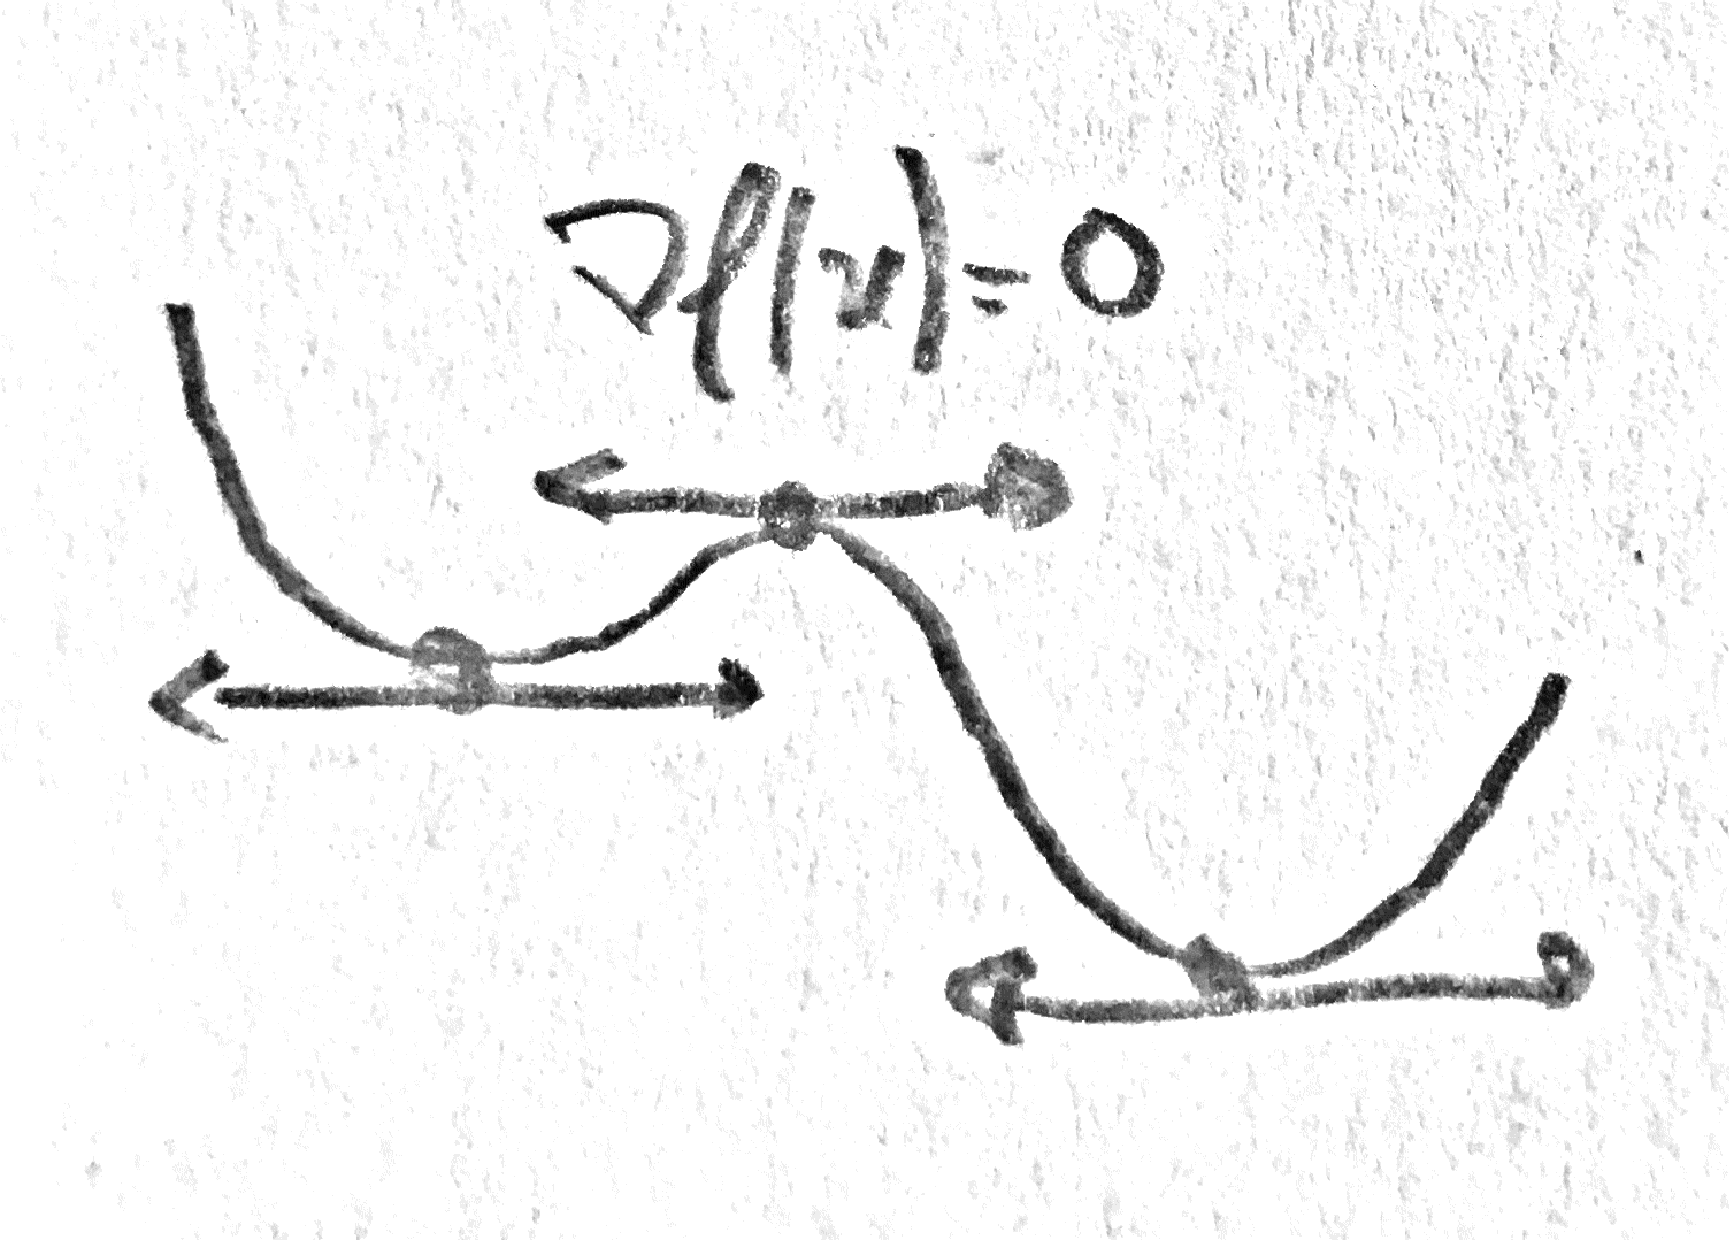
\includegraphics[width=.2\linewidth]{optim-smooth/first-order-1} \quad
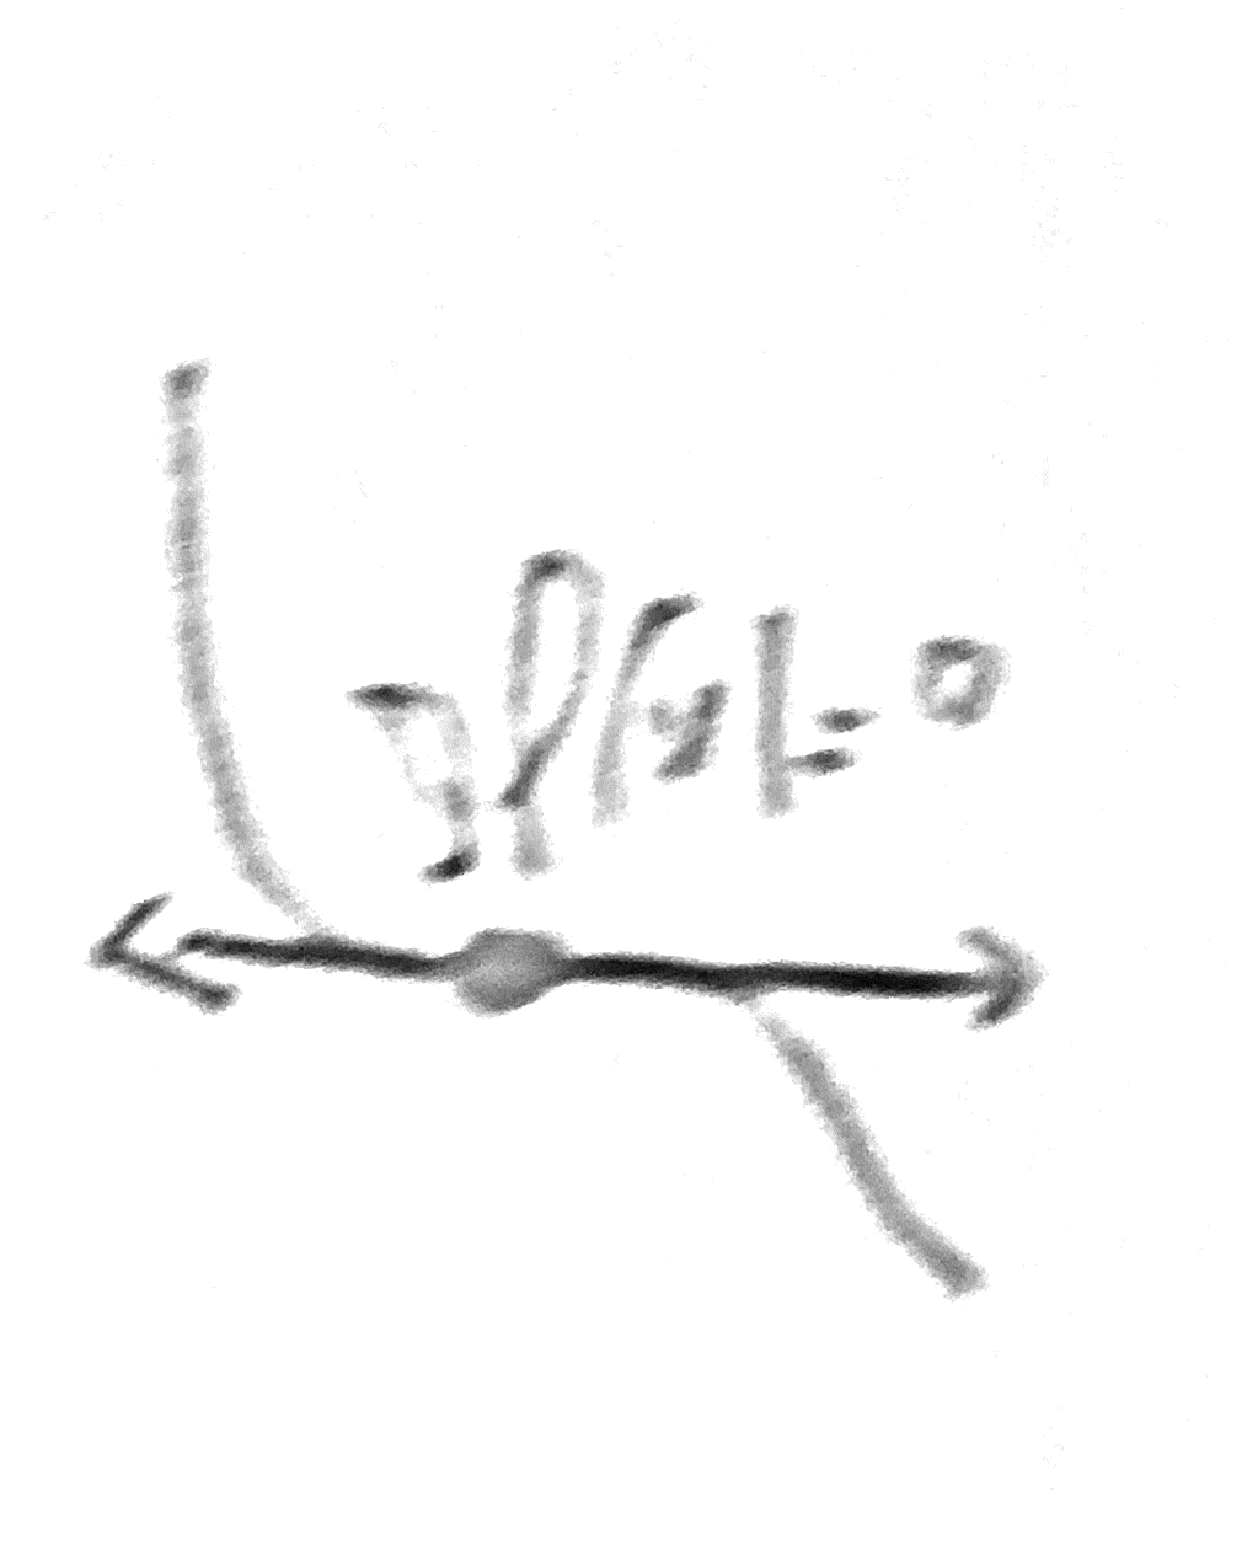
\includegraphics[width=.15\linewidth]{optim-smooth/first-order-2} \quad
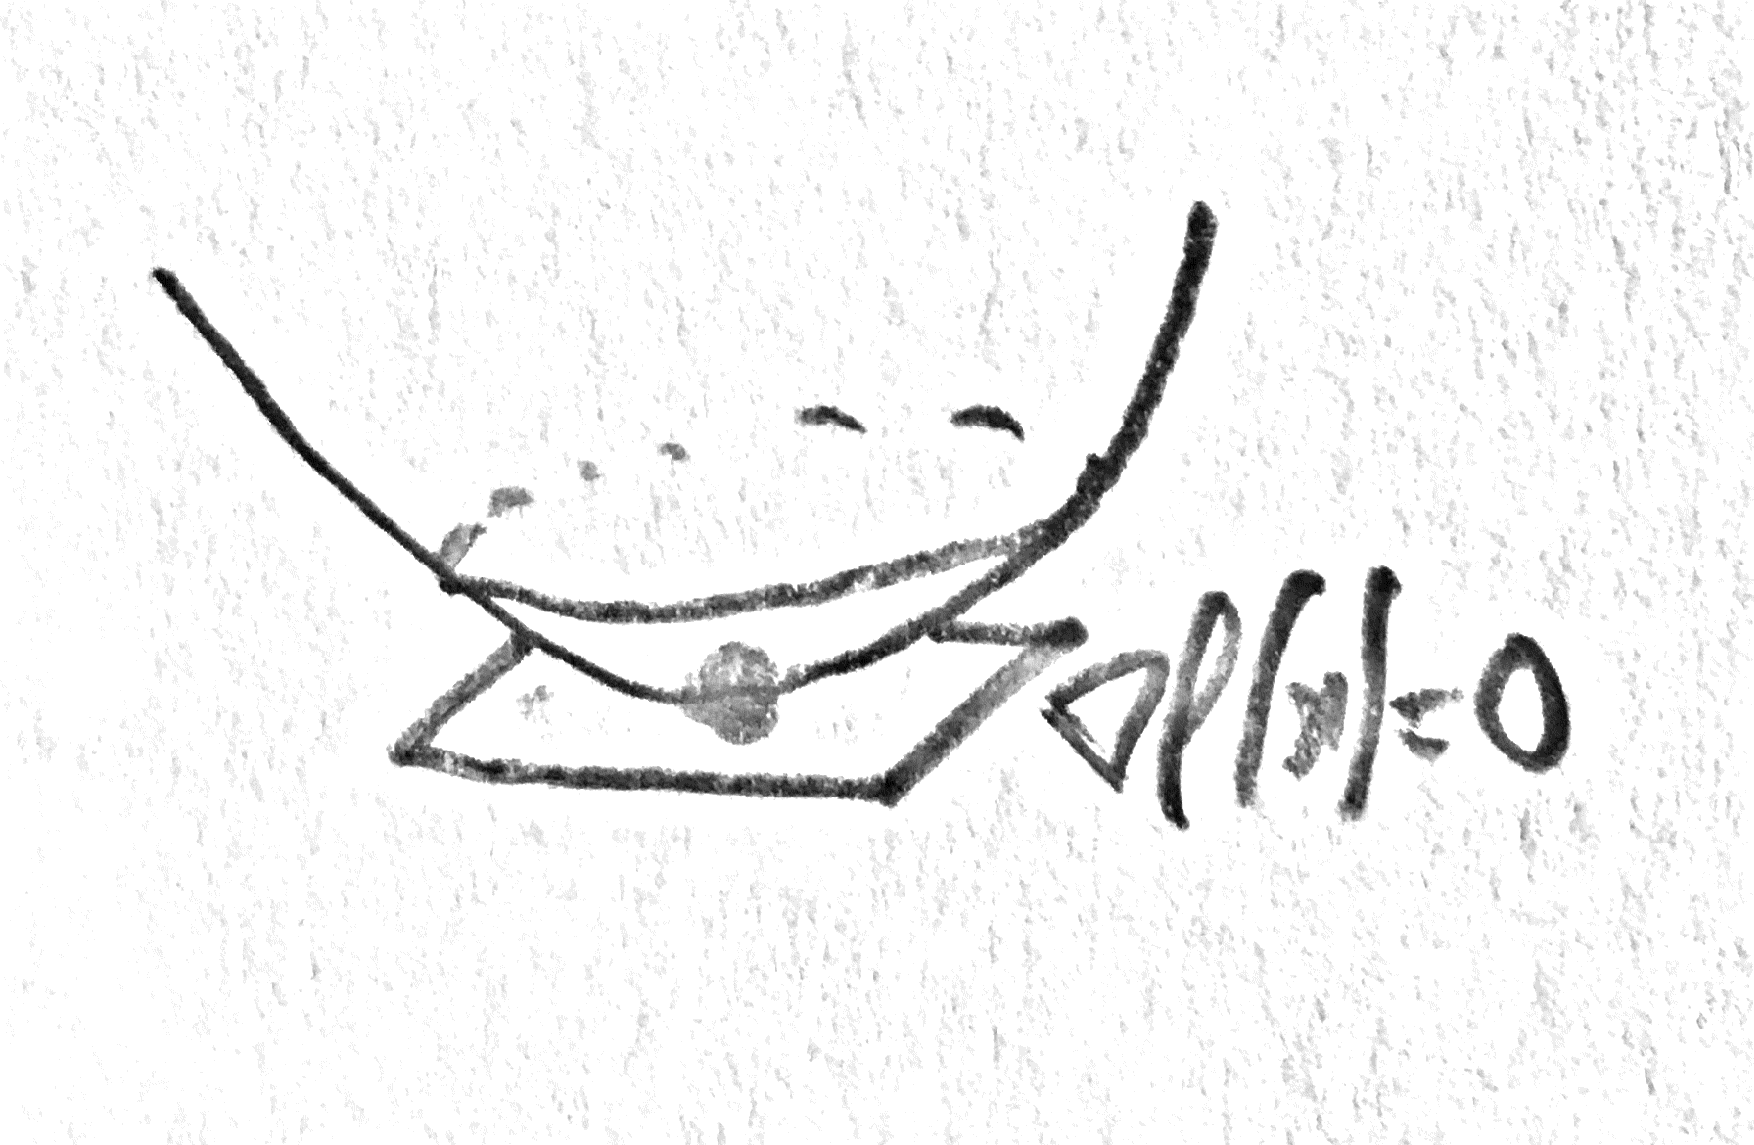
\includegraphics[width=.2\linewidth]{optim-smooth/first-order-3} 
\caption{\label{fig-first-order}
Function with local maxima/minima (left),  saddle point (middle) and global minimum (right). 
}
\end{figure}


\begin{prop} 
If $f$ is convex and $x^\star$ a local minimum, then $x^\star$ is also a global minimum.
If $f$ is differentiable and convex, 
\eq{
	x^\star \in \uargmin{x} f(x) 
	\quad\Longleftrightarrow\quad
	\nabla f(x^\star)=0.
}
\end{prop}
\begin{proof}
For any $x$, there exist $0<t<1$ small enough such that $tx + (1-t)x^\star$ is close enough to $x^\star$, and so since it is a local minimizer
\eq{
	f(x^\star) \leq f(tx + (1-t)x^\star) \leq t f(x) + (1-t) f(x^\star)
	\qarrq
	f(x^\star) \leq f(x)
}
and thus $x^\star$ is a global minimum.

For the second part, we already saw in~\eqref{prop-cs-min} the $\Leftarrow$ part. We assume that $\nabla f(x^\star)=0$. Since the graph of $x$ is above its tangent by convexity (as stated in Proposition~\ref{prop-above-tgt}), 
\eq{
	f(x) \geq f(x^\star) + \dotp{\nabla f(x^\star)}{x-x^\star} = f(x^\star).
}
\end{proof}

Thus in this case, optimizing a function is the same a solving an equation $\nabla f(x)=0$ (actually $p$ equations in $p$ unknown).
%
In most case it is impossible to solve this equation, but it often provides interesting information about solutions $x^\star$.



%%%%%%%%%%%%%%%%%%%%%%%%%%%%%%%%%%%%%%%%%%%%%%%%%%%%%%%%%%%%%%%%%%%%%%%%%%%%%%%%%%
\subsection{Least Squares}

The most important gradient formula is the one of the square loss~\eqref{eq-least-square}, which can be obtained by expanding the norm
\begin{align*}
	f(x+\epsilon) &= \frac{1}{2}\norm{Ax-y+A\epsilon}^2 = \frac{1}{2}\norm{Ax-y} + \dotp{Ax-y}{A\epsilon} + \frac{1}{2}\norm{A\epsilon}^2 \\
		&=f(x) + \dotp{\epsilon}{A^\top(Ax-y)} + o(\norm{\epsilon}).
\end{align*} 
Here, we have used the fact that $\norm{A\epsilon}^2 = o(\norm{\epsilon})$ and use the transpose matrix $A^\top$. 
%
This matrix is obtained by exchanging the rows and the columns, i.e. $A^\top = (A_{j,i})_{i=1,\ldots,n}^{j=1,\ldots,p}$, but the way it should be remember and used is that it obeys the following swapping rule of the inner product, 
\eq{
	\foralls (u,v) \in \RR^{p} \times \RR^n, \quad
	\dotp{A u}{v}_{\RR^n} = \dotp{u}{A^\top v}_{\RR^p}. 
}
Computing gradient for function involving linear operator will necessarily requires such a transposition step.
%
This computation shows that
\eql{\label{eq-grad-ls}
	\nabla f(x) = A^\top (A x - y). 
}
This implies that solutions $x^\star$ minimizing $f(x)$ satisfies the linear system $(A^\top A) x^\star = A^\top y$. 
%
If $A^\star A \in \RR^{p \times p}$ is invertible, then $f$ has a single minimizer, namely  
\eql{\label{eq-sol-leastsquare}
	x^\star = (A^\top A)^{-1} A^\top y.
}
This shows that in this case, $x^\star$ depends linearly on the data $y$, and the corresponding linear operator $(A^\top A)^{-1} A^\star$ is often called the Moore-Penrose pseudo-inverse of $A$ (which is not invertible in general, since typically $p \neq n$). 
%
The condition that $A^\top A$ is invertible is equivalent to $\ker(A)=\{0\}$, since 
\eq{
	A^\top A x = 0 \qarrq \norm{Ax}^2 = \dotp{A^\top A x}{x} = 0 \qarrq A x= 0.
}
In particular, if $n<p$ (under-determined regime, there is too much parameter or too few data) this can never holds. If $n \geq p$ and the features $x_i$ are ``random'' then $\ker(A)=\{0\}$ with probability one. In this overdetermined situation $n \geq p$,  $\ker(A)=\{0\}$ only holds if the features $\{a_i\}_{i=1}^n$ spans a linear space $\Im(A^\top)$ of dimension strictly smaller than the ambient dimension $p$.
 
%%%%%%%%%%%%%%%%%%%%%%%%%%%%%%%%%%%%%%%%%%%%%%%%%%%%%%%%%%%%%%%%%%%%%%%%%%%%%%%%%%
\subsection{Link with PCA}

Let us assume the $(a_i)_{i=1}^n$ are centered, i.e. $\sum_i a_i=0$. If this is not the case, one needs to replace
 $a_i$ by $a_i - m$ where $m \eqdef \frac{1}{n}\sum_{i=1}^n a_i \in \RR^p$ is the empirical mean. In this case, $\frac{C}{n} = A^\top A/n \in \RR^{p \times p}$ is the empirical covariance of the point cloud $(a_i)_i$, it encodes the covariances between the coordinates of the points. Denoting $a_i = (a_{i,1},\ldots,a_{i,p})^\top \in \RR^p$ (so that $A=(a_{i,j})_{i,j}$) the coordinates, one has
 \eq{
 	\foralls (k,\ell) \in \{1,\ldots,p\}^2, \quad
 	\frac{C_{k,\ell}}{n} = \frac{1}{n} \sum_{i=1}^n a_{i,k} a_{i,\ell}. 
 }
 In particular, $C_{k,k}/n$ is the variance along the axis $k$. More generally, for any unit vector $u \in \RR^p$, $\dotp{C u}{u}/n \geq 0$ is the variance along the axis $u$.
 
For instance, in dimension $p=2$, 
\eq{
	\frac{C}{n} = 
	\frac{1}{n}
	\begin{pmatrix}
		 \sum_{i=1}^n a_{i,1}^2 & \sum_{i=1}^n a_{i,1} a_{i,2} \\
		\sum_{i=1}^n a_{i,1}a_{i,2} & \sum_{i=1}^n a_{i,2}^2
	\end{pmatrix}.
}

Since $C$ is a symmetric, it diagonalizes in an ortho-basis $U=(u_1,\ldots,u_p) \in \RR^{p \times p}$. Here, the vectors $u_k \in \RR^p$ are stored in the columns of the matrix $U$. The diagonalization means that there exist scalars (the eigenvalues) $(\la_1,\ldots,\la_p)$ so that $(\frac{1}{n} C) u_k = \la_k u_k$. Since the matrix is orthogononal, $UU^\top = U^\top U = \Id_p$, and equivalently $U^{-1}=U^\top$. The diagonalization property can be conveniently written as $\frac{1}{n} C=U \diag(\la_k) U^\top$. One can thus re-write the covariance quadratic form in the basis $U$ as being a separable sum of $p$ squares
\eql{\label{eq-pca-decomp}
	\frac{1}{n}  \dotp{Cx}{x} = \dotp{U \diag(\la_k) U^\top x}{x}
	= \dotp{\diag(\la_k) (U^\top x)}{(U^\top x)}
	= \sum_{k=1}^p \la_k \dotp{x}{u_k}^2.
} 
Here $( U^\top x )_k = \dotp{x}{u_k}$ is the coordinate $k$ of $x$ in the basis $U$. Since $\dotp{Cx}{x}=\norm{Ax}^2$, this shows that all the eigenvalues $\la_k \geq 0$ are positive. 

\begin{figure}
\centering
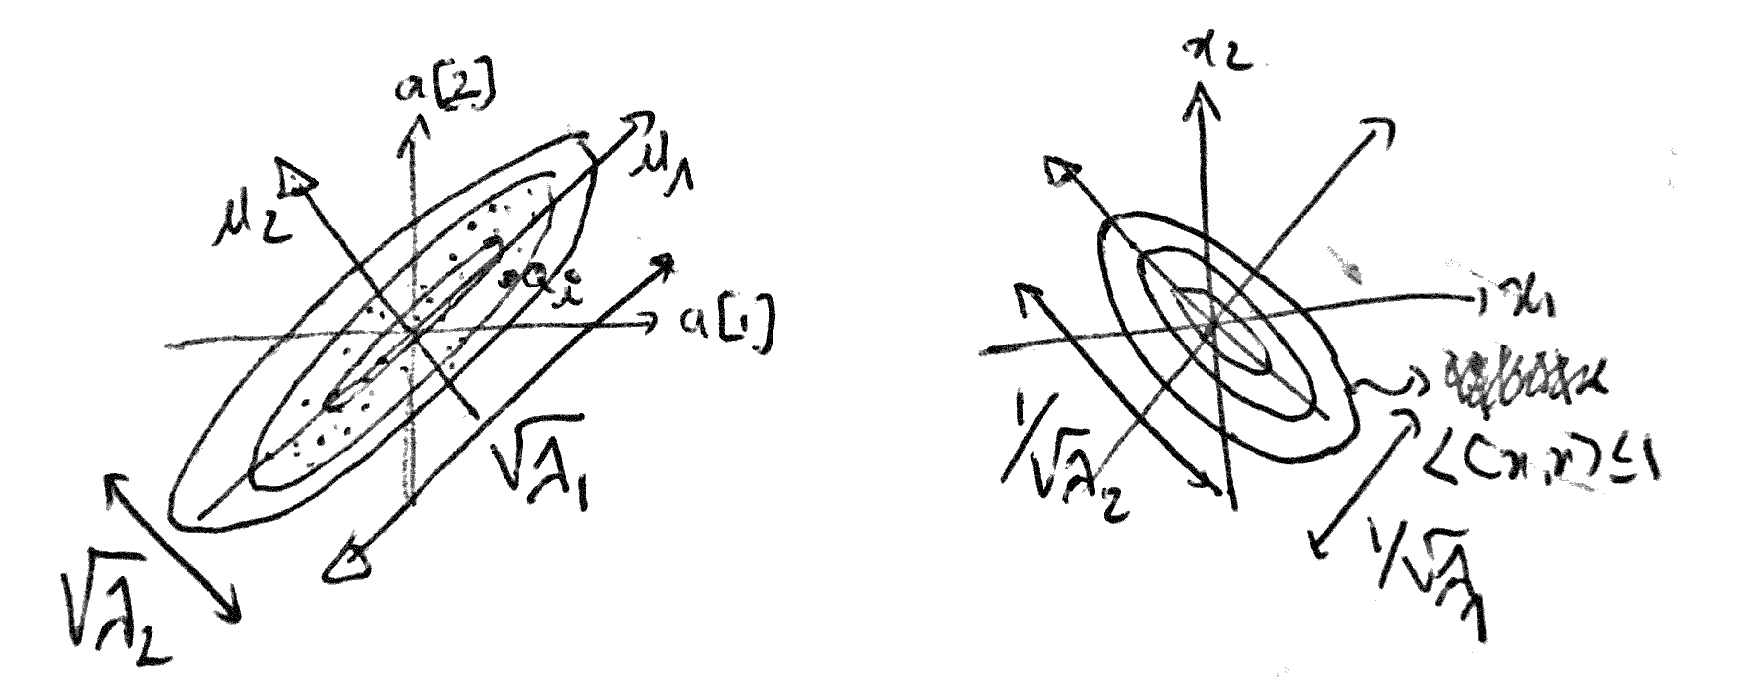
\includegraphics[width=.5\linewidth]{optim-smooth/link-pca}
\caption{\label{fig-link-pca}
Left: point clouds $(a_i)_i$ with associated PCA directions, right: quadratic part of $f(x)$.
}
\end{figure}

If one assumes that the eigenvalues are ordered $\la_1 \geq \la_2 \geq \ldots \geq \la_p$, then projecting the points $a_i$ on the first $m$ eigenvectors can be shown to be in some sense the best linear dimensionality reduction possible (see next paragraph), and it is called Principal Component Analysis (PCA). It is useful to perform compression or dimensionality reduction, but in practice, it is mostly used for data visualization in 2-D ($m=2$) and 3-D ($m=3$).

The matrix $C/n$ encodes the covariance, so one can approximate the point cloud by an ellipsoid whose main axes are the $(u_k)_k$ and the width along each axis is $\propto \sqrt{\la_k}$ (the standard deviations). 
%
If the data are approximately drawn from a Gaussian distribution, whose density is proportional to $\exp(\frac{-1}{2}\dotp{C^{-1}a}{a})$, then the fit is good.
%
This should be contrasted with the shape of quadratic part $\frac{1}{2}\dotp{Cx}{x}$ of $f(x)$, since the ellipsoid $\enscond{x}{\frac{1}{n}\dotp{Cx}{x} \leq 1}$ has the same main axes, but the widths are the inverse $1/\sqrt{\la_k}$. 
%
Figure~\ref{fig-link-pca} shows this in dimension $p=2$.



%%%%%%%%%%%%%%%%%%%%%%%%%%%%%%%%%%%%%%%%%%%%%%%%%%%%%%%%%%%%%%%%%%%%%%%%%%%%%%%%%%
\subsection{Classification}

We can do a similar computation for the gradient of the classification loss~\eqref{eq-classif}. Assuming that $L$ is differentiable, and using the Taylor expansion~\eqref{eq-grad-dfn} at point $-\diag(y) Ax$, one has 
\begin{align*}
	f(x+\epsilon) &= L( -\diag(y) Ax -\diag(y)  A\epsilon) \\
	&= L(-\diag(y) Ax) + \dotp{\nabla L( -\diag(y) Ax)}{ -\diag(y)  A\epsilon } + o(\norm{\diag(y)  A\epsilon}).
\end{align*} 
Using the fact that $o(\norm{\diag(y)  A\epsilon}) = o(\norm{\epsilon})$, one obtains
\begin{align*}
	f(x+\epsilon) &= f(x) + \dotp{\nabla L( -\diag(y) Ax)}{-\diag(y)  A\epsilon} + o(\norm{\epsilon}) \\
		 &=  f(x) + \dotp{-A^\top \diag(y) \nabla L( -\diag(y) Ax)}{\epsilon} + o(\norm{\epsilon}), 
\end{align*} 	
where we have used the fact that $(AB)^\top = B^\top A^\top$ and that $\diag(y)^\top=\diag(y)$. This shows that
\eq{
	\nabla f(x) = -A^\top \diag(y) \nabla L( -\diag(y) Ax). 
}
Since $L(z) = \sum_i \ell(z_i)$, one has $\nabla L(z) = (\ell'(z_i))_{i=1}^n$. For instance, for the logistic classification method, $\ell(u) = \log(1+\exp(u))$ so that $\ell'(u) = \frac{e^u}{1+e^u} \in [0,1]$ (which can be interpreted as a probability of predicting $+1$).


%%%%%%%%%%%%%%%%%%%%%%%%%%%%%%%%%%%%%%%%%%%%%%%%%%%%%%%%%%%%%%%%%%%%%%%%%%%%%%%%%%
\subsection{Chain Rule}

One can formalize the previous computation, if $f(x) = g(Bx)$ with $B \in \RR^{q \times p}$ and $g : \RR^q \rightarrow \RR$, then
\eq{
	f(x+\epsilon) = g(Bx + B\epsilon) = g(Bx) + \dotp{\nabla g(Bx)}{B \epsilon} + o(\norm{B \epsilon})
	= f(x) + \dotp{\epsilon}{B^\top \nabla g(Bx)} + o(\norm{\epsilon}), 
}
which shows that 
\eql{\label{eq-grad-composition-linear}
	\nabla ( g \circ B ) = B^\top \circ \nabla g \circ B
}
where ``$\circ$'' denotes the composition of functions.

To generalize this to composition of possibly non-linear functions, one needs to use the notion of differential. For a function $F : \RR^p \rightarrow \RR^q$, its differentiable at $x$ is a linear operator $\partial F(x) : \RR^{p} \rightarrow \RR^q$, i.e. it can be represented as a matrix (still denoted $\partial F(x)$) $\partial F(x) \in \RR^{q \times p}$.
%
The entries of this matrix are the partial differential, denoting $F(x)=(F_1(x), \ldots, F_q(x))$, 
\eq{
	\foralls (i,j) \in \{1,\ldots,q\} \times \{1,\ldots,p\}, \quad
	[ \partial F(x) ]_{i,j} \eqdef \frac{\partial F_i(x)}{\partial x_j}.
}
The function $F$ is then said to be differentiable at $x$ if and only if one has the following Taylor expansion 
\eql{\label{eq-differential-defn}
	F(x+\epsilon) = F(x) + [\partial F(x)](\epsilon) + o(\norm{\epsilon}).
}
where $[\partial F(x)](\epsilon)$ is the matrix-vector multiplication. As for the definition of the gradient, this matrix is the only one that satisfies this expansion, so it can be used as a way to compute this differential in practice.

For the special case $q=1$, i.e. if $f : \RR^p \rightarrow \RR$, then the differential $\partial f(x) \in \RR^{1 \times p}$ and the gradient $\nabla f(x) \in \RR^{p \times 1}$ are linked by equating the Taylor expansions~\eqref{eq-differential-defn} and~\eqref{eq-grad-dfn}
\eq{
	\foralls \epsilon \in \RR^p, \quad
	[\partial f(x)](\epsilon) = \dotp{\nabla f(x)}{\epsilon}	
	\quad\Leftrightarrow\quad
	[\partial f(x)](\epsilon) = \nabla f(x)^\top. 
}

The differential satisfies the following chain rule 
\eq{
	\partial( G \circ H)(x) = [\partial G(H(x))] \times [\partial H(x)] 
}
where ``$\times$'' is the matrix product. For instance, if $H : \RR^p \rightarrow \RR^q$ and $G = g : \RR^q \mapsto \RR$, then $f = g \circ H : \RR^p \rightarrow \RR$ and one can compute its gradient as follow
\eq{
	\nabla f(x) = (\partial f(x))^\top = \pa{ [\partial g(H(x))] \times [\partial H(x)] }^\top
	= [\partial H(x)]^\top \times [\partial g(H(x))]^\top
	= [\partial H(x)]^\top \times \nabla g(H(x)).
}
When $H(x)=Bx$ is linear, one recovers formula~\eqref{eq-grad-composition-linear}.


%%%%%%%%%%%%%%%%%%%%%%%%%%%%%%%%%%%%%%%%%%%%%%%%%%%%%%%%%%%%%%%%%%%%%%%%%%%%%%%%%%
%%%%%%%%%%%%%%%%%%%%%%%%%%%%%%%%%%%%%%%%%%%%%%%%%%%%%%%%%%%%%%%%%%%%%%%%%%%%%%%%%%
%%%%%%%%%%%%%%%%%%%%%%%%%%%%%%%%%%%%%%%%%%%%%%%%%%%%%%%%%%%%%%%%%%%%%%%%%%%%%%%%%%
\section{Gradient Descent Algorithm}
\label{sec-grad-desc-basic}


%%%%%%%%%%%%%%%%%%%%%%%%%%%%%%%%%%%%%%%%%%%%%%%%%%%%%%%%%%%%%%%%%%%%%%%%%%%%%%%%%%
\subsection{Steepest Descent Direction}

The Taylor expansion~\eqref{eq-grad-dfn} computes an affine approximation of the function $f$ near $x$, since it can be written as
\eq{
	f(z) = T_x(z) + o(\norm{x-z})
	\qwhereq
	T_x(z) \eqdef f(x) + \dotp{\nabla f(x)}{z-x}, 
}
see Fig.~\ref{fig-expansion-taylor}. First order methods operate by locally replacing $f$ by $T_x$.


\begin{figure}
\centering
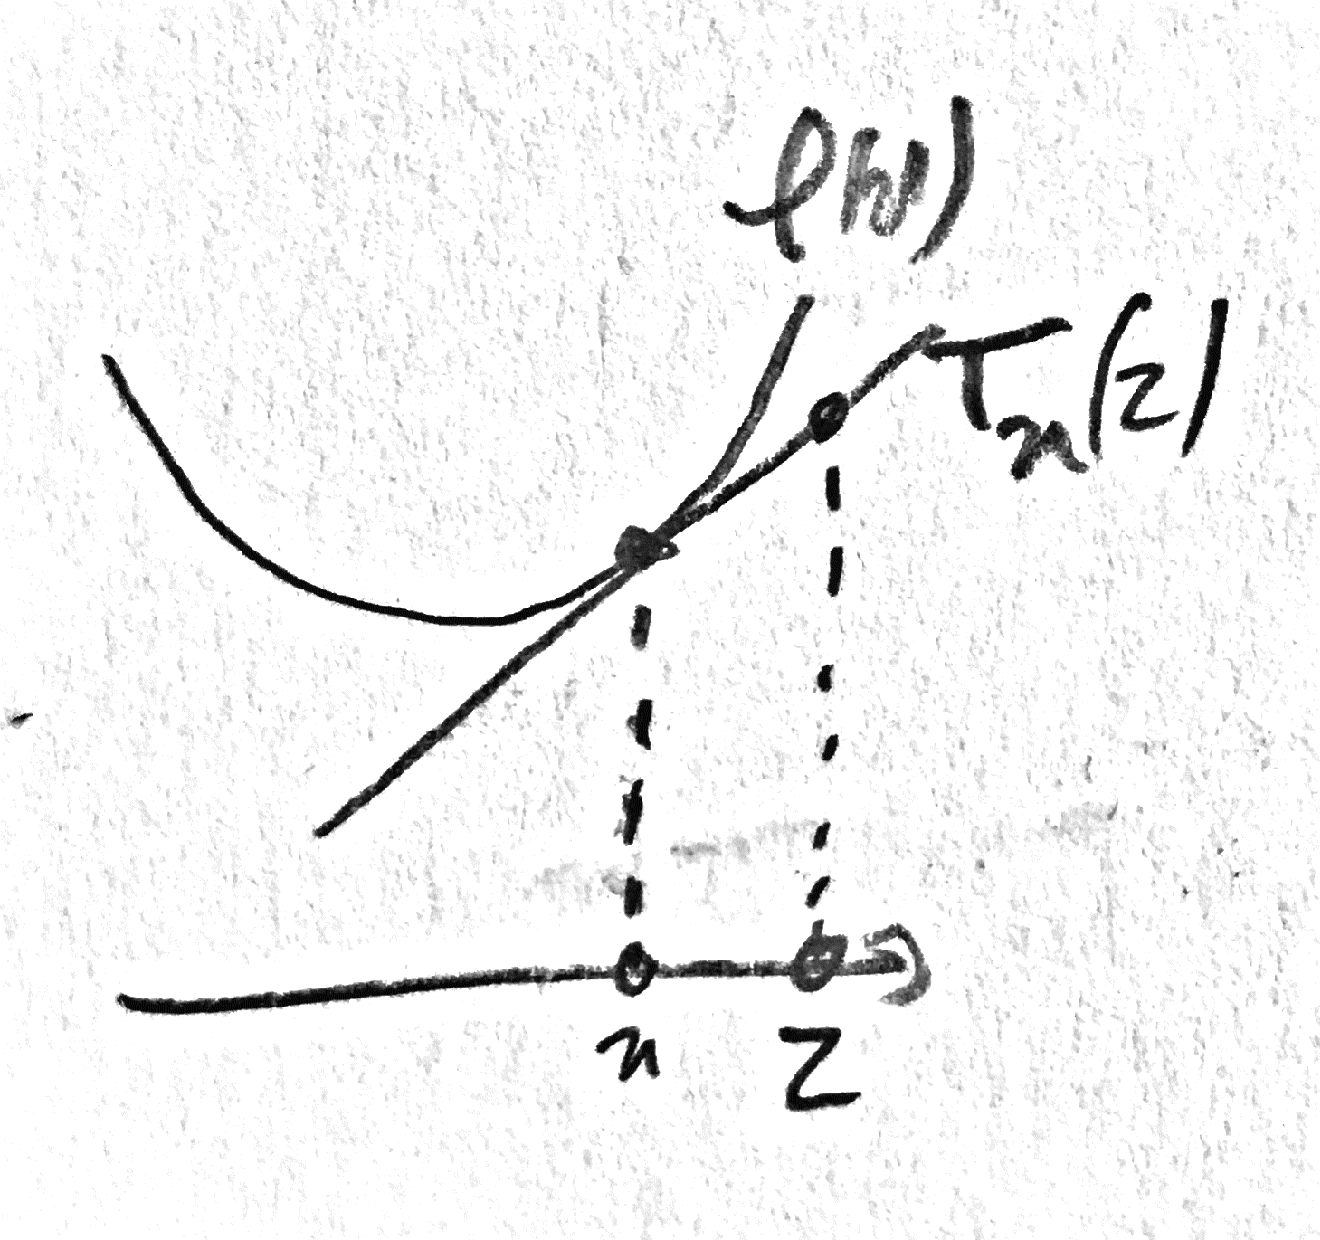
\includegraphics[width=.2\linewidth]{optim-smooth/taylor-exp-1} \quad
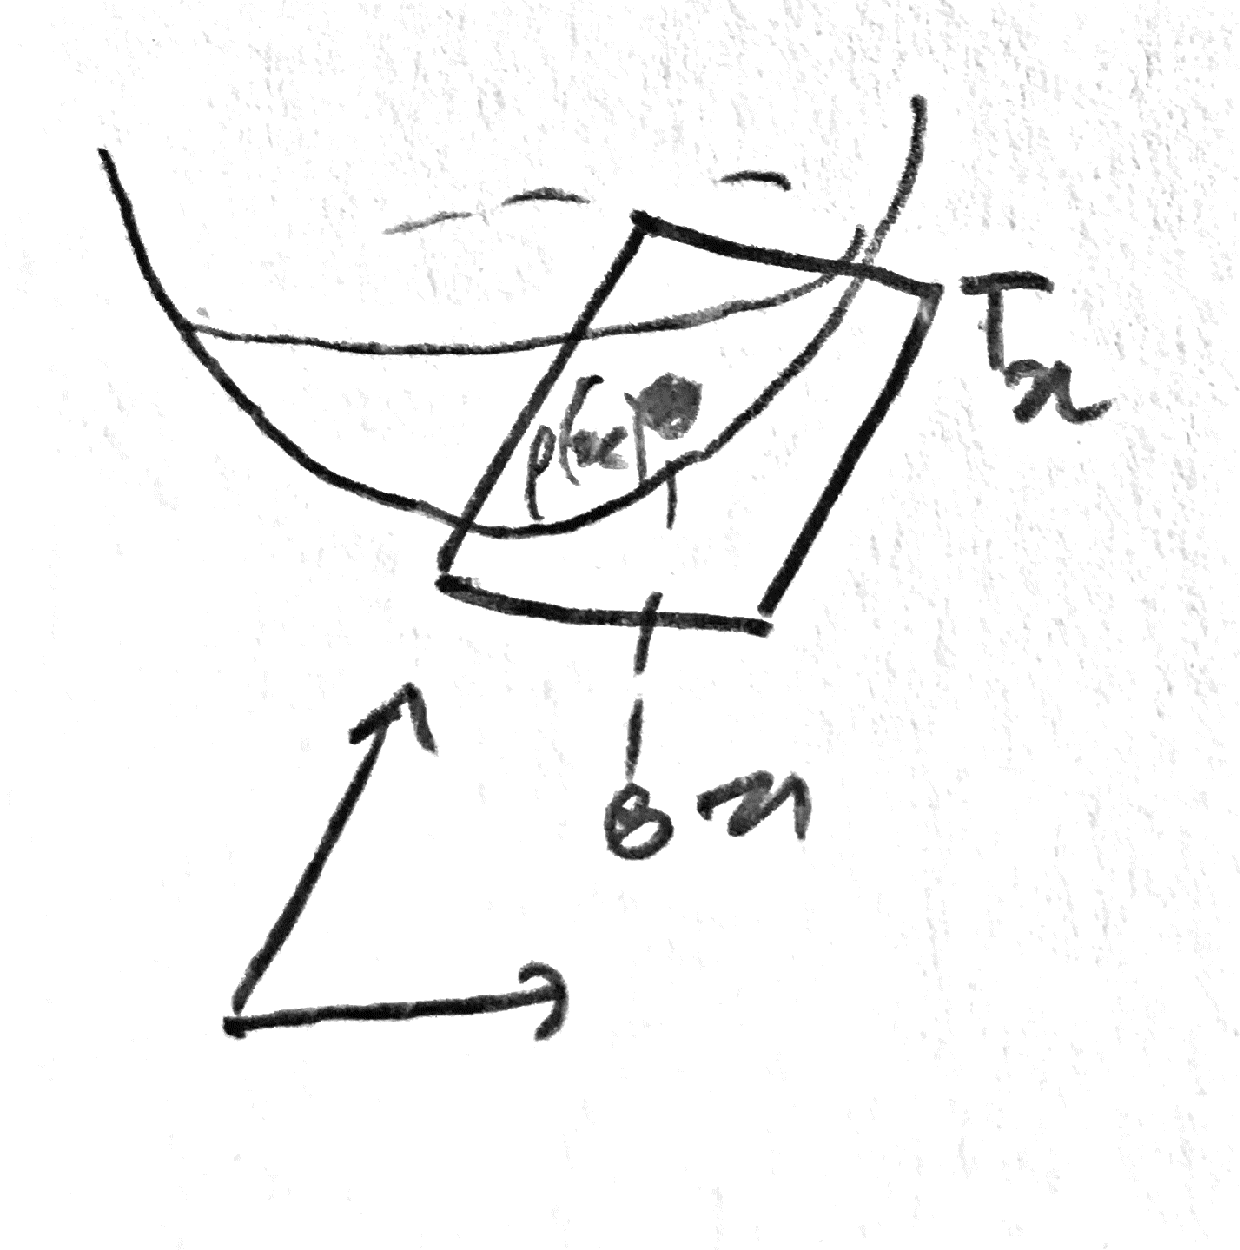
\includegraphics[width=.18\linewidth]{optim-smooth/taylor-exp-2} \quad
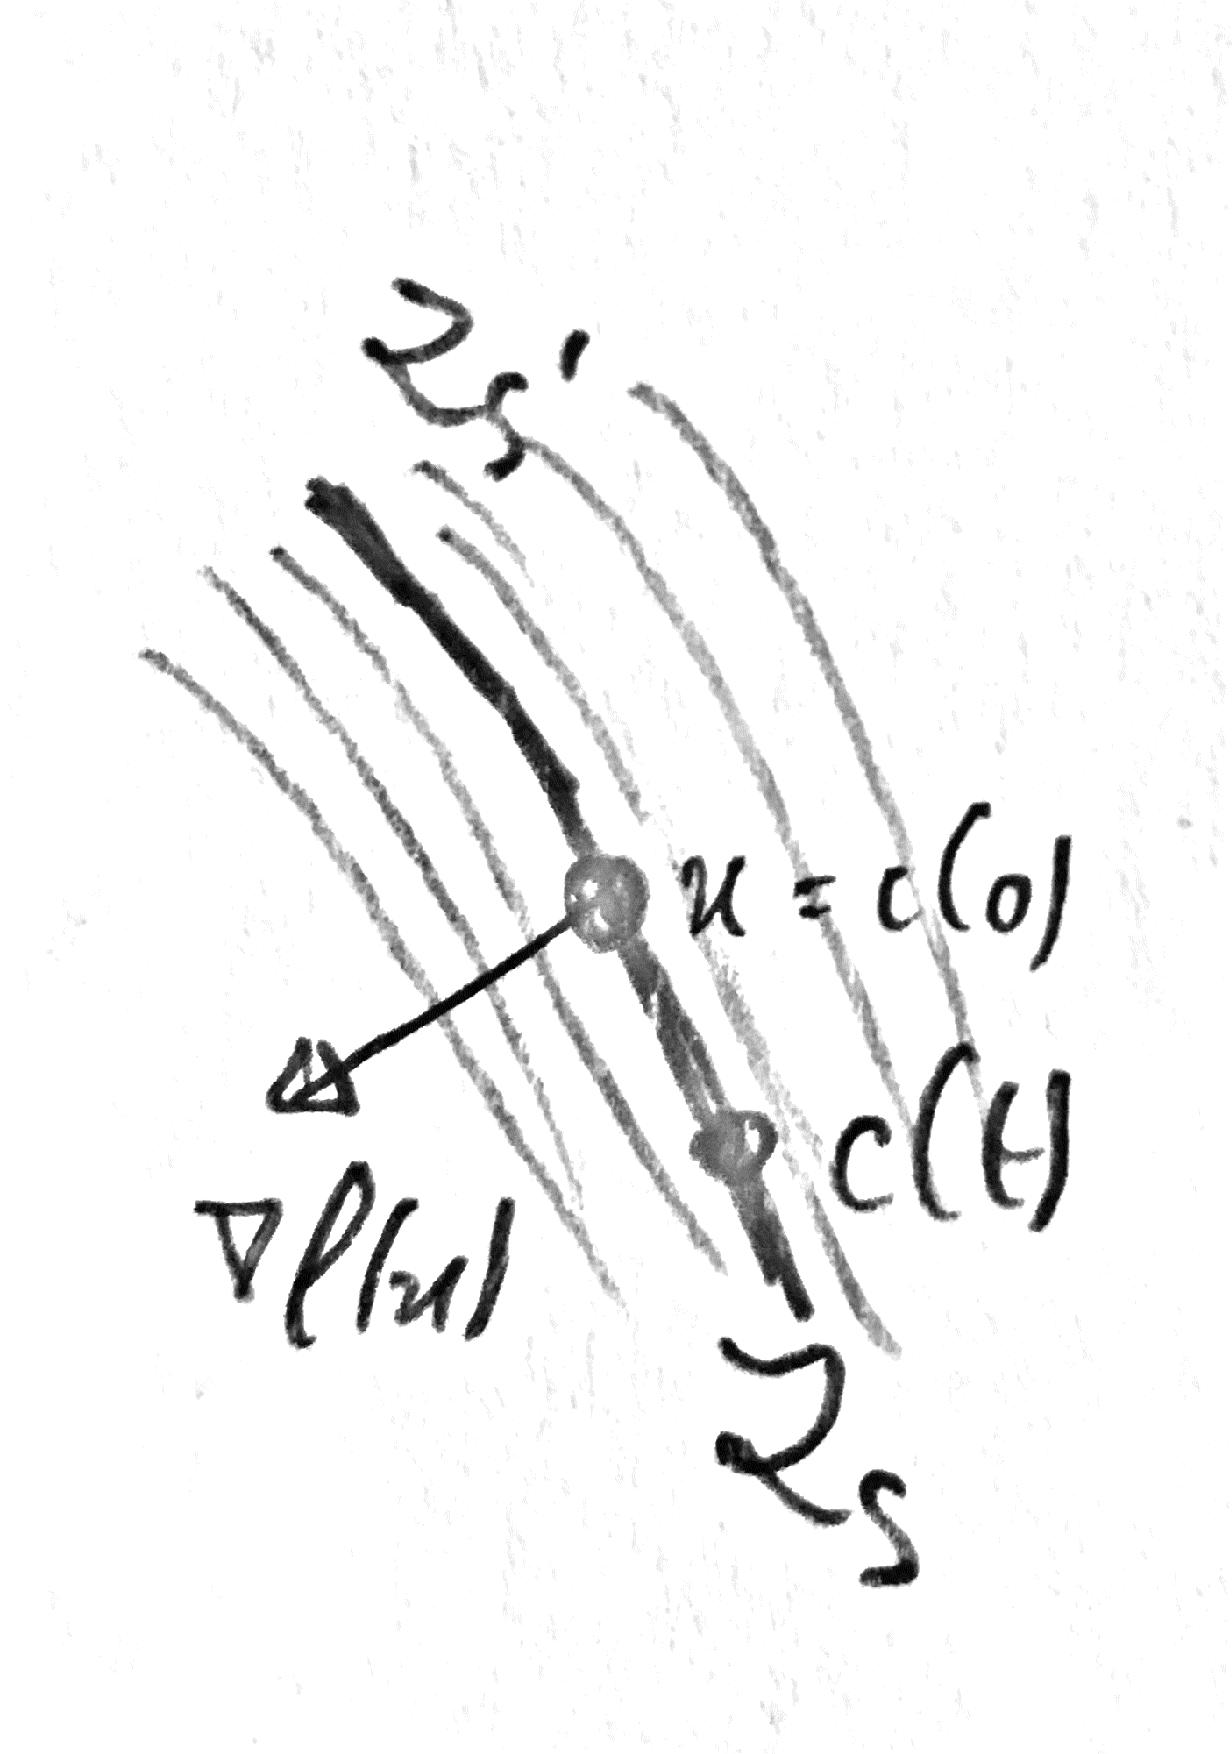
\includegraphics[width=.18\linewidth]{optim-smooth/level-sets-1} \quad
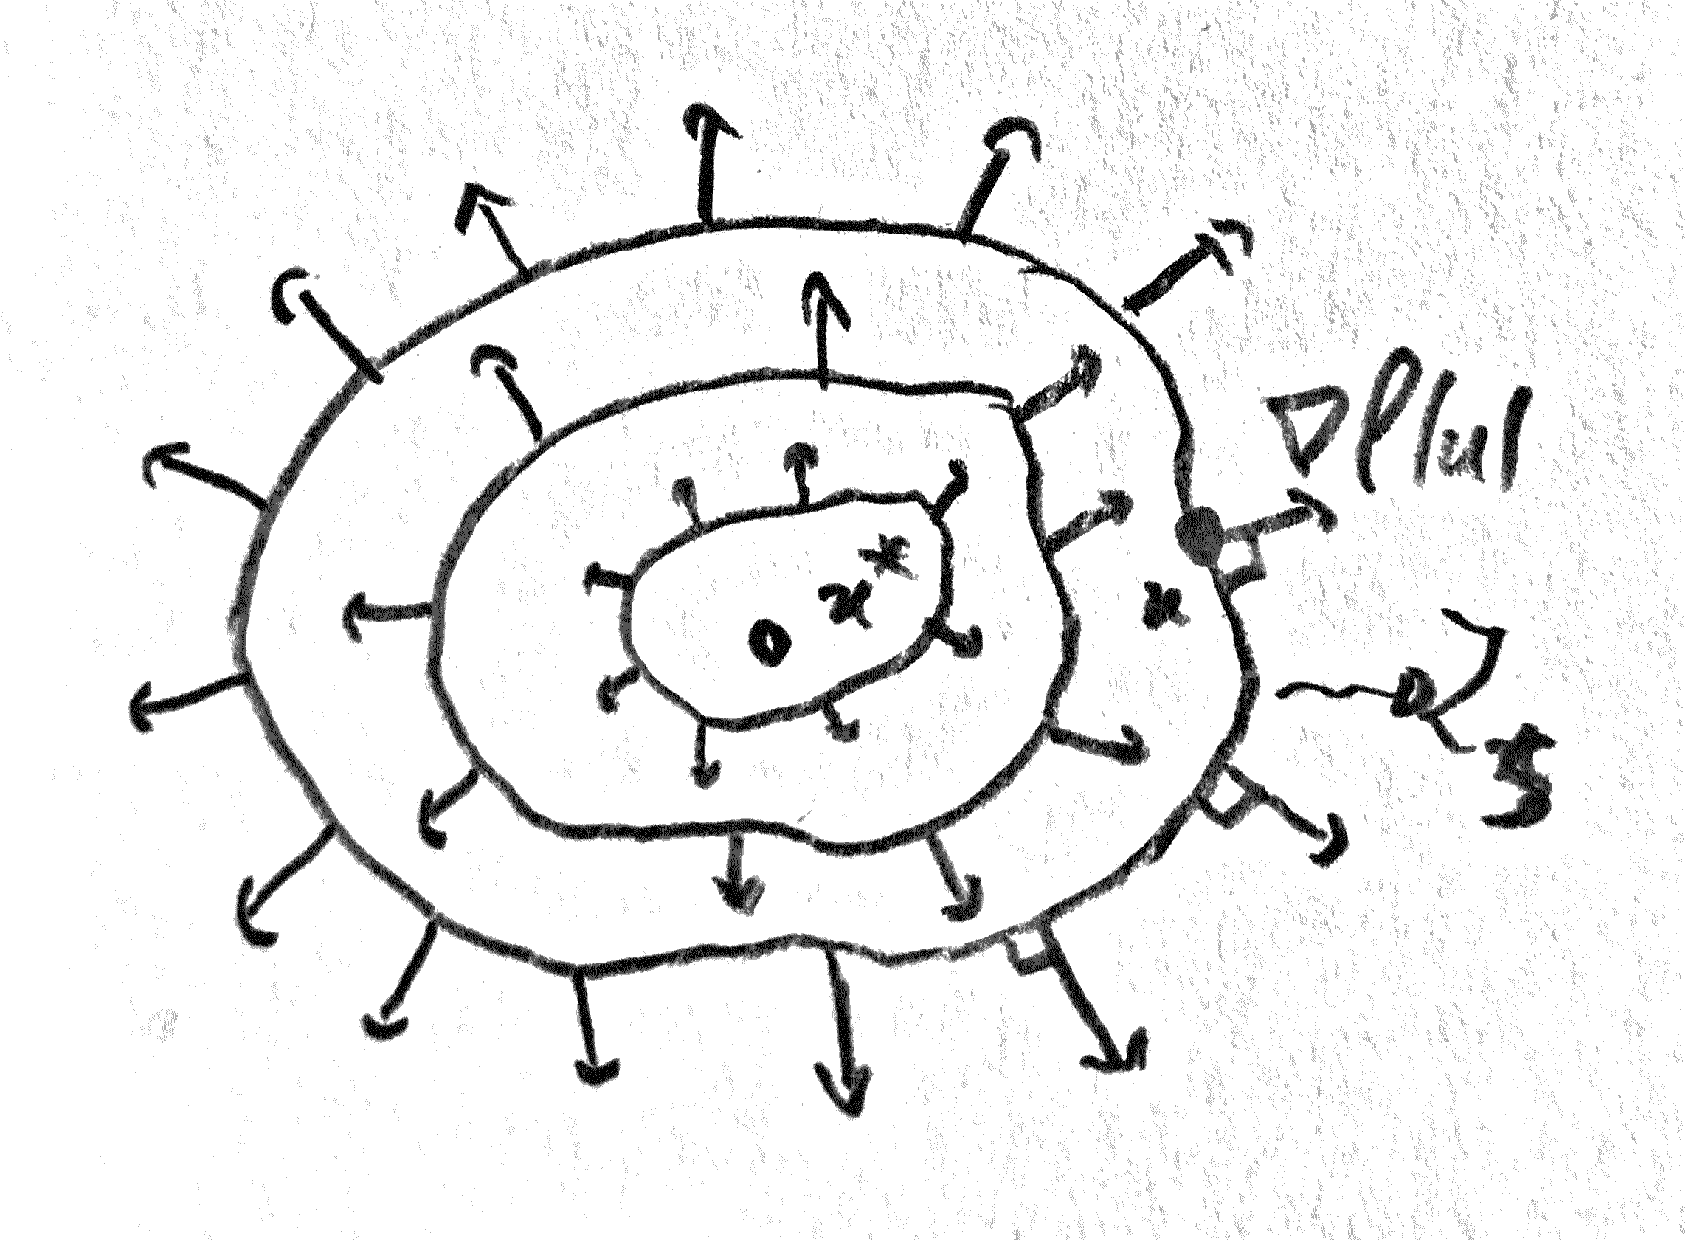
\includegraphics[width=.25\linewidth]{optim-smooth/level-sets-2} 
\caption{\label{fig-expansion-taylor}
	Left: First order Taylor expansion in 1-D and 2-D.
	Right: orthogonality of gradient and level sets and schematic of the proof.
}
\end{figure}

The gradient $\nabla f(x)$ should be understood as a direction along which the function increases. This means that to improve the value of the function, one should move in the direction $-\nabla f(x)$. Given some fixed $x$, let us look as the function $f$ along the 1-D half line 
\eq{ 
	\tau \in \RR^+ = [0,+\infty[ \longmapsto f(x-\tau \nabla f(x)) \in \RR.
}
If $f$ is differentiable at $x$, one has 
\eq{
	f(x-\tau \nabla f(x)) = f(x) - \tau \dotp{\nabla f(x)}{\nabla f(x)} + o(\tau)
		= f(x) - \tau \norm{\nabla f(x)}^2 + o(\tau).
}
So there are two possibility: either $\nabla f(x)=0$, in which case we are already at a minimum (possibly a local minimizer if the function is non-convex) or if $\tau$ is chosen small enough, 
\eq{
	f(x-\tau \nabla f(x)) < f(x)
} 
which means that moving from $x$ to $x-\tau \nabla f(x)$ has improved the objective function. 

\begin{rem}[Orthogonality to level sets]
	The level sets of $f$ are the sets of point sharing the same value of $f$, i.e. for any $s \in \RR$
	\eq{
		\Ll_s \eqdef \enscond{x}{f(x)=s}.		
	}
	At some $x \in \RR^p$, denoting $s=f(x)$, then $x \in \Ll_s$ ($x$ belong to its level set). The gradient vector $\nabla f(x)$ is orthogonal to the level set (as shown on Fig.~\ref{fig-expansion-taylor} right), and points toward level set of higher value (which is consistent with the previous computation showing that it is a valid ascent direction). 
	%
	Indeed, lets consider around $x$ inside $\Ll_s$ a smooth curve of the form $t \in \RR \mapsto c(t)$ where $c(0)=x$. 
	%	
	Then the function $h(t) \eqdef f(c(t))$ is constant $h(t)=s$  since $c(t)$ belong to the level set. So $h'(t)=0$. But at the same time, we can compute its derivate at $t=0$ as follow
	\eq{
		h(t) = f(c(0) + t c'(0) + o(t)) = h(0) + \de \dotp{c'(0)}{\nabla f(c(0))} + o(t)
	}	
	i.e. $h'(0) = \dotp{c'(0)}{\nabla f(x)}=0$, so that $\nabla f(x)$ is orthogonal to the tangent $c'(0)$ of the curve $c$, which lies in the tangent plane of $\Ll_s$  (as shown on Fig.~\ref{fig-expansion-taylor}, right).  Since the curve $c$ is arbitrary, the whole tangent plane is thus orthogonal to $\nabla f(x)$. 
\end{rem}

\begin{rem}[Local optimal descent direction]
	One can prove something even stronger, that among all possible direction $u$ with $\norm{u}=r$, $r \frac{\nabla f(x)}{\norm{\nabla f(x)}}$ becomes the optimal one as $r \rightarrow 0$ (so for very small step this is locally the best choice), more precisely, 
\eq{
	\frac{1}{r} \uargmin{\norm{u}=r} f(x + u) \overset{r \rightarrow 0}{\longrightarrow} -\frac{\nabla f(x)}{\norm{\nabla f(x)}}.
}
Indeed, introducing a Lagrange multiplier $\la \in \RR$ for this constraint optimization problem, one obtains that the optimal $u$ satisfies $\nabla f(x+u) = \la u$ and $\norm{u}=r$. Thus $\frac{u}{r} =\pm \frac{\nabla f(x+u)}{\norm{\nabla f(x+u)}}$, and assuming that $\nabla f$ is continuous, when $\norm{u}=r \rightarrow 0$, this converges to $\frac{u}{\norm{u}} = \pm\frac{\nabla f(x)}{\norm{\nabla f(x)}}$. The sign $\pm$ should be $+1$ to obtain a maximizer and $-1$ for the minimizer.
\end{rem}


%%%%%%%%%%%%%%%%%%%%%%%%%%%%%%%%%%%%%%%%%%%%%%%%%%%%%%%%%%%%%%%%%%%%%%%%%%%%%%%%%%
\subsection{Gradient Descent}

The gradient descent algorithm reads, starting with some $x_0 \in \RR^p$
\eql{\label{eq-grad-desc}
	x_{k+1} \eqdef x_k - \tau_k \nabla f(x_k)
}
where $\tau_k>0$ is the step size (also called learning rate). For a small enough $\tau_k$, the previous discussion shows that the function $f$ is decaying through the iteration. So intuitively, to ensure convergence, $\tau_k$ should be chosen small enough, but not too small so that the algorithm is as fast as possible.
%
In general, one use a fix step size $\tau_k=\tau$, or try to adapt $\tau_k$ at each iteration (see Fig.~\ref{fig-gradesc}). 


\begin{figure}
\centering
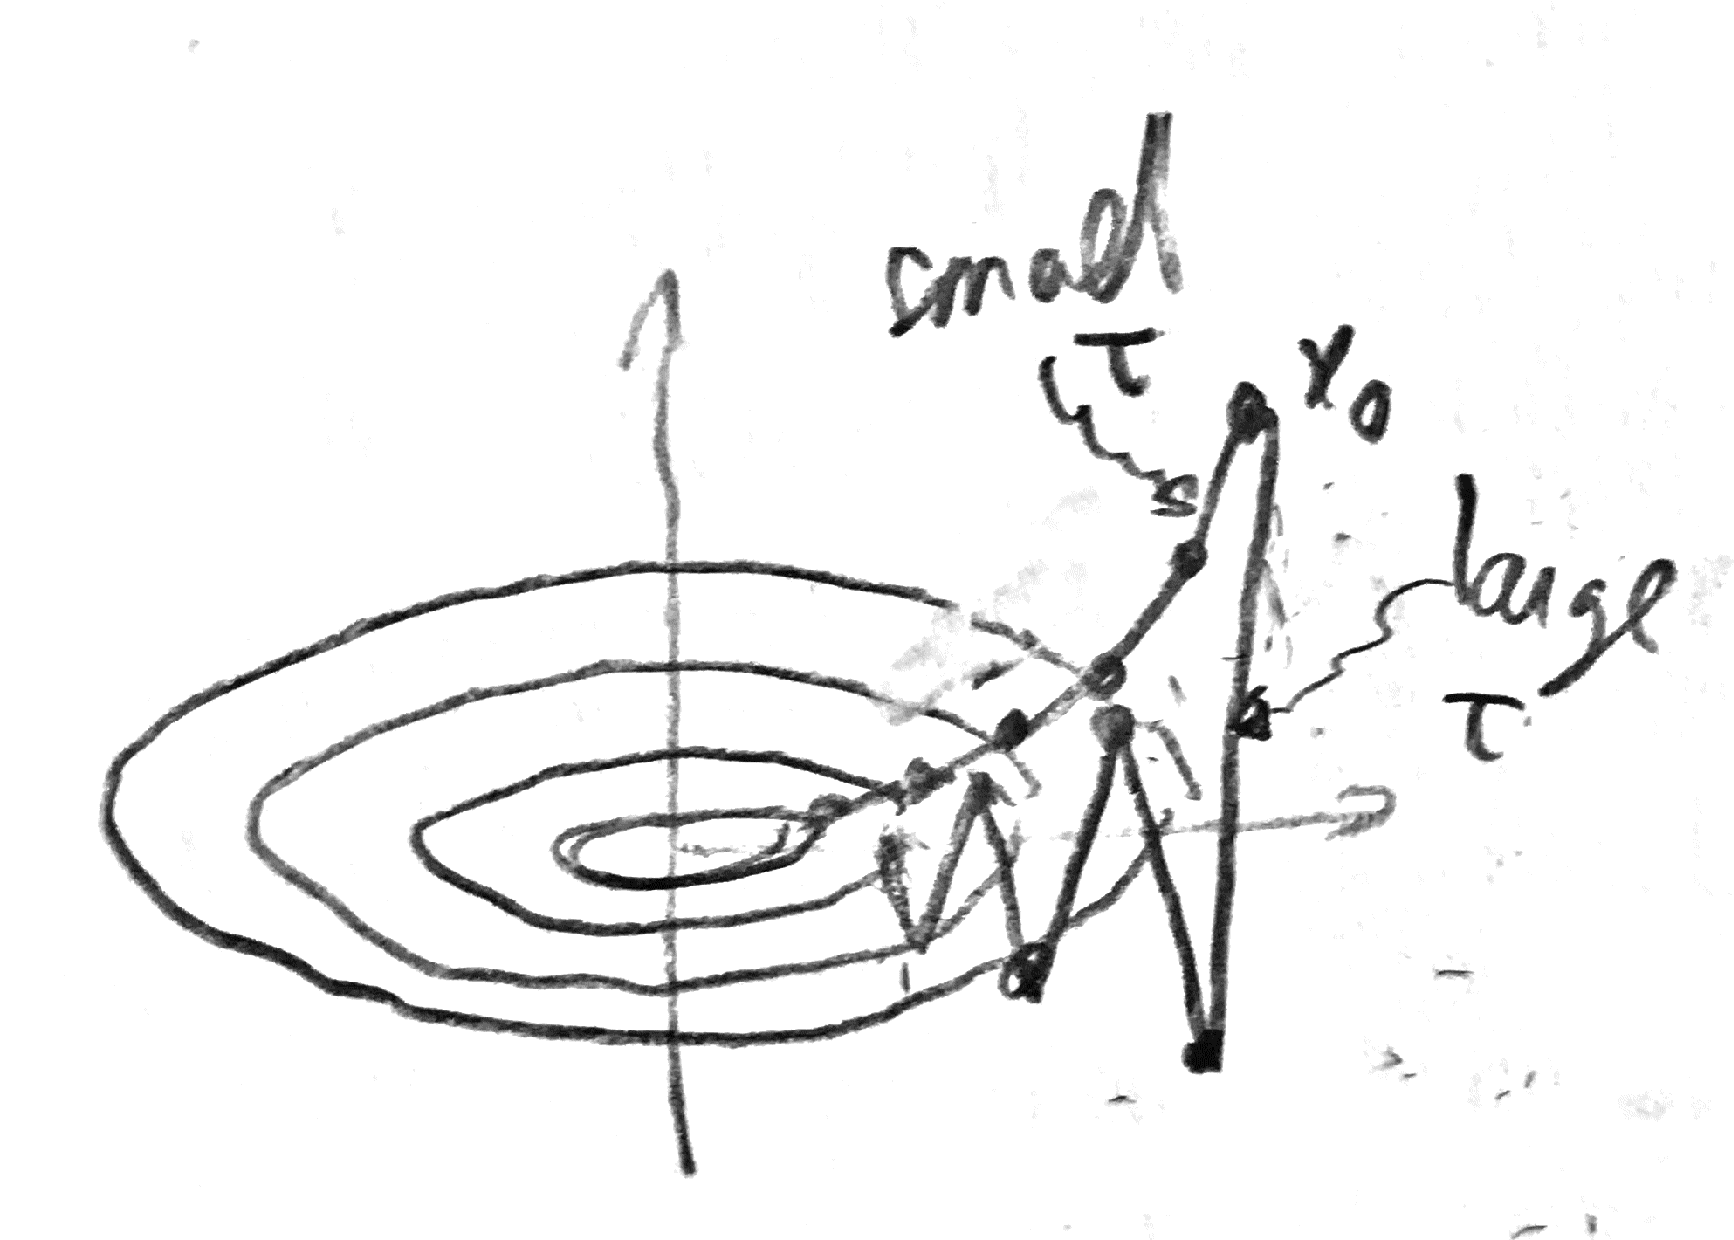
\includegraphics[width=.3\linewidth]{optim-smooth/grad-desc-1} \quad
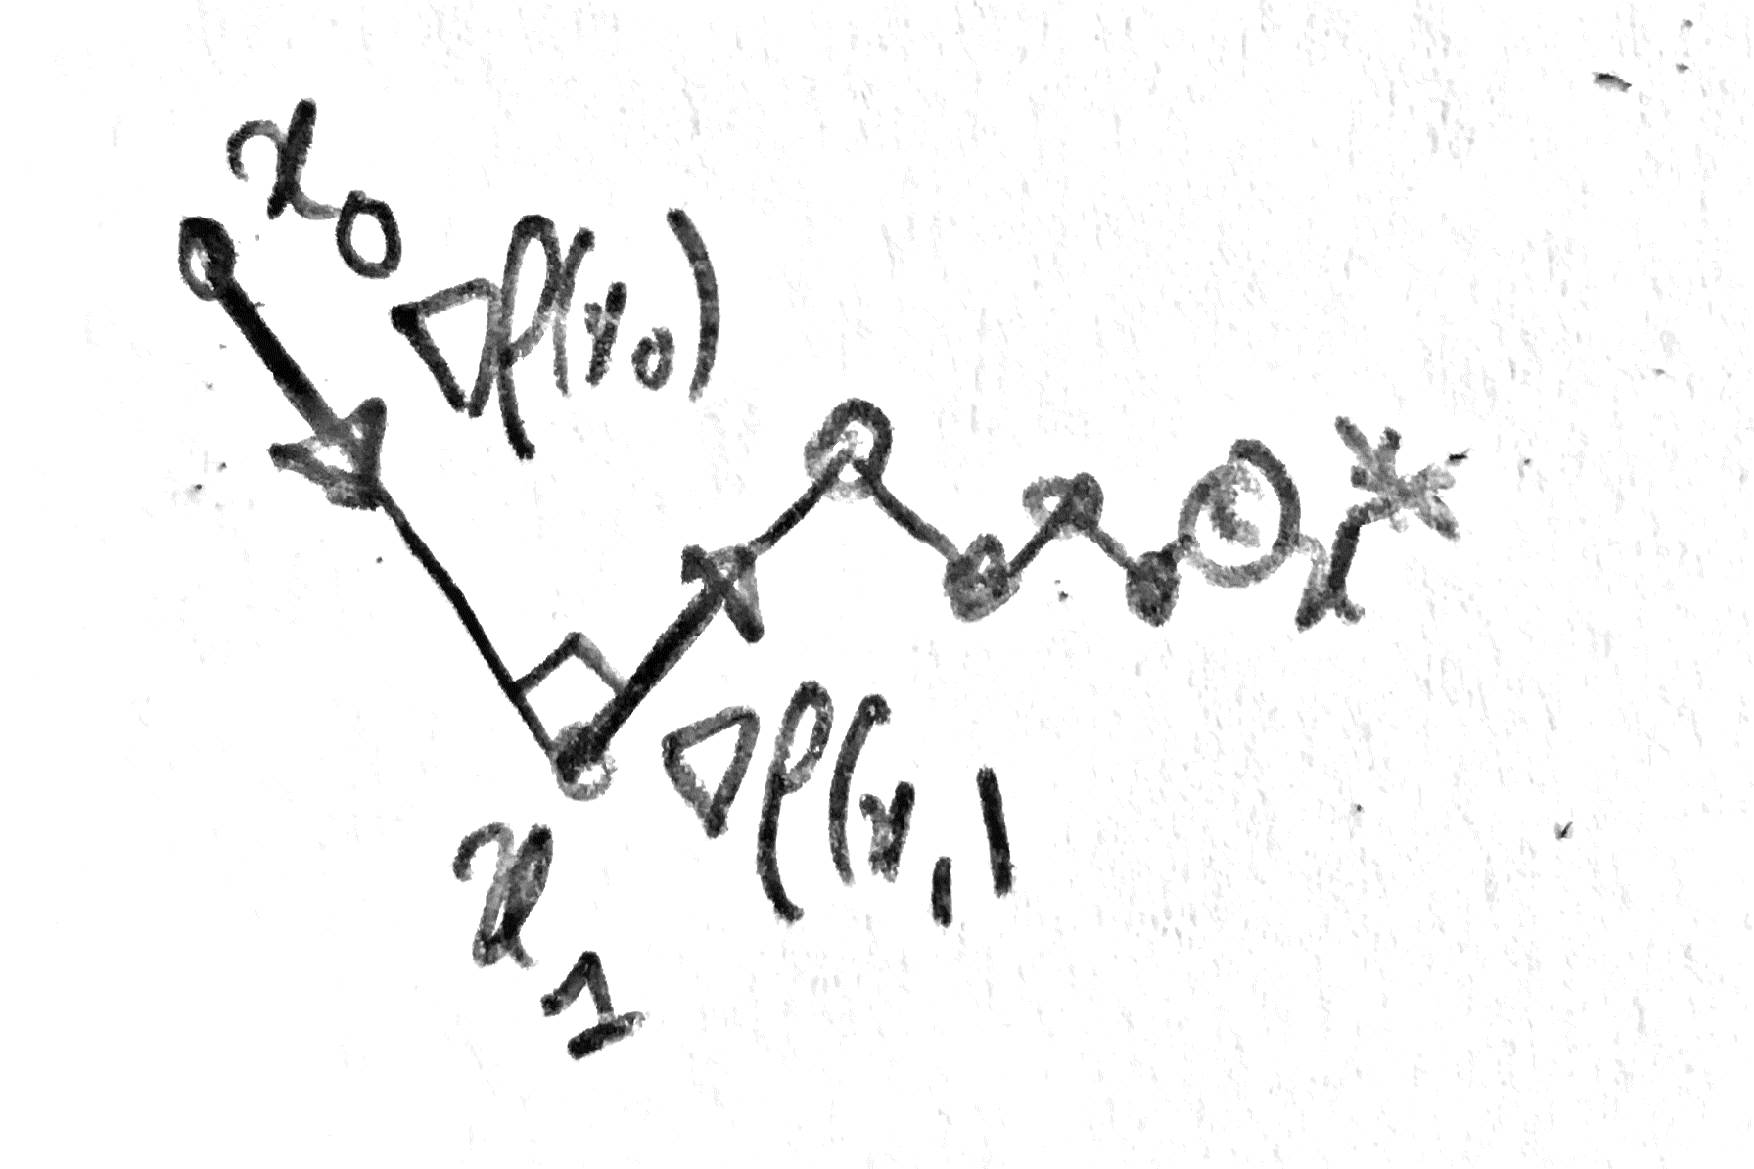
\includegraphics[width=.3\linewidth]{optim-smooth/grad-desc-2} 
\caption{\label{fig-gradesc}
Influence of $\tau$ on the gradient descent (left) and optimal step size choice (right).
}
\end{figure}


\begin{rem}[Greedy choice]
Although this is in general too costly to perform exactly, one can use a ``greedy'' choice, where the step size is optimal at each iteration, i.e. 
\eq{
	\tau_k \eqdef \uargmin{\tau} h(\tau) \eqdef f(x_k-\tau \nabla f(x_k)).
}
Here $h(\tau)$ is a function of a single variable. One can compute the derivative of $h$ as
\eq{
	h(\tau+\de) = f(x_k-\tau \nabla f(x_k) - \de \nabla f(x_k)) = f(x_k-\tau \nabla f(x_k))- \dotp{\nabla f(x_k-\tau \nabla f(x_k))}{ \nabla f(x_k)} + o(\de).
}
One note that at $\tau=\tau_k$, $\nabla f(x_k-\tau \nabla f(x_k))=\nabla f(x_{k+1})$ by definition of $x_{k+1}$ in~\eqref{eq-grad-desc}. 
%
Such an optimal $\tau=\tau_k$ is thus characterized by
\eq{
	h'(\tau_k) = - \dotp{\nabla f(x_k)}{\nabla f(x_{k+1})} = 0.
}
This means that for this greedy algorithm, two successive descent direction $\nabla f(x_k)$ and $\nabla f(x_{k+1})$ are orthogonal (see Fig.~\ref{fig-gradesc}).
\end{rem}

\begin{rem}[Armijo rule]
	Instead of looking for the optimal $\tau$, one can looks for an admissible $\tau$ which guarantees a large enough decay of the functional, in order to ensure convergence of the descent. 
	%
	Given some parameter $0<\al<1$ (which should be actually smaller than $1/2$ in order to ensure a sufficient decay), one consider a $\tau$ to be valid for a descent direction $d_k$ (for instance $d_k=-\nabla f(x_k)$) if it satisfies
	\eql{\label{eq-armijo-rule}
		f(x_k+\tau d_k) \leq f(x_k) + \al \tau \dotp{d_k}{\nabla f(x_k)}
	} 
	For small $\tau$, one has $f(x_k+\tau d_k) = f(x_k) + \tau \dotp{d_k}{\nabla f(x_k)}$, so that, assuming $d_k$ is a valid descent direction (i.e $\dotp{d_k}{\nabla f(x_k)}<0$),  condition~\eqref{eq-armijo-rule} will always be satisfied for $\tau$ small enough (if $f$ is convex, the set of allowable $\tau$ is of the form $[0,\tau_{\max}]$). 
	%
	In practice, one perform gradient descent by initializing $\tau$ very large, and decaying it $\tau \leftarrow \be \tau$ (for $\be < 1$) until~\eqref{eq-armijo-rule} is satisfied. 
	%
	This approach is often called ``backtracking'' line search. 
\end{rem}



%%%%%%%%%%%%%%%%%%%%%%%%%%%%%%%%%%%%%%%%%%%%%%%%%%%%%%%%%%%%%%%%%%%%%%%%%%%%%%%%%%
%%%%%%%%%%%%%%%%%%%%%%%%%%%%%%%%%%%%%%%%%%%%%%%%%%%%%%%%%%%%%%%%%%%%%%%%%%%%%%%%%%
%%%%%%%%%%%%%%%%%%%%%%%%%%%%%%%%%%%%%%%%%%%%%%%%%%%%%%%%%%%%%%%%%%%%%%%%%%%%%%%%%%
\section{Convergence Analysis}


%%%%%%%%%%%%%%%%%%%%%%%%%%%%%%%%%%%%%%%%%%%%%%%%%%%%%%%%%%%%%%%%%%%%%%%%%%%%%%%%%%
\subsection{Quadratic Case}

%%%
\paragraph{Convergence analysis for the quadratic case.}

We first analyze this algorithm in the case of the quadratic loss, which can be written as
\eq{
	f(x) = \frac{1}{2}\norm{Ax-y}^2 = \frac{1}{2} \dotp{Cx}{x} - \dotp{x}{b} + \text{cst}
	\qwhereq
	\choice{
		C \eqdef A^\top A \in \RR^{p \times p}, \\
		b \eqdef A^\top y \in \RR^p. 
	}	
} 
We already saw that in~\eqref{eq-sol-leastsquare} if $\ker(A)=\{0\}$, which is equivalent to $C$ being invertible, then there exists a single global minimizer $x^\star = (A^\top A)^{-1} A^\top y = C^{-1} u$. 

Note that a function of the form $\frac{1}{2} \dotp{Cx}{x} - \dotp{x}{b}$ is convex if and only if the symmetric matrix $C$ is positive semi-definite, i.e. that all its eigenvalues are non-negative (as already seen in~\eqref{eq-pca-decomp}).

\begin{prop}\label{prop-graddesc-quad}
	For $f(x)=\dotp{Cx}{x}-\dotp{b}{x}$ ($C$ being symmetric semi-definite positive) with the eigen-values of $C$ upper-bounded by $L$ and lower-bounded by $\mu>0$, assuming there exists $(\tau_{\min},\tau_{\max})$ such that
	\eq{
		0 < \tau_{\min} \leq \tau_\ell \leq \tilde\tau_{\max} < \frac{2}{L}
	}
	then there exists $0 \leq \tilde\rho<1$ such that 
	\eql{\label{eq-global-linrate-grad}
		\norm{ x_k-x^\star } \leq \tilde\rho^\ell \norm{x_0-x^\star}.
	} 
	The best rate $\tilde\rho$ is obtained for 
	\eql{\label{eq-best-rate-local}
		\tau_\ell = \frac{2}{L+\mu}
		\qarrq
		\tilde\rho \eqdef \frac{L-\mu}{L+\mu} = 1 - \frac{2\epsilon}{1+\epsilon}
		\qwhereq
		\epsilon \eqdef \mu/L.
	} 
\end{prop}
\begin{proof}
	One iterate of gradient descent reads 
	\eq{
		x_{k+1}=x_k-\tau_\ell (C x_k-b).
	}	
	Since the solution $x^\star$ (which by the way is unique by strict convexity) satisfy the first order condition $C x^\star=b$, it gives
	\eq{
		x_{k+1}-x^\star =x_k-x^\star-\tau_\ell C(x_k-x^\star) = (\Id_p-\tau_\ell C)(x_k-x^\star).
	}	
	%	
	If $S \in \RR^{p \times p}$ is a symmetric matrix, one has 
	\eq{
		\norm{Sz} \leq \norm{S}_{\text{op}}  \norm{z}
		\qwhereq
		\norm{S}_{\text{op}} \eqdef \max_k |\la_k(S)|, 
	}
	where $\la_k(S)$ are the eigenvalues of $S$ and $\si_k(S) \eqdef |\la_k(S)|$ are its singular values.
	%
	Indeed, $S$ can be diagonalized in an orthogonal basis $U$, so that $S=U \diag(\la_k(S)) U^\top$,
	and $S^\top S = S^2 = U \diag(\la_k(S)^2) U^\top$ so that 
	\begin{align*}
		\norm{Sz}^2 &= \dotp{S^\top S z}{z} = \dotp{U \diag(\la_k) U^\top z}{z}		 
		=\dotp{\diag(\la_k^2) U^\top z}{U^\top z} \\
		&= \sum_i \la_k^2 (U^\top z)_k^2 \leq \max_k(\la_k^2) \norm{U^\top z}^2
		= \max_k(\la_k^2) \norm{z}^2.
	\end{align*}
	
	Applying this to $S = \Id_p-\tau_\ell C$, one has
	\eq{
		h(\tau) \eqdef \norm{\Id_p-\tau_\ell C}_{\text{op}} = \max_k |\la_k(\Id_p-\tau_\ell C)|
		= \max_k |1-\tau_\ell \la_k(C)|
		= \max( |1-\tau_\ell \si_{\max}(C)|,|1-\tau \si_{\min}(C)| )
	}
	For a quadratic function, one has $\si_{\min}(C) = \mu, \si_{\max}(C)=L$. Figure~\ref{fig-grad-desc-contract}, right, shows a display of $h(\tau)$. One has that for $0<\tau<2/L$, $h(\tau)<1$.
	%
	The optimal value is reached at $\tau^\star = \frac{2}{L+\mu}$ and then 
	\eq{
		h(\tau^\star) = \left|1 - \frac{2L}{L+\mu} \right| = \frac{L-\mu}{L+\mu}.
	}
\end{proof}



\begin{figure}
\centering
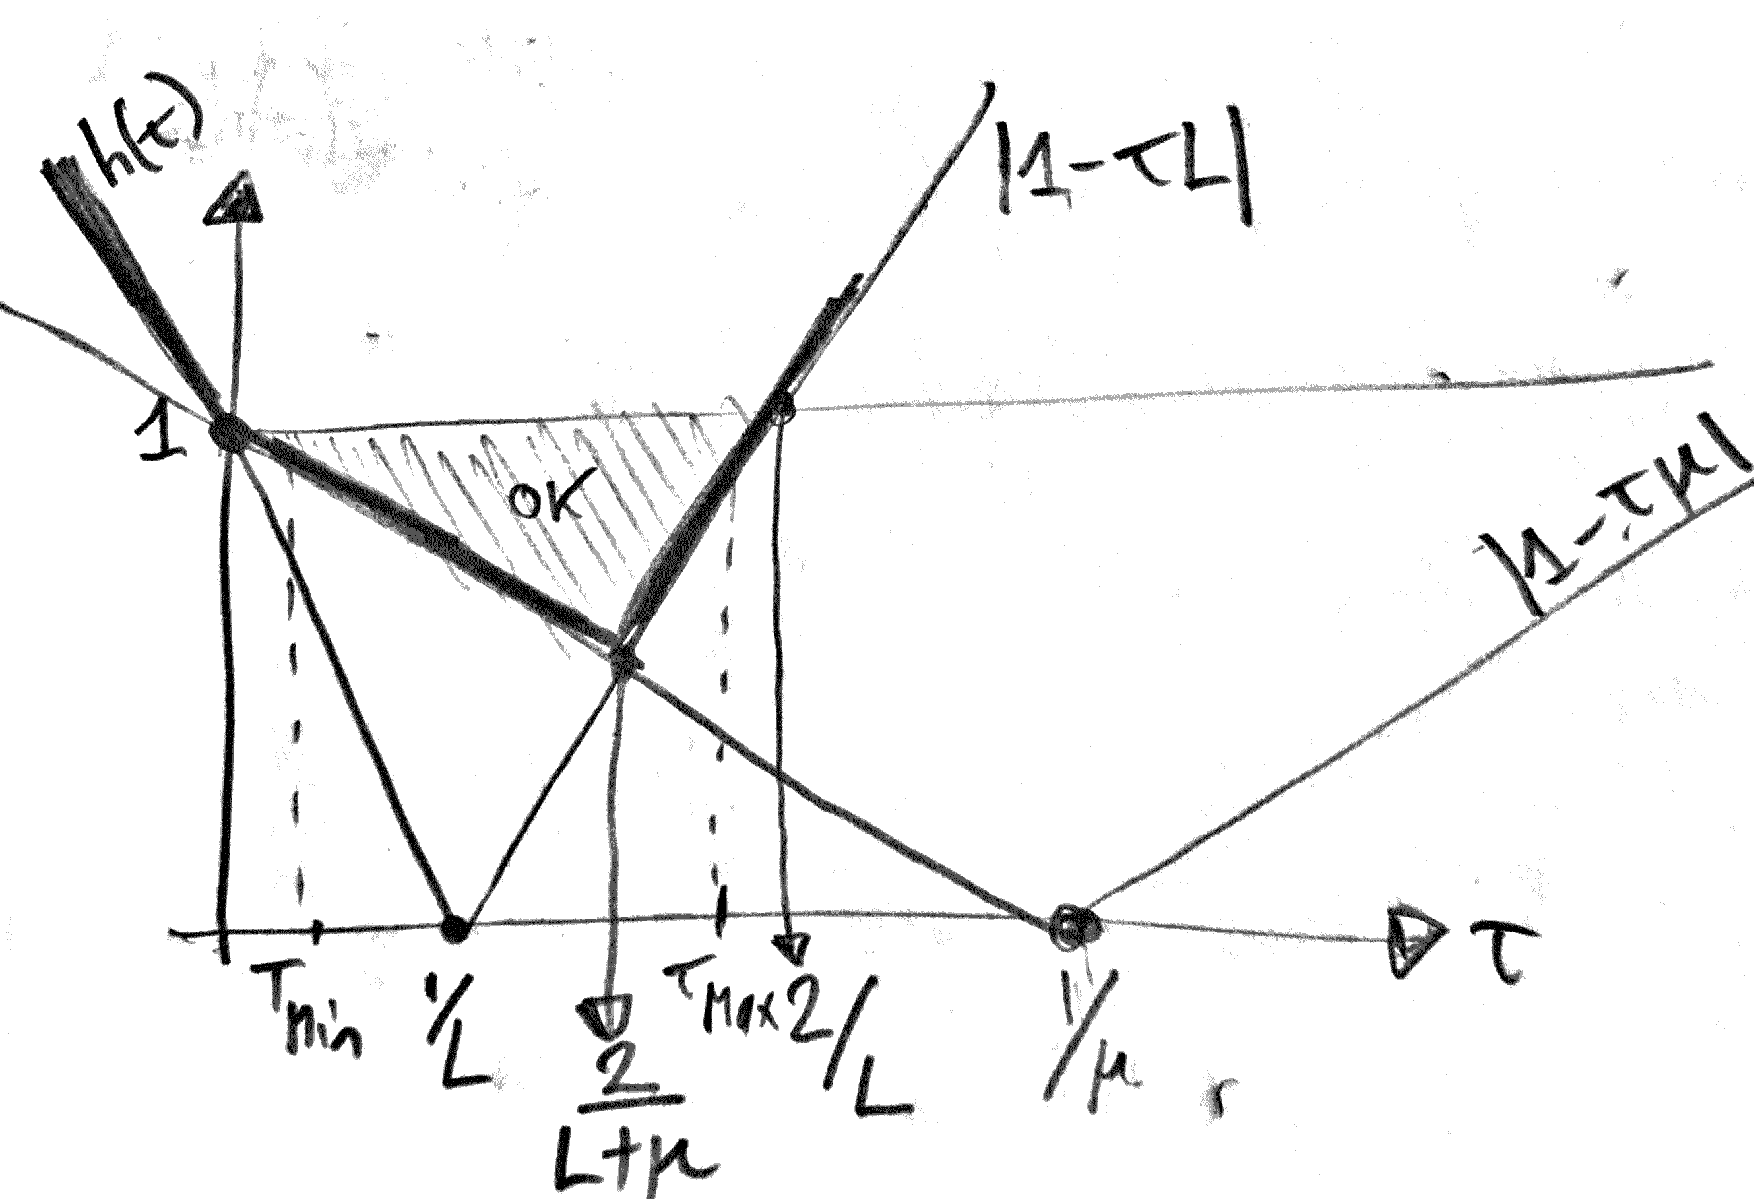
\includegraphics[width=.35\linewidth]{optim-smooth/proof-quadr}
\caption{\label{fig-grad-desc-contract}
Contraction constant $h(\tau)$ for a quadratic function (right). 
}
\end{figure}

Note that when the condition number $\xi \eqdef \mu/L \ll 1$
is small (which is the typical setup for ill-posed problems), then the contraction constant appearing in~\eqref{eq-best-rate-local} scales like 
\eql{\label{eq-rate-strong-quad}
	\tilde\rho \sim 1-2\xi.
}
%
The quantity $\epsilon$ in some sense reflects the inverse-conditioning of the problem. For quadratic function, it indeed corresponds exactly to the inverse of the condition number (which is the ratio of the largest to smallest singular value). The condition number is minimum and equal to $1$ for orthogonal matrices.

The error decay rate~\eqref{eq-global-linrate-grad}, although it is geometrical $O(\rho^k)$ is called a ``linear rate'' in the optimization literature. It is a ``global'' rate because it hold for all $k$ (and not only for large enough $k$).

If $\ker(A) \neq \{0\}$, then $C$ is not definite positive (some of its eigenvalues vanish), and the set of solution is infinite. 
%
One can however still show a linear rate, by showing that actually the iterations $x_k$ are orthogonal to $\ker(A)$ and redo the above proof replacing $\mu$ by the smaller non-zero eigenvalue of $C$. This analysis however leads to a very poor rate $\rho$ (very close to 1) because $\mu$ can be arbitrary close to 0. Furthermore, such a proof does not extends to non-quadratic functions. It is thus necessary to do a different theoretical analysis, which only shows a sublinear rate on the objective function $f$ itself rather than on the iterates $x_k$.  

\begin{prop}\label{prop-graddesc-quad-sublin}
	For $f(x)=\dotp{Cx}{x}-\dotp{b}{x}$, assuming the eigenvalue of $C$ are bounded by $L$, then if $0<\tau_k=\tau < 1/L$ is constant, then
	\eq{
		f(x_k)-f(x^\star) \leq \frac{\text{\upshape dist}(x_0,\argmin f)^2}{\tau 8 k}.
	}
	where 
	\eq{
		\text{\upshape dist}(x_0,\argmin f) \eqdef \umin{x^\star \in \argmin f} \norm{x_0-x^\star}.
	}
\end{prop}
\begin{proof}	
	We have $C x^\star=b$ for any minimizer $x^\star$
	and $x_{k+1}=x_k-\tau (C x_k-b)$ so that as before
	\eq{
		x_k-x^\star = (\Id_p-\tau C)^k(x_0-x^\star).
	}
	Now one has
	\eq{
		\frac{1}{2}\dotp{C(x_k-x^\star)}{x_k-x^\star} = 
		\frac{1}{2}\dotp{Cx_k}{x_k} 
		- \dotp{Cx_k}{x^\star}
		+ \frac{1}{2} \dotp{Cx^\star}{x^\star}
	}
	and we have $\dotp{Cx_k}{x^\star} = \dotp{x_k}{Cx^\star} = \dotp{x_k}{b}$
	and also $\dotp{Cx^\star}{x^\star} = \dotp{x^\star}{b}$ so that
	\eq{
		\frac{1}{2}\dotp{C(x_k-x^\star}{x_k-x^\star} = 
		\frac{1}{2}\dotp{Cx_k}{x_k} - \dotp{x_k}{b}
		+ \frac{1}{2} \dotp{x^\star}{b}
		= f(x_k)+ \frac{1}{2} \dotp{x^\star}{b}. % -f(x^\star)
	}
	Note also that 
	\eq{
		f(x^\star) = \frac{1}{2}\frac{Cx^\star}{x^\star} - \dotp{x^\star}{b} = \frac{1}{2}\dotp{x^\star}{b} -\dotp{x^\star}{b}  = -\frac{1}{2}\dotp{x^\star}{b}.
	}
	This shows that 
	\eq{
		\frac{1}{2}\dotp{C(x_k-x^\star}{x_k-x^\star} =f(x_k)-f(x^\star).
	}
	This thus implies 
	\eq{
		f(x_k)-f(x^\star) = 
		\frac{1}{2}\dotp{(\Id_p-\tau C)^k C (\Id_p-\tau C)^k (x_0-x^\star)}{x_0-x^\star}
		\leq \frac{\si_{\max}(M_k)}{2}  \norm{x_0-x^\star}^2
	}
	where we have denoted
	\eq{
		M_k \eqdef (\Id_p-\tau C)^k C (\Id_p-\tau C)^k.
	}
	Since $x^\star$ can be chosen arbitrary, one can replace $\norm{x_0-x^\star}$ by $\text{\upshape dist}(x_0,\argmin f)$.
	%
	One has, for any $\ell$, the following bound 
	\eq{
		\si_\ell(M_k) = \si_\ell(C) (1-\tau \si_\ell(C))^{2k}
			\leq \frac{1}{\tau 4 k}
	}
	since one can show that (setting $t = \tau \si_\ell(C) \leq 1$ because of the hypotheses)
	\eq{
		\foralls t \in [0,1], \quad
			(1-t)^{2k} t \leq \frac{1}{4k}.
	}
	Indeed, one has
	\begin{align*}
		(1-t)^{2k} t \leq (e^{-t})^{2k}t
		= \frac{1}{2k} (2kt) e^{-2k t}
		\leq \frac{1}{2k} \usup{u \geq 0} u e^{-u}
		= \frac{1}{2e k} \leq \frac{1}{4k}.
	\end{align*}
\end{proof}	
	



%%%%%%%%%%%%%%%%%%%%%%%%%%%%%%%%%%%%%%%%%%%%%%%%%%%%%%%%%%%%%%%%%%%%%%%%%%%%%%%%%%
\subsection{General Case}

We detail the theoretical analysis of convergence for general smooth convex functions. 
%
The general idea is to replace the linear operator $C$ involved in the quadratic case by the second order derivative (the hessian matrix).  

%%%
\paragraph{Hessian.}

If the function is twice differentiable along the axes, the hessian matrix is 
\eq{
	(\partial^2 f)(x) = \pa{ \frac{\partial^2 f(x)}{\partial x_i \partial x_j} }_{1 \leq i,j \leq p} \in \RR^{p \times p}.
}	
Where recall that $\frac{\partial^2 f(x)}{\partial x_i \partial x_j}$ is the differential along direction $x_j$ of the function $x \mapsto \pd{f(x)}{x_i}$. We also recall that $\frac{\partial^2 f(x)}{\partial x_i \partial x_j} = \frac{\partial^2 f(x)}{\partial x_j \partial x_i}$ so that $\partial^2 f(x)$ is a symmetric matrix.

A differentiable function $f$ is said to be twice differentiable at $x$ if
\eql{\label{eq-taylor-hess}
	f(x+\epsilon) = f(x) + \dotp{\nabla f(x)}{\epsilon} + \frac{1}{2} \dotp{\partial^2 f(x) \epsilon}{\epsilon}
	+ o(\norm{\epsilon}^2).
}
This means that one can approximate $f$ near $x$ by a quadratic function. 
%
The hessian matrix is uniquely determined by this relation, so that if one is able to write down an expansion with some matrix $H$
\eq{
	f(x+\epsilon) = f(x) + \dotp{\nabla f(x)}{\epsilon} + \frac{1}{2} \dotp{H \epsilon}{\epsilon}
	+ o(\norm{\epsilon}^2).
}
then equating this with the expansion~\eqref{eq-taylor-hess} ensure that $\partial^2 f(x)=H$. This is thus a way to actually determine the hessian without computing all the $p^2$ partial derivative.
%
This Hessian can equivalently be obtained by performing an expansion (i.e. computing the differential) of the gradient since
\eq{
	\nabla f(x+\epsilon) = \nabla f(x) + [\partial^2 f(x)](\epsilon) + o(\norm{\epsilon})
}
where $[\partial^2 f(x)](\epsilon) \in \RR^p$ denotes the multiplication of the matrix $\partial^2 f(x)$ with the vector $\epsilon$. 

One can show that a twice differentiable function $f$ on $\RR^p$ is convex if and only if for all $x$ the symmetric matrix $\partial^2 f(x)$ is positive semi-definite, i.e. all its eigenvalues are non-negative. 
% 
Furthermore, if these eigenvalues are strictly positive then $f$ is strictly convex (but the converse is not true, for instance $x^4$ is strictly convex on $\RR$ but its second derivative vanishes at $x=0$). 

For instance, for a quadratic function $f(x)=\dotp{C x}{x} - \dotp{x}{u}$, one has $\nabla f(x) = Cx-u$ and thus $\partial^2 f(x) = C$ (which is thus constant).
%
For the classification function, one has 
\eq{
	\nabla f(x) = -A^\top \diag(y) \nabla L( -\diag(y) Ax). 
}
and thus
\begin{align*}
	\nabla f(x+\epsilon) &= -A^\top \diag(y) \nabla L( -\diag(y) Ax - -\diag(y) A\epsilon)  \\
		&= \nabla f(x)  -A^\top \diag(y) [\partial^2 L( -\diag(y) Ax)]( -\diag(y) A\epsilon) 
\end{align*}
Since $\nabla L(u) = (\ell'(u_i))$ one has $\partial^2 L(u)=\diag(\ell''(u_i))$. This means that 
\eq{
	\partial^2 f(x) = A^\top \diag(y) \times \diag( \ell''(-\diag(y) Ax) ) \times \diag(y) A.
}
One verifies that this matrix is symmetric and positive if $\ell$ is convex and thus $\ell''$ is positive. 

\begin{rem}[Second order optimality condition]
The first use of Hessian is to decide wether a point $x^\star$ with $\nabla f(x^\star)$ is a local minimum or not. Indeed, if $\partial^2 f(x^\star)$ is a positive matrix (i.e. its eigenvalues are strictly positive), then $x^\star$ is a strict local minimum. 
%
Note that if $\partial^2 f(x^\star)$ is only non-negative (i.e. some its eigenvalues might vanish) then one cannot deduce anything (such as for instance $x^3$ on $\RR$). 
%
Conversely, if $x^\star$ is a local minimum then $\partial^2 f(x)$
\end{rem}

\begin{rem}[Second order algorithms]
A second use, is to be used in practice to define second order method (such as Newton's algorithm), which converge faster than gradient descent, but are more costly. The generalized gradient descent reads
\eq{
	x_{k+1} = x_k - H_k \nabla f(x_k)
}
where $H_k \in \RR^{p \times p}$ is a positive symmetric matrix. One recovers the gradient descent when using $H_k=\tau_k \Id_p$, and Newton's algorithm corresponds to using the inverse of the Hessian $H_k=[\partial^2 f(x_k)]^{-1}$.
%
Note that
\eq{
	f(x_k) = f(x_k) - \dotp{H_k \nabla f(x_k)}{\nabla f(x_k)} + o(\norm{H_k \nabla f(x_k)}).
}
Since $H_k$ is positive, if $x_k$ is not a minimizer, i.e. $\nabla f(x_k) \neq 0$, then $\dotp{H_k \nabla f(x_k)}{\nabla f(x_k)}>0$.
%
So if $H_k$ is small enough one has a valid descent method in the sense that $f(x_{k+1}) < f(x_k)$.
%
It is not the purpose of this chapter to explain in more detail these type of algorithm.
\end{rem}

The last use of Hessian, that we explore next, is to study theoretically the convergence of the gradient descent. One simply needs to replace the boundedness of the eigenvalue of $C$ of a quadratic function by a boundedness of the eigenvalues of $\partial^2 f(x)$ for all $x$.
%
Roughly speaking, the theoretical analysis of the gradient descent for a generic function is obtained by applying this approximation and using the proofs of the previous section.


%%%
\paragraph{Smoothness and strong convexity.}

\wrapfSimple{optim-smooth/up-low-bounds}
One also needs to quantify the smoothness of $f$. This is enforced by requiring that the gradient is $L$-Lipschitz, i.e.
\eql{\label{eq-lipsch-grad}\tag{$\Rr_L$}
	\foralls (x,x') \in (\RR^p)^2, \quad
	\norm{ \nabla f(x)-\nabla f(x') } \leq L \norm{x-x'}. 
}
In order to obtain fast convergence of the iterates themselve, it is needed that the function has enough ``curvature'' (i.e. is not too flat), which corresponds to imposing that $f$ is $\mu$-strongly convex
\eql{\label{eq-strong-conv}\tag{$\Ss_\mu$}
	\foralls (x,x'), \in (\RR^p)^2, \quad
	\dotp{\nabla f(x)-\nabla f(x')}{ x-x' } \geq \mu \norm{x-x'}^2. 
}
The following proposition express these conditions as constraints on the hessian for $\Cc^2$ functions.

\begin{prop}\label{prop-smooth-strong}
Conditions~\eqref{eq-lipsch-grad} and~\eqref{eq-strong-conv} imply
\eql{\label{eq-above-below-quad}
	\foralls (x,x'), \quad
	f(x') + \dotp{\nabla f(x)}{x'-x} + \frac{\mu}{2}\norm{x-x'}^2
	\leq
	f(x) 
	\leq 
	f(x') + \dotp{\nabla f(x')}{x'-x} + \frac{L}{2}\norm{x-x'}^2.
}
If $f$ is of class $\Cc^2$, conditions~\eqref{eq-lipsch-grad} and~\eqref{eq-strong-conv} are equivalent to
\eql{\label{eq-upper-lower-bound-hess}
	\foralls x, \quad \mu \Id_{p}  \preceq \partial^2 f(x) \preceq L \Id_{p}
}
where $\partial^2 f(x) \in \RR^{p \times p}$ is the Hessian of $f$, and 
where $\preceq$ is the natural order on symmetric matrices, i.e.
\eq{
	A \preceq B \quad\Longleftrightarrow\quad
	\foralls x \in \RR^p, \quad \dotp{A u}{u} \leq \dotp{B u}{u}.
}
\end{prop}

\begin{proof}
	We prove~\eqref{eq-above-below-quad}, using Taylor expansion with integral remain
	\eq{
		f(x') - f(x) = \int_0^1 \dotp{\nabla f(x_t)}{x'-x} \d t
		= \dotp{\nabla f(x)}{x'-x} + \int_0^1 \dotp{\nabla f(x_t)-\nabla f(x)}{x'-x} \d t		
	}
	where $x_t \eqdef x+t(x'-x)$.
	%
	Using Cauchy-Schwartz, and then the smoothness hypothesis~\eqref{eq-lipsch-grad}
	\eq{
		f(x') - f(x) \leq \dotp{\nabla f(x)}{x'-x} +  \int_0^1 L \norm{x_t-x} \norm{x'-x} \d t
		\leq \dotp{\nabla f(x)}{x'-x} +  L \norm{x'-x}^2 \int_0^1  t  \d t
	} 
	which is the desired upper-bound. Using directly~\eqref{eq-strong-conv} gives 
	\eq{
		f(x') - f(x) 
		= \dotp{\nabla f(x)}{x'-x} + \int_0^1 \dotp{\nabla f(x_t)-\nabla f(x)}{\frac{x_t-x}{t}} \d t	
		\geq \dotp{\nabla f(x)}{x'-x} + \mu \int_0^1 \frac{1}{t}\norm{x_t-x}^2  \d t
	}
	which gives the desired result since $\norm{x_t-x}^2 / t = t \norm{x'-x}^2$.
\end{proof}

The relation~\eqref{eq-above-below-quad} shows that a smooth (resp. strongly convex) functional is bounded by below (resp. above) by a quadratic tangential majorant (resp. minorant). 

Condition~\eqref{eq-upper-lower-bound-hess} thus reads that the singular values of $\partial^2 f(x)$ should be contained in the interval $[\mu,L]$. The upper bound is also equivalent to $\norm{\partial^2 f(x)}_{\text{op}} \leq L$ where $\norm{\cdot}_{\text{op}}$ is the operator norm, i.e. the largest singular value. 
%
In the special case of a quadratic function of the form $\dotp{Cx}{x}-\dotp{b}{x}$ (recall that necessarily $C$ is semi-definite symmetric positive for this function to be convex), $\partial^2 f(x)=C$ is constant, so that $[\mu,L]$ can be chosen to be the range of the eigenvalues of $C$.

%%%
\paragraph{Convergence analysis.}

We now give convergence theorem for a general convex function. On contrast to quadratic function, if one does not assumes strong convexity, one can only show a sub-linear rate on the function values (and no rate at all on the iterates themselves). It is only when one assume strong convexity that linear rate is obtained. 
%
Note that in this case, the solution of the minimization problem is not necessarily unique.

\begin{thm}\label{thm-gradsec-non-strong-conv}
	If $f$ satisfy conditions~\eqref{eq-lipsch-grad}, assuming there exists $(\tau_{\min},\tau_{\max})$ such that
	\eq{
		0 < \tau_{\min} \leq \tau_\ell \leq \tau_{\max} < \frac{2}{L}, 
	}
	then $x_k$ converges to a solution $x^\star$ of~\eqref{eq-general-pbm} and
	there exists $C>0$ such that 
	\eql{\label{eq-sublin-rate-gd}
		f(x_k)-f(x^\star) \leq \frac{C}{\ell+1}.
	} 
	If furthermore $f$ is $\mu$-strongly convex, then there exists $0 \leq \rho < 1$ such that $\norm{x_k-x^\star} \leq \rho^\ell \norm{x_0-x^\star}$.
\end{thm}

\begin{proof}
	In the case where $f$ is not strongly convex, we only prove~\eqref{eq-sublin-rate-gd} since the proof that $x_k$ converges is more technical. Note indeed that if the minimizer $x^\star$ is non-unique, then it might be the case that the iterate $x_k$ ``cycle'' while approaching the set of minimizer, but actually convexity of $f$ prevents this kind of pathological behavior. 
	%
	For simplicity, we do the proof in the case $\tau_\ell = 1/L$, but it extends to the general case. 
	%
	The $L$-smoothness property imply~\eqref{eq-above-below-quad}, which reads
	\eq{
	f(x_{k+1}) 
		\leq 
		f(x_k) + \dotp{\nabla f(x_k)}{x_{k+1}-x_k} + \frac{L}{2}\norm{x_{k+1}-x_k}^2.
	}
	Using the fact that $x_{k+1}-x_k = -\frac{1}{L} \nabla f(x_k)$, one obtains
	\eql{\label{eq-proox-x'rad-nonstrong-1}
		f(x_{k+1}) 
		\leq 
		f(x_k) -  \frac{1}{L} \norm{\nabla f(x_k)}^2 + \frac{1}{2L} \norm{\nabla f(x_k)}^2
		\leq  f(x_k) -  \frac{1}{2L} \norm{\nabla f(x_k)}^2 
	}
	This shows that $(f(x_k))_\ell$ is a decaying sequence.
	%
	By convexity
	\eq{
		f(x_k) + \dotp{\nabla f(x_k)}{x^\star-x_k} \leq f(x^\star)
	}
	and plugging this in~\eqref{eq-proox-x'rad-nonstrong-1} shows
	\begin{align}
		f(x_{k+1})  &\leq   
		f(x^\star) - \dotp{\nabla f(x_k)}{x^\star-x_k} - \frac{1}{2L} \norm{\nabla f(x_k)}^2 \\
		&= f(x^\star) + \frac{L}{2}\pa{
			\norm{x_k-x^\star}^2 - \norm{x_k-x^\star-\frac{1}{L}\nabla f(x_k)}^2
		}\\
		&= f(x^\star) + \frac{L}{2}\pa{
			\norm{x_k-x^\star}^2 - \norm{x^\star-x_{k+1}}^2 }. \label{eq-conv-rate-proof-1}
	\end{align}
	Summing these inequalities for $\ell=0,\ldots,k$, one obtains
	\eq{
		\sum_{\ell=0}^k f(x_{k+1}) - (k+1) f(x^\star) \leq  \frac{L}{2}\pa{
			\norm{x_0-x^\star}^2 - \norm{x^{(k+1)}-x^\star}^2 }
	}
	and since $f(x_{k+1})$ is decaying $\sum_{\ell=0}^k f(x_{k+1}) \geq (k+1) f(x^{(k+1)})$, thus 
	\eq{
		f(x^{(k+1)}) - f(x^\star) \leq \frac{L \norm{x_0-x^\star}^2}{2(k+1)}
	}
	which gives~\eqref{eq-sublin-rate-gd} for $C \eqdef L \norm{x_0-x^\star}^2/2$.
	
	If we now assume $f$ is $\mu$-strongly convex, then, using $\nabla f(x^\star)=0$, one has $\frac{\mu}{2}\norm{x^\star-x}^2 \leq f(x)-f(x^\star)$ for all $x$. 
	%
	Re-manipulating~\eqref{eq-conv-rate-proof-1} gives
	\eq{
		\frac{\mu}{2}\norm{ x_{k+1} - x^\star}^2 \leq f(x_{k+1})-f(x^\star) \leq \frac{L}{2}\pa{
			\norm{x_k-x^\star}^2 - \norm{x^\star-x_{k+1}}^2 }, 
	}
	and hence
	\eql{\label{eq-rate-strong}
		\norm{ x_{k+1} - x^\star} \leq \sqrt{ \frac{L}{L+\mu} } \norm{ x_{k+1} - x^\star}, 
	}
	which is the desired result. 
\end{proof}

Note that in the low conditioning setting $\epsilon \ll 1$, one retrieve a dependency of the rate~\eqref{eq-rate-strong} similar to the one of quadratic functions~\eqref{eq-rate-strong-quad}, indeed 
\eq{
	\sqrt{ \frac{L}{L+\mu} } = (1+\epsilon)^{-\frac{1}{2}} \sim 1 - \frac{1}{2}\epsilon. 
}


%%%%%%%%%%%%%%%%%%%%%%%%%%%%%%%%%%%%%%%%%%%%%%%%%%%%%%%%%%%%%%%%%%%%%%%%%%%%%%%%%%
\subsection{Acceleration}

The previous analysis shows that for $L$-smooth functions (i.e. with a hessian uniformly bounded by $L$, $\norm{\partial^2 f(x)}_{\text{op}} \leq L$), the gradient descent with fixed step size converges with a speed on the function value $f(x_k)-\min f = O(1/k)$. 
%
Even using various line search strategies, it is not possible to improve over this rate. 
%
A way to improve this rate is by introducing some form of ``momentum'' extrapolation and rather consider a pair of variables $(x_k,y_k)$ with the following update rule, for some step size $s$ (which should be smaller than $1/L$)
\eq{
	\choice{
			x_{k+1} = y_{k} - s \nabla f(y_{k}) \\
			y_{k+1} = x_{k+1} + \beta_k (x_{k+1}-x_{k})
	}
}
where the extrapolation parameter satisfies $0 < \beta_k < 1$. The case of a fixed $\beta_k=\be$ corresponds to the so-called ``heavy-ball'' method. In order for the method to bring an improvement for the $1/k$ ``worse case'' rate (which does not means it improves for all possible case), one needs to rather use increasing momentum $\beta_k \rightarrow 1$, one popular choice being
\eq{
	\be_k \frac{k-1}{k+2} \sim 1 - \frac{1}{k} .
}
This corresponds to the so-called ``Nesterov'' acceleration (although Nesterov used a slightly different choice, with the similar $1-1/k$ asymptotic behavior).

When using $s \leq 1/L$, one can show that $f(x_k)-\min f = O( \frac{\norm{x_0-x^\star}}{s k^2} )$, so that in the worse case scenario, the convergence rate is improved. Note however that in some situation, acceleration actually deteriorates the rates. For instance, if the function is strongly convex (and even on the simple case $f(x)=\norm{x}^2$), Nesterov acceleration does not enjoy linear convergence rate.

A way to interpret this scheme is by looking at a time-continuous ODE limit when $s \rightarrow 0$. On the contrary to the classical gradient descent, the step size here should be taker as $\tau=\sqrt{s}$ so that the time evolves as $t=\sqrt{s} k$. 
% 
The update reads
\eq{
	\frac{x_{k+1} - x_k}{\tau} = (1-3/k) \frac{x_k-x_{k-1}}{\tau} -  \nabla f(y_k)
}
which can be re-written as
\eq{
	\frac{x_{k+1}+x_{k-1} - 2 x_k}{\tau^2} - \frac{3}{k\tau} \frac{x_k-x_{k-1}}{\tau} + \tau \nabla f(y_k) = 0.
}
Assuming $(x_k,y_k) \rightarrow (x(t), y(t))$, one obtains in the limit the following second order ODE
\eq{
	x''(t) + \frac{3}{t} x'(t) + \nabla f(x(t)) = 0
	\qwithq
	\choice{
		x(0)=x_0, \\
		x'(0)=0.
	}
}
This corresponds to the movement of a ball in the potential field $f$, where the term $\frac{3}{t} x'(t)$ plays the role of a friction which vanishes in the limit.
%
So for small $t$, the method is similar to a gradient descent $x'=-\nabla f(x)$, while for large $t$, it ressemble a Newtonian evolution $x''=-\nabla f(x)$ (which keeps oscillating without converging). 
%
The momentum decay rate $3/t$ is very important, it is the only rule which enable the speed improvement from $1/k$ to $1/k^2$.
% !TEX root = ../optim-ml/MirrorDescent.tex

%%%%%%%%%%%%%%%%%%%%%%%%%%%%%%%%%%%%%%%%%%%%%%%%%%%%%%%%%%%%%%%%%%%%%%%%%%%%%%%%%%
%%%%%%%%%%%%%%%%%%%%%%%%%%%%%%%%%%%%%%%%%%%%%%%%%%%%%%%%%%%%%%%%%%%%%%%%%%%%%%%%%%
%%%%%%%%%%%%%%%%%%%%%%%%%%%%%%%%%%%%%%%%%%%%%%%%%%%%%%%%%%%%%%%%%%%%%%%%%%%%%%%%%%
\section{Mirror Descent and Implicit Bias}


%%%%%%%%%%%%%%%%%%%%%%%%%%%%%%%%%%%%%%%%%%%%%%%%%%%%%%%%%%%%%%%%%%%%%%%%
\subsection{Bregman Divergences}

We consider a smooth strictly convex ``entropy'' function $\psi$ such that $\norm{\nabla \psi(x)}$ goes to $+\infty$ as $x \rightarrow \partial \dom(\psi)$.
%
We denote 
\eq{
	\psi^*(u) \eqdef \usup{x \in \dom(\psi)} \dotp{u}{x} - \psi(x)
}
its Legendre transform.
%
In this case of ``Legendre-type'' entropy function, $\nabla\psi : \dom(\psi) \rightarrow \dom(\psi^\star)$ and $\nabla\psi^*$ are bijection reciprocal one from the other.

One then defines the associated Bregman divergence
\eq{
	\BregD_\psi(x|y) \triangleq \psi(x)-\psi(y) - \dotp{\nabla\psi(y)}{x-y}.
}
It is positive, convex in $x$ (but not necessarily in $y$), not necessarily symmetric, and ``distance-like''.

For $\psi=\norm{\cdot}^2$ one has $\nabla\psi=\nabla\psi^*=\Id$, and one recovers the Euclidean distance. 
%
For $\psi_{\KL}(x)=\sum_i x_i \log(x_i)-x_i+1$ one has $\nabla\psi=\log$ and $\nabla\psi^*=\exp$, and one obtains the relative entropy, also known as Kullback-Leibler 
\eq{
	\BregD_{\psi_{\KL}}(x|y) = \sum_{i} x_i \log(x_i/y_i)-x_i+y_i.
}
%
When $\psi_{\text{Burg}}(x)=\sum_i -\log(x_i)+x_i-1$ on $\RR_+^d$, $\nabla \psi_{\text{Burg}}(x)=\nabla\psi^*(x)=-1/x$ and associated divergence 
\eql{\label{eq-burg-entropy}
	\BregD_{\psi_{\text{Burg}}}(x|y) = \sum_i -\log(y_i/x_i) - x_i/y_i+1.
}


These examples can be generalized to power entropies
\eql{\label{eq-power-entropies}
	\psi_\al(x) \triangleq \sum_i \frac{|x_i|^\al-\al (x_i-1)-1}{\al (\al-1)}
}
with special cases
\eq{
	\psi_1(x) \triangleq \psi_{\KL} = \sum_i x_i \log(x_i)-x_i+1
	\qandq 
	\psi_0(x) \triangleq \psi_{\text{Burg}} = \sum_i -\log(x_i)+x_i-1.
}
They are defined on $\RR^d$ if $\al>1$ and $\RR_+^d$ if $\al \leq 1$. 

\begin{rem}[Matricial divergences]
	Given an entropy function $\psi_0(x)$ on vectors $x \in \RR^d$ which is invariant under permutation of the indices, one lifts it to symmetric matrices $X \in \RR^{d \times d}$ as
	\eq{
		\psi(X) \triangleq \psi_0(\La(X)) \qwhereq 
		X = U_X \diag(\La(X)) U_X^\top
	}
	is the eigen-decomposition of $X$, where $\La(X) = (\la_i(X))_{i=1}^d \in \RR^d$ are the eigenvalues. Typically, if $\psi_0(x)=\sum_i h(x_i)$ then $\psi(X)=\tr(h(X))$ where $h$ is extended to matrices as $h(X) \triangleq U_X \diag(h(\la_i(X))) U_X^\top$. If $\psi_0$ is convex and smooth, so is $\psi$, and 
	\eq{
		\nabla \psi(X) = U_X \diag(\nabla \psi_0(\La(X))) U_X^\top. 
	} 
	For instance, if $h(s)=s\log(x)-s+1$ is the Shannon entropy, this defines the quantum Shannon entropy as
	\eq{
		\BregD_\psi(X) = \tr(X \log(X)-X \log(Y)-X+Y)
	}
	and if $h(s)=-\log(s)$ then $\BregD_\psi(X)=-\log\det(X)$.
\end{rem}

\begin{rem}[Cizard divergences]
When defined on $\RR_+^d$, these divergence should not be confounded with Cizar divergences which reads
\eq{
	\text{C}_{\psi}(x|y) \eqdef \sum_{i} y_i \psi(x_i/y_i) + \psi'_\infty  \sum_{y_i=0} x_i, 
}
which are jointly convex in $x$ and $y$. 
%
Only for $\psi=\psi_{\KL}$ one has $\BregD_{\psi_{\KL}} = \text{C}_{\psi_{\KL}}$. 
\end{rem}

%%%%%%%%%%%%%%%%%%%%%%%%%%%%%%%%%%%%%%%%%%%%%%%%%%%%%%%%%%%%%%%%%%%%%%%%
\subsection{Mirror descent}

We consider the following implicit stepping 
\eq{
	x_{k+1} = \uargmin{x \in \dom(\psi)} f(x) + \frac{1}{\tau} \BregD_\psi(x|x_k).
}
Its explicit version then reads by Taylor expanding $f$ at $x_k$
\begin{align*}
     x_{k+1} &= \uargmin{x \in \dom(\psi)} f(x_k) + \dotp{x-x_k}{\nabla f(x_k)} + \frac{1}{\tau} \BregD_\psi(x|x_k), \\
     	&= \uargmin{x \in \dom(\psi)} \dotp{x}{\nabla f(x_k)} + \frac{1}{\tau} \BregD_\psi(x|x_k).
\end{align*}
The fact that $\psi$ is Legendre type allows to ignore the constraint, and the solution satisfies the following first order condition
\eq{
	\nabla f(x_k) + 1/\tau  [ \nabla \psi(x_{k+1}) -  \nabla \psi(x_k)] = 0
}
so that it can be explicitly computed      
\eql{\label{eq-mirror-descent}
    x_{k+1} = (\nabla \psi^*)[  \nabla \psi(x_k) - \tau \nabla f(x_k)  ]
}
For $\psi=\norm{\cdot}^2/2$ one recovers the usual Euclidean gradient descent.
%
For $\psi(x)=\sum_i x_i \log(x_i)$, this defines the multiplicative updates
\eq{
     x_{k+1} = x_k \odot \exp( -\tau \nabla f(x_k) )
}
where $\odot$ is the entry-wise multiplication of vectors.

Note that introducing the ``dual'' variable $u_k \triangleq \nabla \psi(x_k)$, one has
\eql{\label{eq-mirror-dual}
	u_{k+1} = u_k - \tau h(u_k) \qwhereq 
	h(u) \triangleq  \nabla f(\nabla \psi^*(u)).  
}
Note however that in general $h$ is not a gradient field, so this is not in general a gradient flow.

%%%%
\paragraph{Mirror flow.}

When $\tau \to 0$, one obtains the following expansion
\eq{
    x_{k+1} = (\nabla \psi^*)[\nabla \psi(x_k)] - \tau  [\partial^2 \psi^*]( \nabla \psi(x_k) )  \times \nabla f(x_k)  + o(\tau)
}
so that defining $x(t)=x_{k}$ for $t=k \tau$ the limit is the following flow
\eql{\label{eq-hessian-flow}     
	\dot x(t) = -H(x(t)) \nabla f(x(t))
	\qwhereq
        H(x) \triangleq [\partial^2 \psi^*]( \nabla \psi(x) ) = [\partial^2 \psi(x)]^{-1}
 }
 so that this is a gradient flow on a very particular type of manifold, of ``Hessian type''.
%
Note that if $\psi=f$, then one recovers the flow associated to Newton's method.

%%%%
\paragraph{Convergence.}

Convergence theory (ensuring convergence and rates) for mirror descent is the same as for the usual gradient descent, and one needs to consider relative $L$-smoothness, and if possible also relative $\mu$-strong  convexity, 
\eq{
	\mu \BregD_\psi \leq \BregD_f \leq L \BregD_\psi
	\quad\Longleftrightarrow\quad
	\foralls x, \: \mu \partial^2 \psi(x) \leq \partial^2 f(x)  \leq L \partial^2 \psi(x) .
}
If $L<+\infty$, then one has $f(x_k)-f(x^\star) \leq O( \BregD_\psi(x^\star|x_0)/k)$
while if both $0<\mu \leq L <+\infty$, then $\BregD_\psi(x_k|x^\star) \leq O( \BregD_\psi(x^\star|x_0) (1-\mu/L)^k)$.
%
The advantages of using Bregman geometry are two-fold: this can improves the conditioning $\mu/L$ (some function might be non-smooth for the Euclidean geometry but smooth for some Bregman geometry, and can avoid introducing constraint in the optimization problem) and this can also lower the radius of the domain  $\BregD_\psi(x^\star|x_0)$. 
%
For instance, assuming the solution belongs to the simplex, and using $x_0=\ones_d/d$, then $\BregD_{\psi_{\KL}}(x^\star|x_0) \leq \log(d)$ whereas for the $\ell^2$ Euclidean distance, one only has the bound $\norm{x^\star-x_0}^2 \leq d$.


%%%%%%%%%%%%%%%%%%%%%%%%%%%%%%%%%%%%%%%%%%%%%%%%%%%%%%%%%%%%%%%%%%%%%%%%
\subsection{Re-parameterized flows}

One can consider a change of variable $x=\phi(z)$ where $\phi : \RR^p \mapsto \Xx \subset \RR^d$ is a smooth map, and perform the gradient descent on the function $g(z) \triangleq f(\phi(z))$. Then one has
\eq{
	\nabla g(z) = [\partial \phi(z)]^\top \nabla f(x)
}
so that, denoting $z(t)$ the gradient flow $\dot z=-\nabla g(z)$ of $g$, and $x(t) \triangleq \phi(z(t))$, one has
$\dot x(t) = [\partial \phi(z(t))] \dot z(t)$ and thus $x(t)$ solves the following equation
\eq{
	\dot x = -Q(z) \nabla f(x)  \qwithq 
	 Q(z) \triangleq [\partial \phi(z)] [\partial \phi(z)]^\top \in \Ss_+^{d \times d}
}
So unless $\phi$ is a bijection, this is not a gradient flow over the $x$ variable. If $\phi$ is a bijection, then this is a gradient flow associated to the field of tensors (``manifold'') $Q(\phi^{-1}(x))$. The issue is that even in this case, in general $H$ might fail to be a Hessian manifold, so this does not correspond to a mirror descent flow. 

\paragraph{Dual parameterization} 

If $\psi$ is an entropy function, then the parametrization $x=\nabla\psi^*(z)$, i.e. $\phi=\nabla\psi^*$, then 
$Q(z)=[\partial^2 \psi^*(z)]^2$, i.e. $Q(\phi^{-1}(x)) = [\partial^2 \psi(x)]^{-2}$ is not of Hessian-type in general, but rather a squared-Hessian manifold.
%
For instance, when $\psi^*(z)=\exp(z)$, then $Q(\phi^{-1}(x)) = \diag(1/x_i^2)$, which surprisingly is the hessian metric associated to Burg's entropy $-\sum_i \log(x_i)$.


\paragraph{Example: power-type parameterization}

We consider power entropies~\eqref{eq-power-entropies}, on $\RR_+^d$, for $\al \leq 1$, for which 
\eq{
	H(x)  = [\partial^2 \psi(x)]^{-1} \propto \diag( x_i^{2-\al} ).
}
%
Remark than when using the parameterization $x = \phi(z) = (z_i^{b})_i$ then  
\eq{
	Q(\phi^{-1}(x)) = [\partial \phi(z)] [\partial \phi(z)]^\top
	\propto \diag( z_i^{2(b-1)} ) = \diag( x_i^{2(b-1)/b} ) 
}
so if one selects $2(1-1/b) = 2-\al$ i.e. $2/b = \al$, the re-parameterized flow is equal to the flow on a Hessian manifold. 
%
For instance, when setting $b=2$, $\al=1$, i.e. using the parmeterization $x=z^2$, one retrieves the flow on the manifold for the Shannon entropy (``Fisher-Rao'' geometry). 
%
Note that when $b \rightarrow +\infty$, one obtains $\al=0$, i.e. the flow is the one of the Burg's entropy $\psi(x)=-\sum_i \log(x_i)$ (which we saw above as also being associated to the parameterization $x=\exp(z)$).


\paragraph{Counter-example: SDP matrices}

We now consider semi-definite symmetric matrices $X \in \Ss_+^{d \times d}$, together with the parameterization $X = \phi(Z) = ZZ^\top$ for $Z \in \RR^{d \times d}$.
%
In this case, denoting $g(Z)=f(ZZ^\top)$, one has
\eq{
	\nabla g(Z) = [\nabla f(X) + \nabla f(X)^\top] Z
}
so that the flow $\dot Z = -\nabla g(Z)$ is equivalent to the following flow on symmetric (and it maintains positivity as well)
\eql{\label{eq-flow-repar-matrices}
     \dot X = X [\nabla_S f(X)] + [\nabla_S f(X)] X
}
where the symmetric gradient is
\eq{
	\nabla_S f(X) \triangleq [\nabla f(X)] + [\nabla f(X)]^\top
}
So most likely~\eqref{eq-flow-repar-matrices} cannot be written as a usual gradient flow on a manifold which would be a hessian of a convex function. To mimic the diagonal case (or vectorial case above), the most natural quantitate would have been the spectral entropy $\psi(X) \triangleq \tr( X \log(X)-X+\Id)$,  whose gradient is $\log(X)$, but there is no closed form expression for the derivative of the log unfortunately.
%
Another simpler approach to mimic $\psi_{-1}$ is to use $\psi(X)=-\tr(\log(X))=-\log\det(X)$, because the Hessian and its inverse can be computed
\eq{
	\partial^2 \psi(X) : S \mapsto - X^{-1}SX^{-1}.
}




%%%%%%%%%%%%%%%%%%%%%%%%%%%%%%%%%%%%%%%%%%%%%%%%%%%%%%%%%%%%%%%%%%%%%%%%
\subsection{Implicit Bias}


We consider the problem
\eq{
   \umin{x \in \RR^d} f(x) = L(Ax) \triangleq \sum_i \ell( \dotp{a_i}{x},y_i),
}
where the loss is coercive such that $\ell(\cdot,y_i)$ has a unique minimizer at $y_i$. The typical example is $f(x)=\norm{Ax-y}^2$ for $\ell(u,v)=(u-v)^2$. 
%
We do not impose that $L$ is convex, and simply assumes convergence of the considered optimization method to the set of global minimizers.
%
The set of global minimizers is thus the affine space
\eq{ 
     \argmin f =  \enscond{x}{Ax=y}.
}

The simplest optimization method is just gradient descent 
\eq{
	x_{k+1} = x_k - \tau \nabla f(x_k)
	\qwhereq
	\nabla f(x) = A^\top \nabla L(Ax).
}
As $\tau \rightarrow 0$, one defines $x(t)=x_k$ for $t=k\tau$ and consider the flow
\eq{
	\dot x(t) = -\nabla f(x(t)).
}
The implicit bias of the descent (and the flow) is given by the orthogonal projection. 

\begin{prop}\label{prop-implicit-bias-l2}
	If $x_k \rightarrow x^\star \in \argmin f$, then
	\eq{
		x^\star = \uargmin{x \in \argmin f} \norm{x-x_0}.
	}
\end{prop}

The following Proposition, whose proof can be found in~\cite{gunasekar2018characterizing} generalizes this proposition to the case of an arbitrary mirror flow. 

\begin{prop}\label{prop-implicit-bias-mirror}
	If $x_k$ defined by~\eqref{eq-mirror-descent} (resp. $x(t)$ defined by~\eqref{eq-hessian-flow}) is such that $x_k$ (resp. $x(t)$) converges to $x^\star \in \argmin f$, then
	\eql{\label{eq-implicit-bias-mirror}
		x^\star = \uargmin{x \in \argmin f} \BregD_\psi(x|x_0).
	}
\end{prop}
\begin{proof} 
	From the dual variable evolution~\eqref{eq-mirror-dual}, since $\nabla f(x) \in \Im(A^\top)$, one has that $y_k-y_0 \in \Im(A^\top)$, so that in the limit 
	\eql{\label{eq-evol-dual}
		y^\star - y_0 = \nabla\psi(x^\star) - \nabla\psi(x_0) \in \Im(A^\top). 
	}
	Note that $\nabla\BregD_\psi(x|x_0) =\nabla\psi(x) - \nabla\psi(x_0)$, and $\Im(A^\top) = \Ker(A)^\bot$ is the space orthogonal to $\argmin f$ so that~\eqref{eq-evol-dual} are the optimality conditions of the strictly convex problem~\eqref{eq-implicit-bias-mirror}.
\end{proof}

In particular, for the Shannon entropy (equivalently when using the $x=z^2$ parameterization), as $x_0 \rightarrow 0$, by doing the expansion of $\KL(x|x_0)$ one has 
\eq{
		x^\star \rightarrow \uargmin{x \in \argmin f, x \geq 0} \sum_i |\log((x_0)_i)| x_i, 
}
which is a weighted $\ell^1$ norm (so in particular it induces sparsity in the solution, it is a Lasso-type problem).

When using more general parameterizations of the form $x=z^b$ for $b>0$, this corresponds to using the power entropy $\psi_\al$ for $\al = 2/b$, and one can check that the associated limit bias for small $x_0$ is still an $\ell^1$, but with a different weighting scheme. For $x=\exp(z)$ (or $b \rightarrow +\infty$) one obtains Burg's entropy defined in~\eqref{eq-burg-entropy} so that the limit bias is  $\sum_i x_i/(x_0)_i$. 
%
The use of $x=z^2$ parameterization (which can be generalized to $x=u \odot v$ for signed vectors) was introduced in~\cite{hoff2017lasso}, and its associated implicit regularization is detailed in~\cite{vavskevivcius2019implicit,zhao2019implicit}. 
%
It is possible to analyze this sparsity-inducing behavior in a quantitative way, see for instance~\cite[Thm.2]{woodworth2020kernel}
%
One can generalize this parameterization to arbitrary (not only positive vector) by using $x=u^2-v^2$ or $x=u \odot v$ and the same type of bias appears, with now rather a (weighted) $\ell^1$ norm.

% !TEX root = ../optim-ml/OptimML.tex


%%%%%%%%%%%%%%%%%%%%%%%%%%%%%%%%%%%%%%%%%%%%%%%%%%%%%%%%%%%%%%%%%%%%%%%%
%%%%%%%%%%%%%%%%%%%%%%%%%%%%%%%%%%%%%%%%%%%%%%%%%%%%%%%%%%%%%%%%%%%%%%%%
%%%%%%%%%%%%%%%%%%%%%%%%%%%%%%%%%%%%%%%%%%%%%%%%%%%%%%%%%%%%%%%%%%%%%%%%
\section{Regularization}

When the number $n$ of sample is not large enough with respect to the dimension $p$ of the model, it makes sense to regularize the empirical risk minimization problem. 


%%%%%%%%%%%%%%%%%%%%%%%%%%%%%%%%%%%%%%%%%%%%%%%%%%%%%%%%%%%%%%%%%%%%%%%%
\subsection{Penalized Least Squares}

For the sake of simplicity, we focus here on regression and consider
\eql{\label{eq-regul-ls}
	\umin{x \in \RR^p} f_\la(x) \eqdef \frac{1}{2}\norm{Ax-y}^2 + \la R(x) 
}
where $R(x)$ is the regularizer and $\la\geq 0$ the regularization parameter. 
%
The regularizer enforces some prior knowledge on the weight vector $x$ (such as small amplitude or sparsity, as we detail next) and $\la$ needs to be tuned using cross-validation.

We assume for simplicity that $R$ is positive and coercive, i.e. $R(x) \rightarrow +\infty$ as $\norm{x} \rightarrow +\infty$. 
%
The following proposition that in the small $\la$ limit, the regularization select a sub-set of the possible minimizer. This is especially useful when $\ker(A) \neq 0$, i.e. the equation $Ax=y$ has an infinite number of solutions.

\begin{prop}
	If $(x_{\la_k})_k$ is a sequence of minimizers of $f_\la$, then this sequence is bounded, and any accumulation $x^\star$ is a solution of the constrained optimization problem
	\eql{\label{eq-regul-constr}
		\umin{Ax=y} R(x).
	}
\end{prop}


\begin{proof}
	Let $x_0$ be so that $Ax_0=y$, then by optimality of $x_{\la_k}$
	\eql{\label{eq-ineq-proof-regul}
			\frac{1}{2}\norm{Ax_{\la_k}-y}^2 + \la_k R(x_{\la_k}) \leq \la_k R(x_0).
	}
	Since all the term are positive, one has $R(x_{\la_k}) \leq  R(x_0)$ so that $(x_{\la_k})_k$ is bounded by coercivity of $R$.
	%
	Then also $\norm{Ax_{\la_k}-y} \leq \la_k R(x_0)$, and passing to the limit, one obtains $Ax^\star = y$.
	%
	And passing to the limit in $R(x_{\la_k}) \leq R(x_0)$ one has $R(x^\star) \leq R(x_0)$ which shows that $x^\star$ is a solution of~\eqref{eq-regul-constr}. 
\end{proof}

%%%%%%%%%%%%%%%%%%%%%%%%%%%%%%%%%%%%%%%%%%%%%%%%%%%%%%%%%%%%%%%%%%%%%%%%
\subsection{Ridge Regression}

Ridge regression is by far the most popular regularizer, and corresponds to using $R(x)=\norm{x}^2_{\RR^p}$. Since it is strictly convex, the solution of~\eqref{eq-regul-ls} is unique
\eq{
	x_\la \eqdef \uargmin{x \in \RR^p} f_\la(x) = \frac{1}{2} \norm{Ax-y}^2_{\RR^n} + \la \norm{x}^2_{\RR^p}.
}
One has 
\eq{
	\nabla f_\la(x) = A^\top (Ax_\la - y) + \la x_\la = 0
}
so that $x_\la$ depends linearly on $y$ and can be obtained by solving a linear system. The following proposition shows that there are actually two alternate formula.

\begin{prop}
	One has
	\begin{align}
		x_\la &= (A^\top A + \la \Id_p)^{-1} A^\top y,  \label{eq-regul-ls-1} \\
			 &= A^\top (A A^\top + \la \Id_n)^{-1} y. \label{eq-regul-ls-2} 
	\end{align}
\end{prop}

\begin{proof}
	Denoting $B \eqdef (A^\top A + \la \Id_p)^{-1} A^\top$ and $C \eqdef A^\top (A A^\top + \la \Id_n)^{-1}$, 
	one has $(A^\top A + \la \Id_p) B = A^\top$ while 
	\eq{
		(A^\top A + \la \Id_p) C = (A^\top A + \la \Id_p) A^\top (A A^\top + \la \Id_n)^{-1}
		= A^\top (A A^\top  + \la \Id_n) (A A^\top + \la \Id_n)^{-1}
		= A^\top.
	}
	Since $A^\top A + \la \Id_p$ is invertible, this gives the desired result.
\end{proof}

The solution of these linear systems can be computed using either a direct method such as Cholesky factorization or an iterative method such as a conjugate gradient (which is vastly superior to the vanilla gradient descent scheme).

If $n>p$, then one should use~\eqref{eq-regul-ls-1} while if $n<p$ one should rather use~\eqref{eq-regul-ls-2}.  

%%%%
\paragraph{Pseudo-inverse.}

As $\la \rightarrow 0$, then $x_\la \rightarrow x_0$ which is, using~\eqref{eq-regul-constr}
\eq{
	\uargmin{Ax=y}\norm{x} .
}
If $\ker(A)=\{0\}$ (overdetermined setting), $A^\top A \in \RR^{p \times p}$ is an invertible matrix, and $(A^\top A + \la \Id_p)^{-1} \rightarrow (A^\top A)^{-1}$, so that 
\eq{
	x_0 = A^+ y \qwhereq A^+ \eqdef (A^\top A)^{-1}A^\top .
}
Conversely, if $\ker(A^\top)=\{0\}$, or equivalently $\Im(A)=\RR^n$ (undertermined setting) then one has 
\eq{
	x_0 = A^+ y \qwhereq A^+ \eqdef A^\top (AA^\top)^{-1}.
}	 
In the special case $n=p$ and $A$ is invertible, then both definitions of $A^+$ coincide, and $A^+=A^{-1}$. In the general case (where $A$ is neither injective nor surjective), $A^+$ can be computed using the Singular Values Decomposition (SVD). The matrix $A^+$ is often called the Moore-Penrose pseudo-inverse.

\myfigure{
\image{variational}{1}{sparsity-lq-balls}
}{%
	$\ell^q$ balls $\enscond{x}{\sum_k |x_k|^q \leq 1}$ for varying $q$.
}{fig-sparsity-lq}


%%%%%%%%%%%%%%%%%%%%%%%%%%%%%%%%%%%%%%%%%%%%%%%%%%%%%%%%%%%%%%%%%%%%%%%%
\subsection{Lasso}

The Lasso corresponds to using a $\ell^1$ penalty 
\eq{
	R(x) = \norm{x}_1 \eqdef \sum_{k=1}^p |x_k|.
}
The underlying idea is that solutions $x_\la$ of a Lasso problem
\eq{
	x_\la \in \uargmin{x \in \RR^p} f_\la(x) = \frac{1}{2} \norm{Ax-y}^2_{\RR^n} + \la \norm{x}_1
}
are sparse, i.e. solutions $x_\la$ (which might be non-unique) have many zero entries. 
%
To get some insight about this, Fig.~\ref{fig-sparsity-lq} display the $\ell^q$ ``balls'' which shrink toward the axes as $q \rightarrow 0$ (thus enforcing more sparsity) but are non-convex for $q<1$.


This can serve two purposes: (i) one knows before hand that the solution is expected to be sparse, which is the case for instance in some problems in imaging, (ii) one want to perform model selection by pruning some of the entries in the feature (to have simpler predictor, which can be computed more efficiently at test time, or that can be more interpretable).
%
For typical ML problems though, the performance of the Lasso predictor is usually not better than the one obtained by Ridge.

Minimizing $f(x)$ is still a convex problem, but $R$ is non-smooth, so that one cannot use a gradient descent. 
%
Section~\ref{sec-ista} shows how to modify the gradient descent to cope with this issue. 
%
In general, solutions $x_\la$ cannot be computed in closed form, excepted when the design matrix $A$ is orthogonal.



\myfigure{
\image{sparse-reg}{.19}{var-l1-1}
\image{sparse-reg}{.19}{var-l1-2}
\image{sparse-reg}{.19}{var-l1-3}
\image{sparse-reg}{.19}{var-l1-4}
}{%	
	Evolution with $\la$ of the function $F(x) \eqdef \frac{1}{2}\norm{\cdot-y}^2+\la |\cdot|$. %	
}{fig-varspars}


\begin{prop}\label{prop-soft-tresdh}
	When $n=p$ and $A=\Id_n$, one has
	\eq{
		\uargmin{x \in \RR^p} \frac{1}{2}\norm{x-y}^2 + \la\norm{x_1} = S_\la(x) 
		\qwhereq
		S_\la(x) = ( \sign(x_k) \max(|x_k|-\la,0)  )_k
	}
\end{prop}
\begin{proof}
	One has $f_\la(x) = \sum_k \frac{1}{2}(x_k-y_k)^2 + \la |x_k|$, so that one needs to find the minimum of the 1-D
	function $x \in \RR \mapsto \frac{1}{2}(x-y)^2 + \la |x|$. 
	%
	We can do this minimization ``graphically'' as shown on Fig.~\ref{fig-varspars}. 
	%	
	For $x>0$, one has $F'(x)=x-y+\la$ wich is $0$ at $x=y-\la$.
	The minimum is at $x=y-\la$ for $\la \leq y$, and stays at $0$ for all $\la>y$. 
	%
	The problem is symmetric with respect to the switch $x \mapsto -x$.
\end{proof}

Here, $S_\la$ is the celebrated soft-thresholding non-linear function.

%%%%%%%%%%%%%%%%%%%%%%%%%%%%%%%%%%%%%%%%%%%%%%%%%%%%%%%%%%%%%%%%%%%%%%%%
\subsection{Iterative Soft Thresholding}
\label{sec-ista}


We now derive an algorithm using a classical technic of surrogate function minimization. 
%
We aim at minimizing
\eq{
	f(x) \eqdef \frac{1}{2} \norm{y-Ax}^2 + \la \norm{x}_1
}
and we introduce for any fixed $x'$ the function 
\eq{
	f_\tau(x,x') \eqdef f(x) - \frac{1}{2}\norm{Ax-Ax'}^2 + \frac{1}{2\tau}\norm{x-x'}^2.
}
We notice that $f_\tau(x,x)=0$ and one the quadratic part of this function reads 
\eq{
	K(x,x') \eqdef - \frac{1}{2}\norm{Ax-Ax'}^2 + \frac{1}{2\tau}\norm{x-x'} = 
	\frac{1}{2}\dotp{ \pa{\frac{1}{\tau}\Id_N-A^\top A} (x-x') }{x-x'}.
}
This quantity $K(x,x')$ is positive if $\la_{\max}(A^\top A) \leq 1/\tau$ (maximum eigenvalue), i.e. $\tau \leq 1/\norm{A}_{\text{op}}^2$, where we recall that $\norm{A}_{\text{op}} = \si_{\max}(A)$ is the operator (algebra) norm.
%
This shows that $f_\tau(x,x')$ is a valid surrogate functional, in the sense that
\eq{
	f(x) \leq f_\tau(x,x'), \quad
	f_\tau(x,x')=0, \qandq
	f(\cdot)-f_\tau(\cdot,x') \text{ is smooth.} 
}
We also note that this majorant $f_\tau(\cdot,x')$ is convex.
%
This leads to define
\eql{\label{eq-ista-surrog}
	x_{k+1} \eqdef \uargmin{x} f_{\tau}(x,x_k)
}
which by construction satisfies 
\eq{
	f(x_{k+1}) \leq f(x_k).
}

\begin{prop}
	The iterates $x_k$ defined by~\eqref{eq-ista-surrog} satisfy
	\eql{\label{eq-ista}
		x_{k+1} = S_{\la\tau}\pa{
			x_k - \tau A^\top( A x_k - y ) 
		}
	}
	where $S_\la(x) = (  s_\la(x_m) )_m$ where $s_\la(r) = \sign(r) \max(|r|-\la,0)$ is the soft thresholding operator.
\end{prop}
\begin{proof}
	One has 
	\begin{align*}
		f_\tau(x,x') 
			&= \frac{1}{2}\norm{Ax-y}^2 - \frac{1}{2}\norm{Ax-Ax'}^2 + \frac{1}{2\tau}\norm{x-x'}^2 + \la \norm{x}_1 \\
			& = C + \frac{1}{2}\norm{Ax}^2-\frac{1}{2}\norm{Ax}^2+\frac{1}{2\tau}\norm{x}^2
			- \dotp{Ax}{y} + \dotp{Ax}{Ax'} - \frac{1}{\tau}\dotp{x}{x'}
			+ \la \norm{x}_1 \\
			& = C + \frac{1}{2\tau}\norm{x}^2 + \dotp{x}{ -A^\top y+AA^\top x'-\frac{1}{\tau}x' } + \la \norm{x}_1 \\
			&= C' + \frac{1}{\tau}
				\pa{
					\frac{1}{2}\norm{x-(x'-\tau A^\top(Ax'-y))}^2
					+ \tau \la \norm{x}_1.
				}
	\end{align*}
	Proposition~\eqref{prop-soft-tresdh} shows that the minimizer of $f_\tau(x,x')$ is thus 
	indeed $S_{\la\tau}( x' - \tau A^\top( A x' - y ) )$ as claimed.
\end{proof}

Equation~\eqref{eq-ista} defines the iterative soft-thresholding algorithm. It follows from a valid convex surrogate function if $\tau \leq 1/\norm{A}^2$, but one can actually shows that it converges to a solution of the Lasso as soon as $\tau < 2/\norm{A}^2$, which is exactly as for the classical gradient descent. 



% !TEX root = ../FundationsDataScience.tex

%%%%%%%%%%%%%%%%%%%%%%%%%%%%%%%%%%%%%%%%%%%%%%%%%%%%%%%%%%%%%%%%%%%%%%%%
%%%%%%%%%%%%%%%%%%%%%%%%%%%%%%%%%%%%%%%%%%%%%%%%%%%%%%%%%%%%%%%%%%%%%%%%
%%%%%%%%%%%%%%%%%%%%%%%%%%%%%%%%%%%%%%%%%%%%%%%%%%%%%%%%%%%%%%%%%%%%%%%%
\section{Stochastic Optimization}
\label{sec-stochastic-optim}

We detail some important stochastic Gradient Descent methods, which enable to perform optimization in the setting where the number of samples $n$ is large and even infinite. 

% We set the classes indexes to be $\{-1,+1\}$, and remove empty features, normalize $X$. $n$ is the number of samples, $p$ is the dimensionality of the features,

%%%%%%%%%%%%%%%%%%%%%%%%%%%%%%%%%%%%%%%%%%%%%%%%%%%%%%%%
\subsection{Minimizing Sums and Expectation}

A large class of functionals in machine learning can be expressed as minimizing large sums of the form
\eql{\label{eq-min-sums}
	\umin{x \in \RR^p} f(x) \eqdef \frac{1}{n} \sum_{i=1}^n f_i(x)
}
or even expectations of the form
\eql{\label{eq-min-int}
	\umin{x \in \RR^p}  f(x) \eqdef \EE_{\zp \sim \pi}( f(x,\zp) ) = \int_{\Zz} f(x,z) \d\pi(z).
}
Problem~\eqref{eq-min-sums} can be seen as a special case of~\eqref{eq-min-int}, when using a discrete empirical uniform measure $\pi = \sum_{i=1}^n \de_i$ and setting $f(x,i)=f_i(x)$. One can also viewed~\eqref{eq-min-sums} as a discretized ``empirical'' version of~\eqref{eq-min-int} when drawing $(z_i)_i$ i.i.d. according to $\zp$ and defining $f_i(x)=f(x,z_i)$. In this setup,~\eqref{eq-min-sums} converges to~\eqref{eq-min-int} as $n \rightarrow +\infty$.

A typical example of such a class of problems is empirical risk minimization for linear model, where in these cases
\eql{\label{eq-stochastic-erm}
	f_i(x) = \ell(\dotp{a_i}{x},y_i)
	\qandq
	f(x,z) = \ell(\dotp{a}{x},y)
}
for $z=(a,y) \in \Zz = (\Aa=\RR^p) \times \Yy$ (typically $\Yy=\RR$ or $\Yy=\{-1,+1\}$ for regression and classification), where $\ell$ is some loss function. 
%
We illustrate below the methods on binary logistic classification, where
\eql{\label{eq-stoch-logistic}
	\loss(s,y) \eqdef \log( 1+\exp(-sy) ).
}
But this extends to arbitrary parametric models, and in particular deep neural networks.

While some algorithms (in particular batch gradient descent) are specific to finite sums~\eqref{eq-min-sums}, the stochastic methods we detail next work verbatim (with the same convergence guarantees) in the expectation case~\eqref{eq-min-int}. For the sake of simplicity, we however do the exposition for the finite sums case, which is sufficient in the vast majority of cases. But one should keep in mind that $n$ can be arbitrarily large, so it is not acceptable in this setting to use algorithms whose complexity per iteration depend on $n$.

If the functions $f_i(x)$ are very similar (the extreme case being that they are all equal), then of course there is a gain in using stochastic optimization (since in this case, $\nabla f_i \approx \nabla f$ but $\nabla f_i$ is $n$ times cheaper).
%
But in general stochastic optimization methods are not necessarily faster than batch gradient descent. 
%
If $n$ is not too large so that one afford the price of doing a few non-stochastic iterations, then deterministic methods can be faster.
%
But if $n$ is so large that one cannot do even a single deterministic iteration, then stochastic methods allow one to have a fine grained scheme by breaking the cost of determinstic iterations in smaller chunks. Another advantage is that they are quite easy to parallelize. 


%%%%%%%%%%%%%%%%%%%%%%%%%%%%%%%%%%%%%%%%%%%%%%%%%%%%%%%%
\subsection{Batch Gradient Descent (BGD)}

The usual deterministic (batch) gradient descent (BGD) is studied in details in Section~\ref{sec-grad-desc-basic}. Its iterations read
\eq{
	x_{k+1} = x_k - \tau_k \nabla f(x_k)
}
and the step size should be chosen as $0 < \tau_{\min} < \tau_k < \tau_{\max} \eqdef 2/L$ where $L$ is the Lipschitz constant of the gradient $\nabla f$. In particular, in this deterministic setting, this step size should not go to zero and this ensures quite fast convergence (even linear rates if $f$ is strongly convex).

The computation of the gradient in our setting reads
\eql{\label{eq-full-grad}
	\nabla f(x) = \frac{1}{n} \sum_{i=1}^n \nabla f_i(x)
}
so it typically has complexity $O(np)$ if computing $\nabla f_i$ has linear complexity in $p$.

For ERM-type functions of the form~\eqref{eq-stochastic-erm}, one can do the Taylor expansion of $f_i$
\begin{align*}
	f_i(x+\epsilon) &= \ell(\dotp{a_i}{x} + \dotp{a_i}{\epsilon},y_i)
	= \ell(\dotp{a_i}{x},y_i) + \ell'(\dotp{a_i}{x},y_i)\dotp{a_i}{\epsilon} + o(\norm{\epsilon}) \\
	&= f_i(x) + \dotp{\ell'(\dotp{a_i}{x},y_i) a_i}{x} + o(\norm{\epsilon}), 
\end{align*}
where $\ell( y,y' ) \in \RR$ is the derivative with respect to the first variable, i.e. the gradient of the map $y \in \RR \mapsto \loss(y,y') \in \RR$. This computation shows that 
\eql{\label{eq-grad-formula}
	\nabla f_i(x) =  \ell'( \dotp{a_i}{x},y_i ) a_i.
}
For the logistic loss, one has 
\eq{
	\loss'(s,y) = -s \frac{e^{-sy}}{ 1+e^{-sy} }.
}



\begin{figure}
\centering
\begin{tabular}{cc}
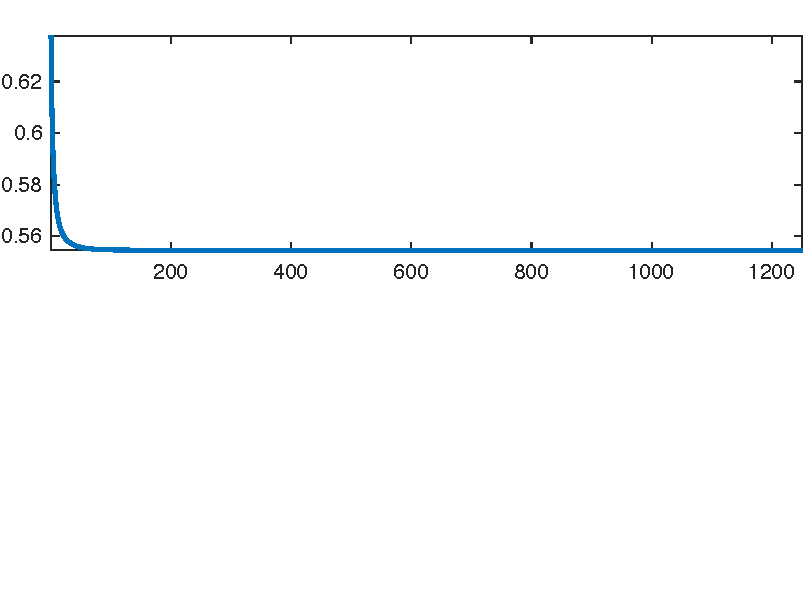
\includegraphics[width=.45\linewidth]{ml/sgd/error-bgd-1} &
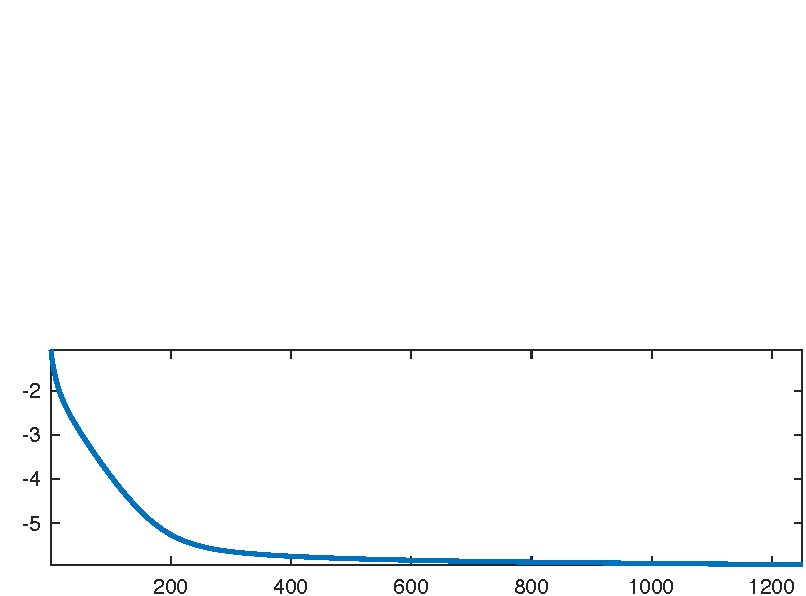
\includegraphics[width=.45\linewidth]{ml/sgd/error-bgd-2} \\
$f(x_k)$ & $\log_{10}(f(x_k)-f(x^\star))$ 
\end{tabular}
\caption{\label{fig-bgd}
Evolution of the error of the BGD for logistic classification.
}
\end{figure}



%%%%%%%%%%%%%%%%%%%%%%%%%%%%%%%%%%%%%%%%%%%%%%%%%%%%%%%%
\subsection{Stochastic Gradient Descent (SGD)}

\wrapf{ml/sgd/unbiased-grad}{Unbiased gradient estimate}
For very large $n$, computing the full gradient $\nabla f$ as in~\eqref{eq-full-grad} is prohibitive.  
%
The idea of SGD is to trade this exact full gradient by an inexact proxy using a single functional $f_{i}$ where $i$ is drawn uniformly at random. The main idea that makes this work is that this sampling scheme provides an unbiased estimate of the gradient, in the sense that
\eql{\label{eq-unbiased-grad}
	\EE_{\ip}{ \nabla f_{\ip}(x) } = \nabla f(x)
}
where $\ip$ is a random variable distributed uniformly in $\{1,\ldots,n\}$.

\wrapf{ml/sgd/sgd-schematic}{Schematic view of SGD iterates}
Starting from some $x_0$,the iterations of stochastic gradient descent (SGD) read
\eq{
	x_{k+1} = x_k - \tau_k \nabla f_{i(k)}(x_k)
}
where, for each iteration index $k$, $i(k)$
is drawn uniformly at random in $\{1,\ldots,n\}$. 
%
It is important that the iterates $x_{k+1}$ are thus random vectors, and the theoretical analysis of the method thus studies wether this sequence of random vectors converges (in expectation or in probability for instance) toward a deterministic vector (minimizing $f$), and at which speed. 

Note that each step of a batch gradient descent has complexity $O(np)$,
while a step of SGD only has complexity $O(p)$. SGD is thus
advantageous when $n$ is very large, and one cannot afford to do
several passes through the data. In some situation, SGD can provide
accurate results even with $k \ll n$, exploiting redundancy between
the samples.

A crucial question is the choice of step size schedule $\tau_k$. It
must tends to 0 in order to cancel the noise induced on the gradient by
the stochastic sampling. But it should not go too fast to zero in order
for the method to keep converging. 


A typical schedule that ensures both properties is to have asymptotically $\tau_k \sim k^{-1}$ for
$k\rightarrow +\infty$. We thus propose to use 
\eql{\label{eq-stepsize-sgd}
	\tau_k \eqdef \frac{\tau_0}{1 + k/k_0}
}
where $k_0$ indicates roughly the number of iterations serving as a
``warmup'' phase.

Figure~\ref{fig-sgd-traject} shows a simple 1-D example to minimize $f_1(x)+f_2(x)$ for $x \in \RR$ and $f_1(x)=(x-1)^2$ and $f_2(x)=(x+1)^2$. One can see how the density of the distribution of $x_k$ progressively clusters around the minimizer $x^\star=0$. Here the distribution of $x_0$ is uniform on $[-1/2,1/2]$.

\begin{figure}
\centering
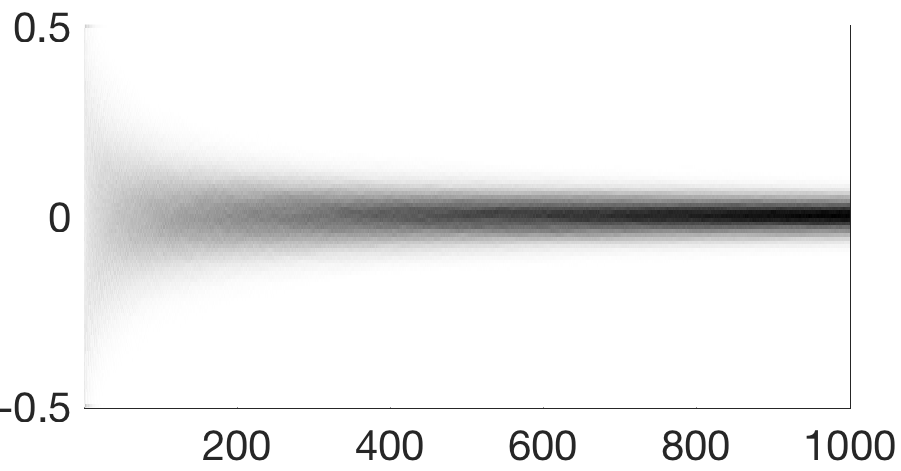
\includegraphics[width=.49\linewidth]{ml/sgd/sgd-histo} 
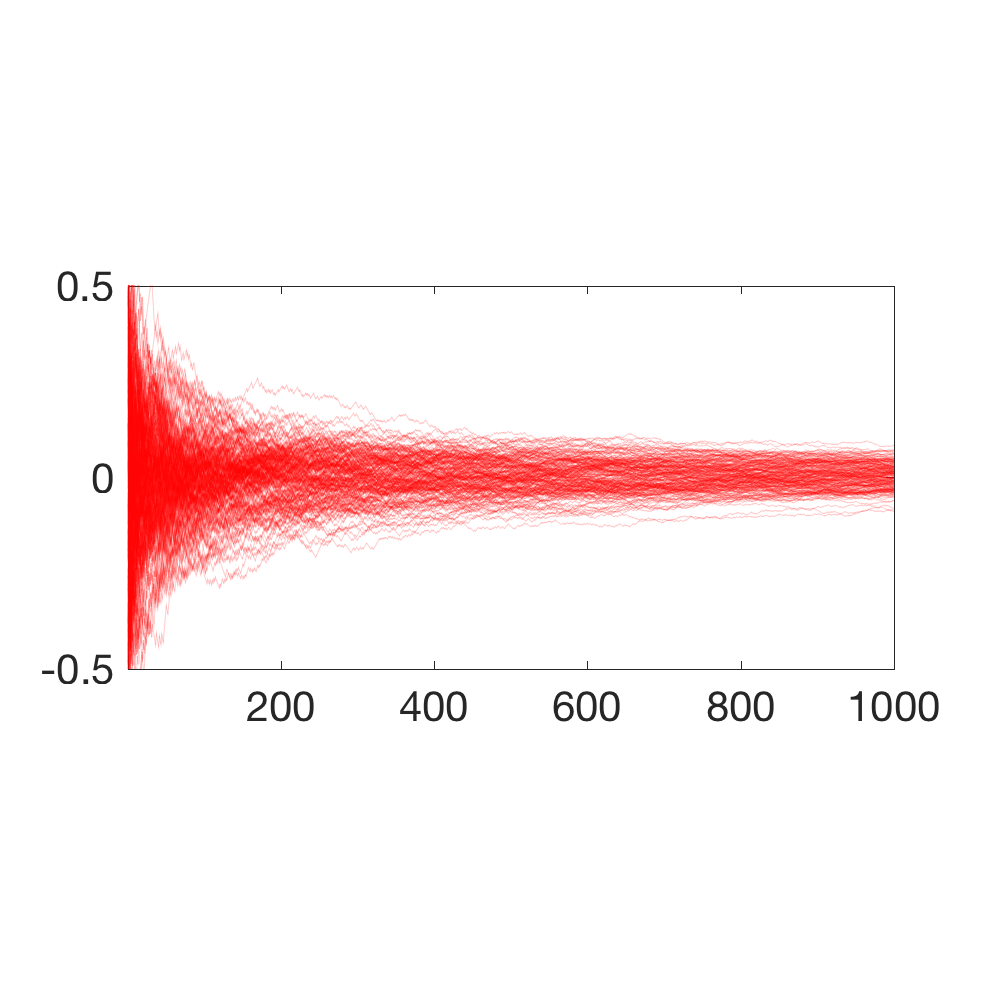
\includegraphics[width=.49\linewidth]{ml/sgd/sgd-trajectory}
\caption{\label{fig-sgd-traject}
Display of a large number of trajectories $k \mapsto x_k \in \RR$ generated by several runs of SGD. On the top row, each curve is a trajectory, and the bottom row displays the corresponding density.
}
\end{figure}

The following theorem shows the convergence in expectation with a $1/\sqrt{k}$ rate on the objective.

\begin{thm}\label{thm-conv-sgd}
We assume $f$ is $\mu$-strongly convex as defined in~\eqref{eq-strong-conv} (i.e. $\Id_{p}  \preceq \partial^2  f(x)$ if $f$ is $\Cc^2$), and is such that $\norm{\nabla f_i(x)}^2 \leq C^2$. 
For the step size choice $\tau_k = \frac{1}{\mu (k+1)}$, one has
\eql{\label{eq-rate-sgd}
	\EE( \norm{x_k-x^\star}^2 ) \leq \frac{ R }{k+1}
	\qwhereq
	 R = \max( \norm{x_0 - x^\star}, C^2/\mu^2 ), 
}
where $\EE$ indicates an expectation with respect to the i.i.d.
sampling performed at each iteration.
\end{thm}

\begin{proof}
	By strong convexity, one has
	\begin{align*}
		f(x^\star) - f(x_k) &\geq \dotp{ \nabla f(x_k) }{ x^\star-x_k } + \frac{\mu}{2}\norm{x_k-x^\star}^2 \\
		f(x_k) - f(x^\star) &\geq \dotp{ \nabla f(x^\star) }{ x_k - x^\star } + \frac{\mu}{2}\norm{x_k-x^\star}^2.
	\end{align*}
	Summing these two inequalities and using $\nabla f(x^\star)=0$ leads to
	\eql{\label{eq-sgd-proof-1}
		\dotp{ \nabla f(x_k) - \nabla f(x^\star) }{ x_k - x^\star }
		=
		\dotp{ \nabla f(x_k)  }{ x_k - x^\star }
		\geq \mu \norm{x_k-x^\star}^2.
	}
	Considering only the expectation with respect to the ransom sample of $i(k) \sim \ip_k$, one has
	\begin{align*}
		\EE_{\ip_k}( \norm{x_{k+1}-x^\star}^2 )
		&= 
		\EE_{\ip_k}( \norm{x_k - \tau_k \nabla f_{\ip_k}(x_k) -x^\star}^2 ) \\
		&= 
		\norm{x_k - x^\star}^2 + 2\tau_k \dotp{ \EE_{\ip_k}(\nabla f_{\ip_k}(x_k)) }{ x^\star - x_k  } + 
			\tau_k^2  \EE_{\ip_k}( \norm{\nabla f_{\ip_k}(x_k)}^2 ) \\
		&\leq
		\norm{x_k - x^\star}^2 + 2\tau_k \dotp{ \nabla f(x_k)) }{ x^\star - x_k  } + \tau_k^2 C^2 \\
	\end{align*}
	where we used the fact~\eqref{eq-unbiased-grad} that the gradient is unbiased. 
	%
	Taking now the full expectation with respect to all the other previous iterates, and using~\eqref{eq-sgd-proof-1} one obtains
	\eql{\label{eq-sgd-proof-2}
		\EE( \norm{x_{k+1}-x^\star}^2 ) \leq \EE( \norm{x_k - x^\star}^2 ) - 2 \mu \tau_k \EE( \norm{x_k - x^\star}^2 ) + \tau_k^2 C^2
		= (1-2 \mu \tau_k)  \EE( \norm{x_k - x^\star}^2 ) + \tau_k^2 C^2.
	}
	We show by recursion that the bound~\eqref{eq-rate-sgd} holds. We denote $\epsilon_k \eqdef \EE( \norm{x_k-x^\star}^2 )$.
	%
	Indeed, for $k=0$, this it is true that 
	\eq{
		\epsilon_0 \leq \frac{ \max( \norm{x_0 - x^\star}, C^2/\mu^2 ) }{1} = \frac{R}{1}.
	}
	We now assume that $\epsilon_k \leq \frac{R}{k+1}$. Using~\eqref{eq-sgd-proof-2} in the case of $\tau_k = \frac{1}{\mu (k+1)}$, one has, denoting $m=k+1$
	\begin{align*}
		\epsilon_{k+1} &\leq (1-2 \mu \tau_k) \epsilon_k + \tau_k^2 C^2 = 
			\pa{1-\frac{2}{m}} \epsilon_k + \frac{C^2}{(\mu m)^2}  \\  
			&\leq
			\pa{1-\frac{2}{m}} \frac{R}{m} + \frac{R}{m^2}  = 
			\pa{ \frac{1}{m}-\frac{1}{m^2} } R
			= 
			\frac{m-1}{m^2} R
			= 
			\frac{m^2-1}{m^2}\frac{1}{m+1} R
			\leq
			\frac{R}{m+1}
	\end{align*}
\end{proof}

A weakness of SGD (as well as the SGA scheme studied next) is that it only weakly benefit from strong convexity of $f$. This is in sharp contrast with BGD, which enjoy a fast linear rate for strongly convex functionals, see Theorem~\ref{thm-gradsec-non-strong-conv}.

Figure~\ref{fig-sgd} displays the evolution of the energy $f(x_k)$. 
It overlays on top (black dashed curve) the convergence of the batch gradient descent, with a careful scaling of the 
number of iteration to account for the fact that the complexity of a batch iteration is $n$ times larger. 


\begin{figure}
\centering
\begin{tabular}{cc}
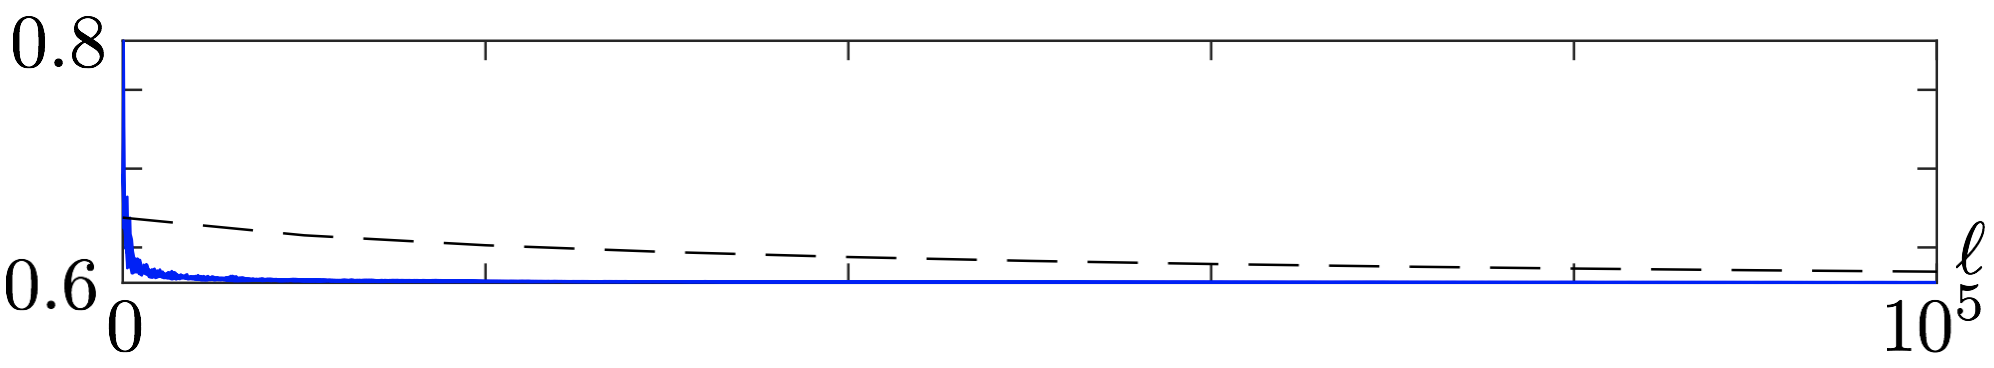
\includegraphics[width=.45\linewidth]{ml/sgd/error-sgd-1} &
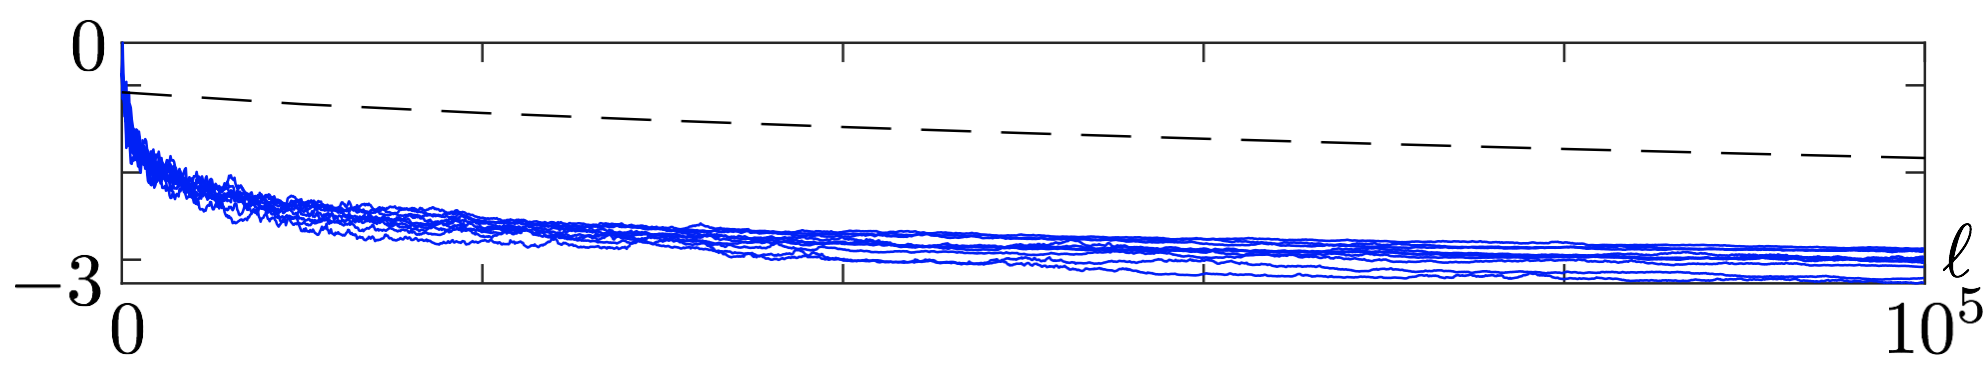
\includegraphics[width=.45\linewidth]{ml/sgd/error-sgd-2} \\
$f(x_k)$ & $\log_{10}(f(x_k)-f(x^\star))$ 
\end{tabular}
\caption{\label{fig-sgd}
Evolution of the error of the SGD for logistic classification (dashed line shows BGD).
}
\end{figure}




%%%%%%%%%%%%%%%%%%%%%%%%%%%%%%%%%%%%%%%%%%%%%%%%%%%%%%%%
\subsection{Stochastic Gradient Descent with Averaging (SGA)}
\label{sec-sga}

Stochastic gradient descent is slow because of the fast decay of
$\tau_k$ toward zero.
%
To improve somehow the convergence speed, it is possible to average the past
iterate, i.e. run a ``classical" SGD on auxiliary variables $( \tilde x_k)_k$
\eq{
	 \iit{\tilde x} = \tilde x_k - \tau_k \nabla f_{i(k)}(\tilde x_k)
}
and output as estimated weight vector the Cesaro average
\eq{
	x_k \eqdef \frac{1}{k} \sum_{\ell=1}^k \tilde x_{\ell}.
}
This defines the Stochastic Gradient Descent with Averaging (SGA)
algorithm.

Note that it is possible to avoid explicitly storing all the iterates by simply
updating a running average as follow
\eq{
	x_{k+1} = \frac{1}{k} \tilde x_k +  \frac{k-1}{k} x_k. 
}


In this case, a typical choice of decay is rather of the form 
\eq{
	\tau_k \eqdef \frac{\tau_0}{1 + \sqrt{k/k_0}}.
}
Notice that the step size now goes much slower to 0, at rate $k^{-1/2}$.


Typically, because the averaging stabilizes the iterates, the choice of
$(k_0,\tau_0)$ is less important than for SGD. 

% <https://arxiv.org/pdf/1303.6149.pdf 

Bach proves that for logistic classification, 
it leads to a faster convergence (the constant involved are
smaller) than SGD, since 
on contrast to SGD, SGA is adaptive to the local strong convexity of $E$.



%%%%%%%%%%%%%%%%%%%%%%%%%%%%%%%%%%%%%%%%%%%%%%%%%%%%%%%%
\subsection{Stochastic Averaged Gradient Descent (SAG)}

% https://arxiv.org/pdf/1309.2388
For problem size $n$ where the dataset (of size $n \times p$) can
fully fit into memory, it is possible to further improve the SGA method
by bookkeeping the previous gradients. This gives rise to the 
Stochastic Averaged Gradient Descent (SAG) algorithm.

We store all the previously computed gradients in $(G^i)_{i=1}^n$,
which necessitates $O(n \times p)$ memory. 
The iterates are defined by using a proxy $g$ for the batch gradient,
which is progressively enhanced during the iterates.

The algorithm reads
\eq{
	x_{k+1} = x_k - \tau g
	\qwhereq
	\choice{
	h \leftarrow \nabla f_{i(k)}(\tilde x_k), \\
	g  \leftarrow g - G^{i(k)} + h,   \\
	G^{i(k)} \leftarrow h.
	}
}
Note that in contrast to SGD and SGA, this method uses a fixed step
size $\tau$. Similarly to the BGD, in order to ensure convergence, 
the step size $\tau$ should be of the order of $1/L$
where $L$ is the Lipschitz constant of $f$.

This algorithm improves over SGA and SGD
since it has a convergence rate of $O(1/k)$ as does BGD. 
Furthermore, in the presence of strong convexity (for instance when $X$ is
injective for logistic classification), it has a linear convergence rate, 
i.e. 
 \eq{
	\EE( f(x_k) ) - f(x^\star) = O\pa{ \rho^k },
}
for some $0 < \rho < 1$. 

Note that this improvement over SGD and SGA is made possible only because
SAG explicitly uses the fact that $n$ is finite (while SGD and SGA can
be extended to infinite $n$ and more general minimization of
expectations~\eqref{eq-min-int}).

Figure~\ref{fig-compariso-sgd} shows a comparison of SGD, SGA and SAG.

\begin{figure}
\centering
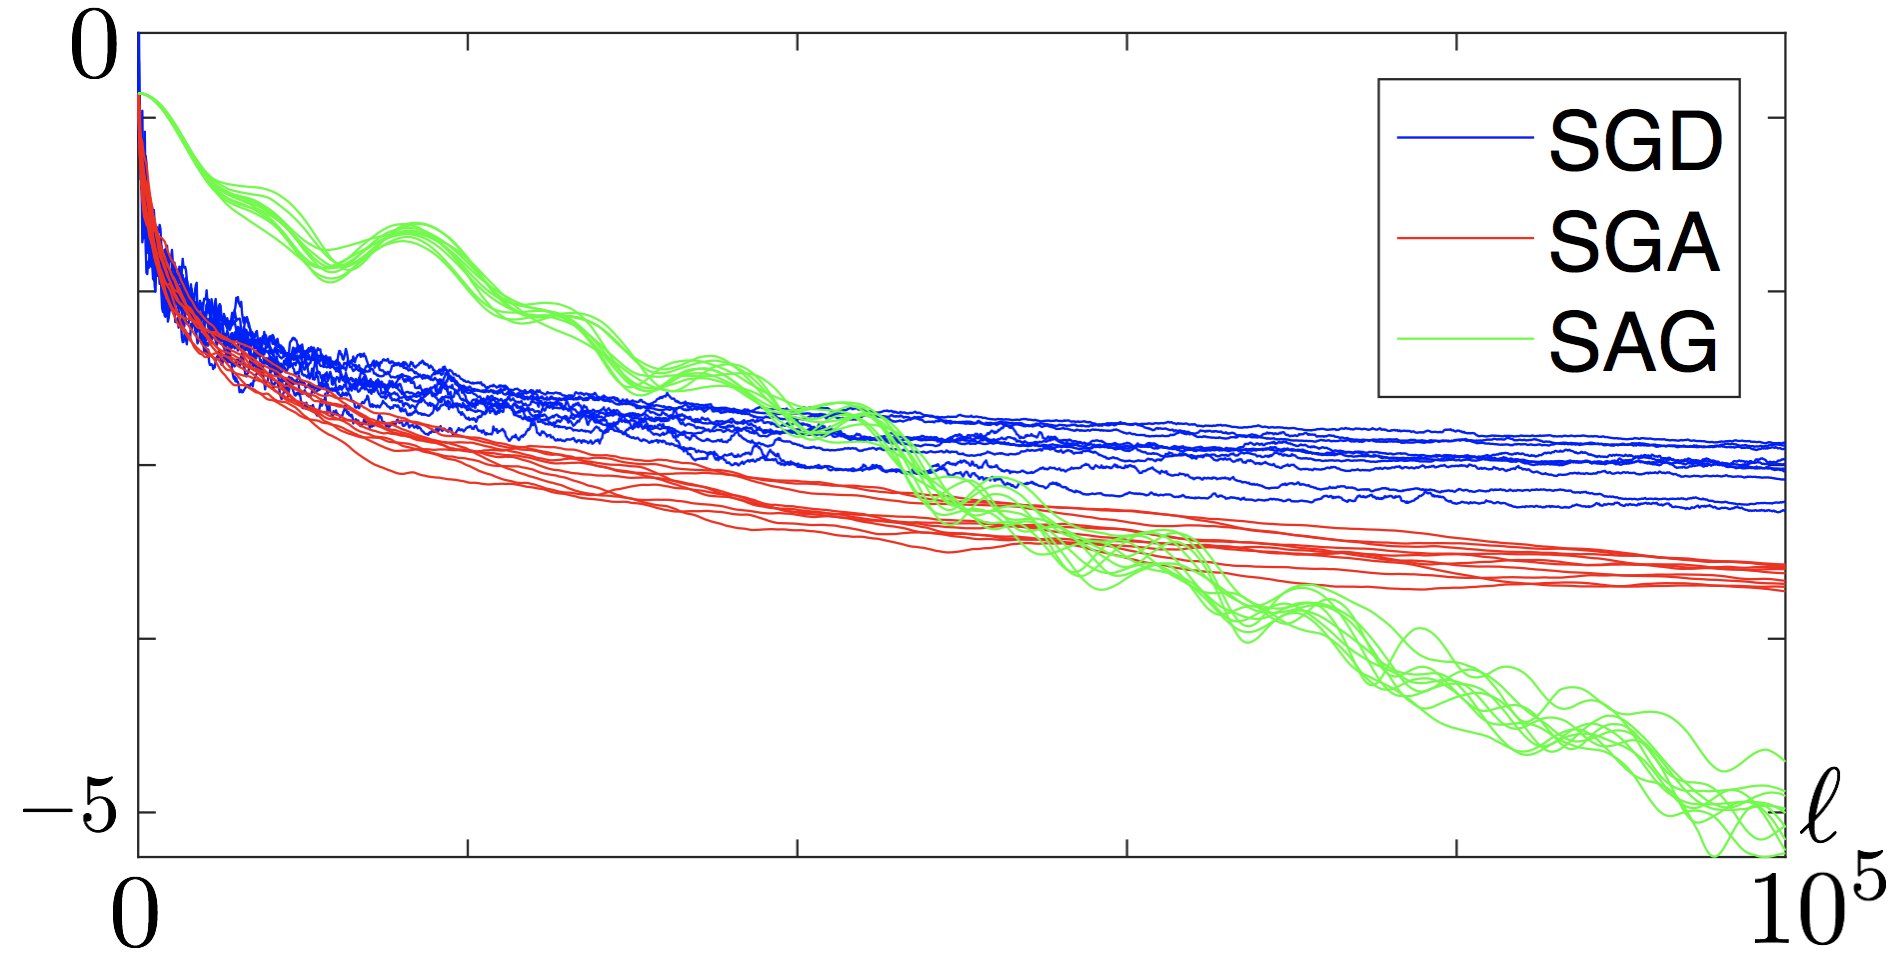
\includegraphics[width=.5\linewidth]{ml/sgd/sg-comparison}
\caption{\label{fig-compariso-sgd}
Evolution of $\log_{10}(f(x_k)-f(x^\star))$ for SGD, SGA and SAG.
}
\end{figure}




\input{../chapters/sec-mlp}

\section{Automatic Differentiation}
% !TEX root = ../auto-diff/AutoDiff.tex

%%% SECTION PART OF optim-smooth.tex



The main computational bottleneck of gradient descent methods (batch or stochastic) is the computation of gradients $\nabla f(x)$. For simple functionals, such as those encountered in ERM for linear models, and also for MLP with a single hidden layer, it is possible to compute these gradients in closed form, and that the main computational burden is the evaluation of matrix-vector products. For more complicated functionals (such as those involving deep networks), computing the formula for the gradient quickly becomes cumbersome. Even worse: computing these gradients using the usual chain rule formula is sub-optimal. We presents methods to compute recursively in an optimal manner these gradients. The purpose of this approach is to automatize this computational step.  

%%%%%%%%%%%%%%%%%%%%%%%%%%%%%%%%%%%%%%%%%%%%%%%%%%%%%%%%%%%%%%%%%%%%%%%%
\subsection{Finite Differences and Symbolic Calculus}

We consider $f : \RR^p \rightarrow \RR$ and want to derive a method to evaluate $\nabla f : \RR^p \mapsto \RR^p$. Approximating this vector field using finite differences, i.e. introducing $\epsilon>0$ small enough and computing 
\eq{
 	\frac{1}{\epsilon}(f(x+\epsilon \de_1)-f(x), \ldots,f(x+\epsilon \de_p)-f(x))^\top	\approx \nabla f(x)
}
requires $p+1$ evaluations of $f$, where we denoted $\de_k=(0,\ldots,0,1,0,\ldots,0)$ where the $1$ is at index $k$. 
%
For a large $p$, this is prohibitive. The method we  describe in this section (the so-called reverse mode automatic differentiation) has in most cases a cost proportional to a single evaluation of $f$. 
%
This type of method is similar to symbolic calculus in the sense that it provides (up to machine precision) exact gradient computation. But symbolic calculus does not takes into account the underlying algorithm which compute the function, while automatic differentiation factorizes the computation of the derivative according to an efficient algorithm.


%%%%%%%%%%%%%%%%%%%%%%%%%%%%%%%%%%%%%%%%%%%%%%%%%%%%%%%%%%%%%%%%%%%%%%%%
\subsection{Computational Graphs}

We consider a generic function $f(x)$ where $x=(x_1,\ldots,x_s)$ are the input variables. We assume that $f$ is implemented in an algorithm, with intermediate variable $(x_{s+1},\ldots,x_t)$ where $t$ is the total number of variables. The output is $x_t$, and we thus denote $x_t=f(x)$ this function. We denote $x_k \in \RR^{n_k}$ the dimensionality of the variables. The goal is to compute the derivatives $\pd{f(x)}{x_k} \in \RR^{n_t \times n_k}$ for $k=1,\ldots,s$. For the sake of simplicity, one can assume in what follows that $n_k=1$ so that all the involved quantities are scalar (but if this is not the case, beware that the order of multiplication of the matrices of course matters).

\begin{figure}
\centering
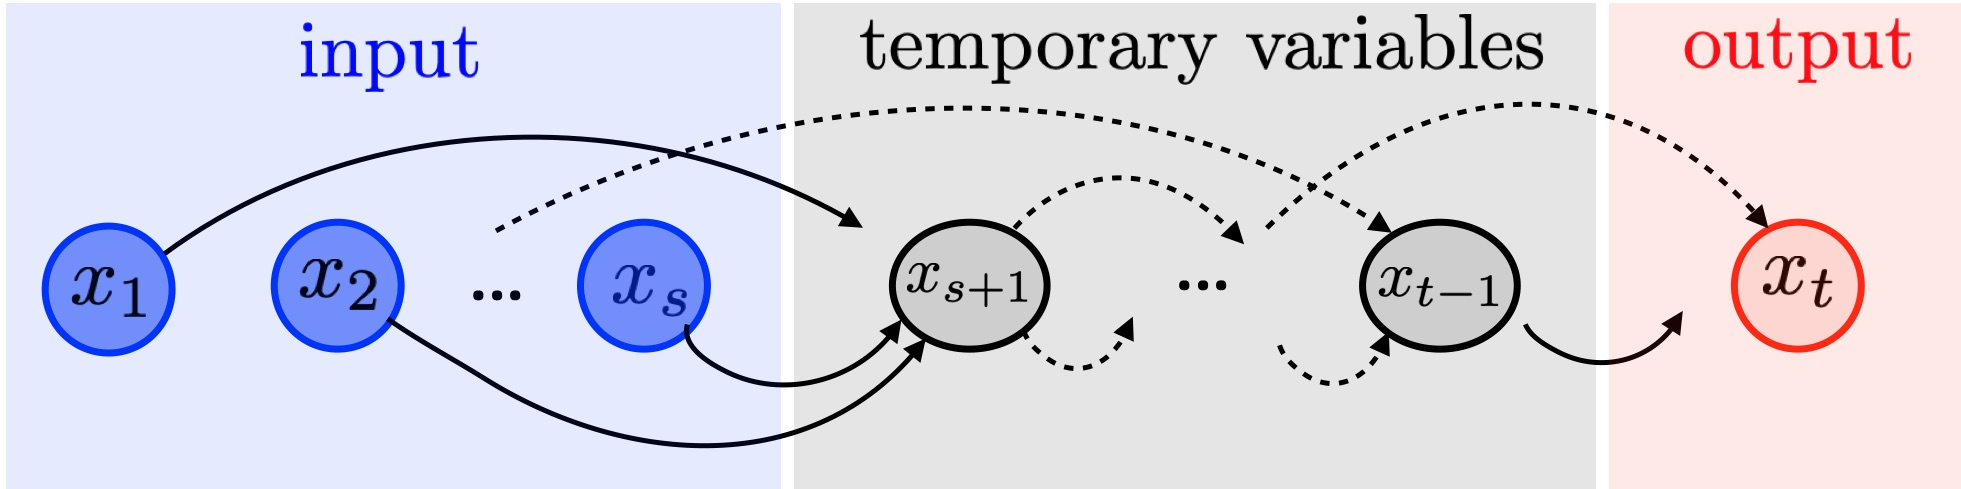
\includegraphics[width=.7\linewidth]{auto-diff/comp-graph}
\caption{\label{fig-compgraph}
A computational graph.
}
\end{figure}

A numerical algorithm can be represented as a succession of functions of the form
\eq{
	\foralls k=s+1,\ldots,t, \quad x_k = f_k( x_1,\ldots,x_{k-1} )
}
where $f_k$ is a function which only depends on the previous variables, see Fig.~\ref{fig-compgraph}. One can represent this algorithm using a directed acyclic graph (DAG), linking the variables involved in $f_k$ to $x_k$. The node of this graph are thus conveniently ordered by their indexing, and the directed edges only link a variable to another one with a strictly larger index.
%
The evaluation of $f(x)$ thus corresponds to a forward traversal of this graph. 
% 
Note that the goal of automatic differentiation is not to define an efficient computational graph, it is up to the user to provide this graph. Computing an efficient graph associated to a mathematical formula is a complicated combinatorial problem, which still has to be solved by the user. Automatic differentiation thus leverage the availability of an efficient graph to provide an efficient algorithm to evaluate derivatives. 



%%%%%%%%%%%%%%%%%%%%%%%%%%%%%%%%%%%%%%%%%%%%%%%%%%%%%%%%%%%%%%%%%%%%%%%%
\subsection{Forward Mode of Automatic Differentiation}

The forward mode correspond to the usual way of computing differentials. It compute the derivative $\pd{x_k}{x_1}$ of all variables $x_k$ with respect to $x_1$. One then needs to repeat this method $p$ times to compute all the derivative with respect to $x_1,x_2,\ldots,x_p$ (we only write thing for the first variable, the method being of course the same with respect to the other ones).

\newcommand{\bk}[1]{\left[#1\right]}
\newcommand{\pdb}[2]{\bk{\pd{#1}{#2}}}

\begin{figure}
\centering
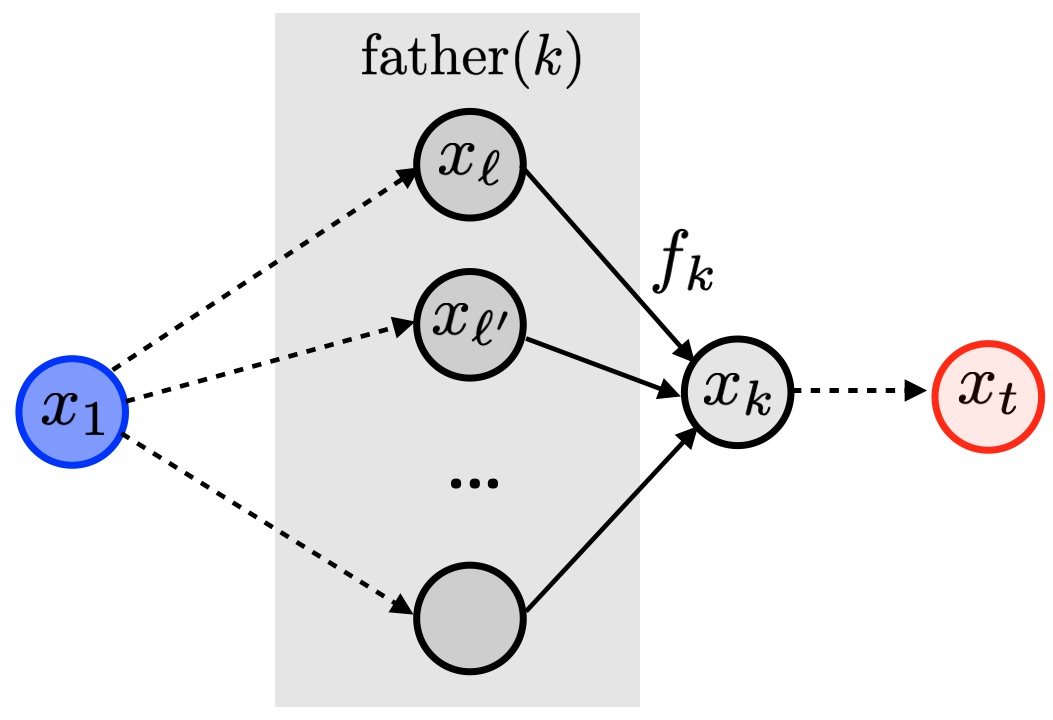
\includegraphics[width=.4\linewidth]{auto-diff/forward-mode}
\quad
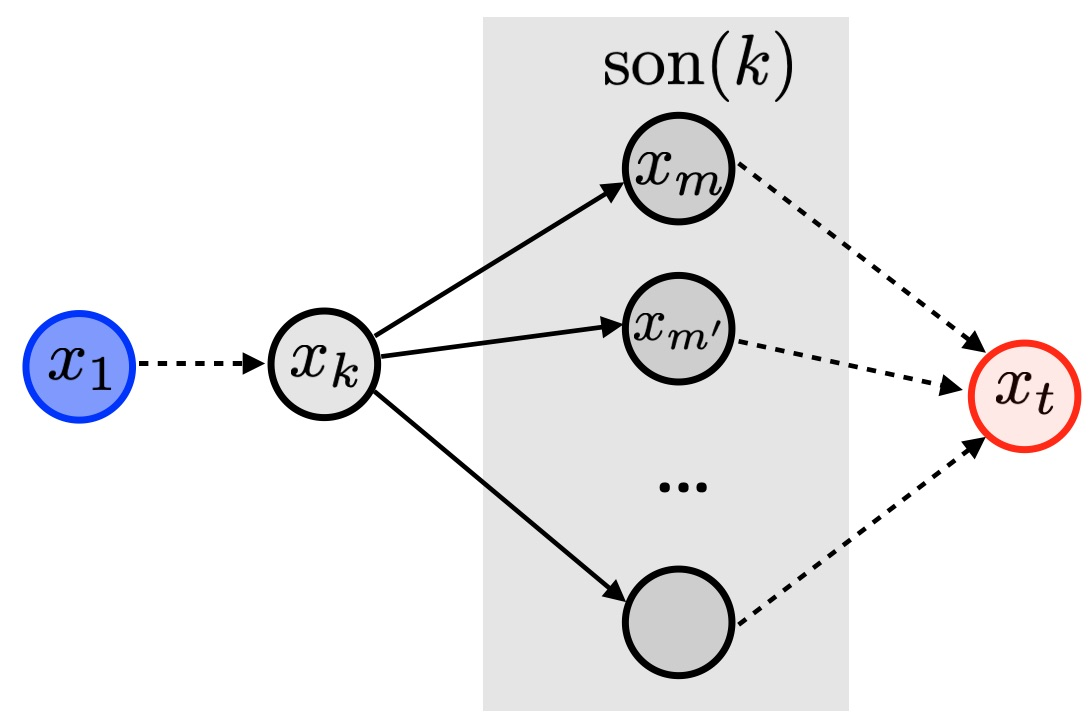
\includegraphics[width=.4\linewidth]{auto-diff/backward-mode}
\caption{\label{fig-forward-backward}
Relation between the variable for the forward (left) and backward (right) modes.
}
\end{figure}

The method initialize the derivative of the input nodes 
\eq{
	\pd{x_1}{x_1} = \Id_{n_1 \times n_1}, \quad 
	\pd{x_2}{x_1} = 0_{n_2 \times n_1}, \ldots, \quad
	\pd{x_s}{x_1} = 0_{n_s \times n_1}, 
}
(and thus 1 and 0's for scalar variables), and then iteratively make use of the following recursion formula
\eq{
	\foralls k=s+1,\ldots,t, \quad
	\pd{x_k}{x_1} 
	= \sum_{\ell \in \text{parent}(k)} \bk{\pd{x_k}{x_\ell}} \times \pd{x_\ell}{x_1}
	= \sum_{\ell \in \text{parent}(k)} \pd{f_k}{x_\ell}(x_1,\ldots,x_{k-1}) \times \pd{x_\ell}{x_1}.
}
The notation ``$\text{parent}(k)$'' denotes the nodes $\ell<k$ of the graph that are connected to $k$, see Figure~\ref{fig-forward-backward}, left. 
%
Here the quantities being computed (i.e. stored in computer variables) are the derivatives $\pd{x_\ell}{x_1}$, and $\times$ denotes in full generality matrix-matrix multiplications.
%
We have put in $[\ldots]$ an informal notation, since here $\pd{x_k}{x_\ell}$ should be interpreted not as a numerical variable but needs to be interpreted as derivative of the function $f_k$, which can be evaluated on the fly (we assume that the derivative of the function involved are accessible in closed form).  

Assuming all the involved functions $\pd{f_k}{x_k}$ have the same complexity (which is likely to be the case if all the $n_k$ are for instance scalar or have the same dimension), and that the number of parent node is bounded, one sees that the complexity of this scheme is $p$ times the complexity of the evaluation of $f$ (since this needs to be repeated $p$ times for $\pd{}{x_1},\ldots,\pd{}{x_p}$). For a large $p$, this is prohibitive. 



%%%
\paragraph{Simple example.}


We consider the fonction 
\eql{\label{eq-simple-func-autodiff}
 	f(x,y) = y\log(x)+\sqrt{y\log(x)}
} 
whose computational graph is displayed on Figure~\ref{fig-dag-example-simple}. The iterations of the forward mode to compute the derivative with respect to $x$ read
\begin{align*}
		\pd{x}{x} &= 1,  \quad \pd{y}{x} = 0 \\
		\pd{a}{x} &= \bk{\pd{a}{x}} \pd{x}{x} = \frac{1}{x} \pd{x}{x} &
			\{x \mapsto a = \log(x)\}\\
		\pd{b}{x} &= \bk{\pd{b}{a}} \pd{a}{x}  + \bk{\pd{b}{y}} \pd{y}{x}  = y \pd{a}{x} + 0 &
			\{(y,a) \mapsto b=ya\}\\
		\pd{c}{x} &= \bk{\pd{c}{b}} \pd{b}{x}  = \frac{1}{2\sqrt{b}} \pd{b}{x}&
			\{b \mapsto c=\sqrt{b}\} \\
		\pd{f}{x} &= \bk{\pd{f}{b}} \pd{b}{x} + \bk{\pd{f}{c}} \pd{c}{x}  = 1\pd{b}{x} + 1\pd{c}{x}&
			\{(b,c) \mapsto f=b+c\}
\end{align*}
One needs to run another forward pass to compute the derivative with respect to $y$
\begin{align*}
		\pd{x}{y} &= 0,  \quad \pd{y}{y} = 1 \\
		\pd{a}{y} &= \bk{\pd{a}{x}} \pd{x}{y} = 0 &
			\{x \mapsto a = \log(x)\}\\
		\pd{b}{y} &= \bk{\pd{b}{a}} \pd{a}{y}  + \bk{\pd{b}{y}} \pd{y}{y}  = 0 + a \pd{y}{y}  &
			\{(y,a) \mapsto b=ya\}\\
		\pd{c}{y} &= \bk{\pd{c}{b}} \pd{b}{y}  = \frac{1}{2\sqrt{b}} \pd{b}{y}&
			\{b \mapsto c=\sqrt{b}\} \\
		\pd{f}{y} &= \bk{\pd{f}{b}} \pd{b}{y} + \bk{\pd{f}{c}} \pd{c}{y}  = 1\pd{b}{y} + 1\pd{c}{y}&
			\{(b,c) \mapsto f=b+c\}
\end{align*}



\begin{figure}
\centering
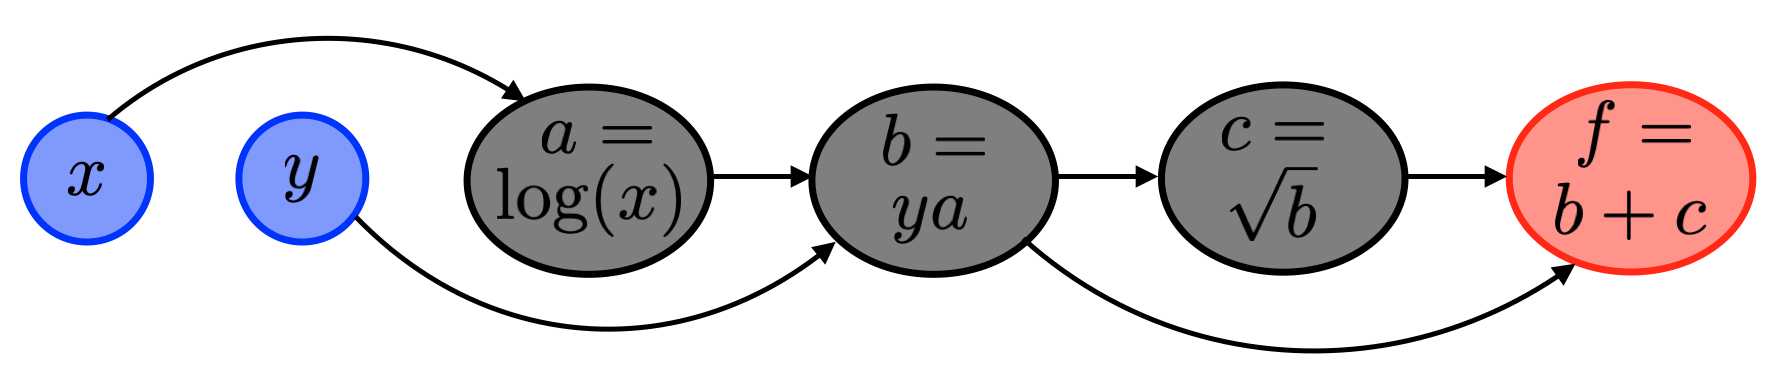
\includegraphics[width=.6\linewidth]{auto-diff/example-simple}
\caption{\label{fig-dag-example-simple}
Example of a simple computational graph.
}
\end{figure}

\if 0
%%%
\paragraph{Simple example.}

We consider the fonction 
\eql{\label{eq-simple-func-autodiff}
 	f(x) = \log(x)+\sqrt{\log(x)}
} 
whose computational graph is displayed on Figure~\ref{fig-dag-example-simple}. The iterations of the forward mode read
\begin{align*}
		\pd{x}{x} &= 1 \\
		\pd{y}{x} &= \bk{\pd{y}{x}} \pd{x}{x} = \frac{1}{x} \pd{x}{x} &
			\{x \mapsto y = \log(x)\}\\
		\pd{z}{x} &= \bk{\pd{z}{y}} \pd{y}{x} = \frac{1}{2\sqrt{y}} \pd{y}{x} &
			\{y \mapsto z=\sqrt{y}\}\\
		\pd{f}{x} &= \bk{\pd{f}{z}} \pd{z}{x} + \bk{\pd{f}{y}} \pd{y}{x} = 1 \pd{z}{x} + 1 \pd{y}{x}&
			\{(x,z) \mapsto f=x+z\}
\end{align*}



\begin{figure}
\centering
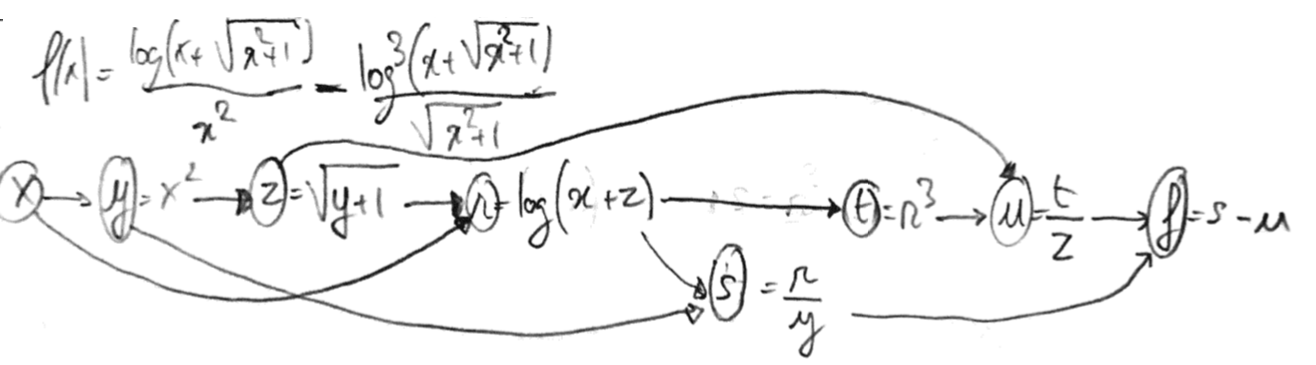
\includegraphics[width=.6\linewidth]{auto-diff/example-complex}
\caption{\label{fig-dag-example-complex}
Example of a more complex computational graph.
}
\end{figure}

%%%
\paragraph{More complex example.}

We now consider the fonction 
\eql{\label{eq-cpx-func-autodiff}
	f(x) = \frac{\log(x+\sqrt{x^2+1})}{x^2} - \frac{\log^3(x+\sqrt{x^2+1})}{\sqrt{x^2+1}}
}
whose computational graph is displayed on Figure~\ref{fig-dag-example-complex}. The iterations of the forward mode read
\begin{align*}
		\pd{x}{x} &= 1 \\
		\pd{y}{x} &= \pdb{y}{x} \pd{x}{x}  = 2 x \pd{x}{x}  &
			\{x \mapsto y = x^2\} \\
		\pd{z}{x} &= \pdb{z}{y} \pd{y}{x} = \frac{1}{2\sqrt{y+1}} \pd{y}{x} &
			\{y \mapsto z=\sqrt{y+1}\}\\
		\pd{r}{x} &= \pdb{r}{z} \pd{x}{x} + \pdb{r}{z} \pd{z}{x} = \frac{1}{x+r} \pd{x}{x} + \frac{1}{x+r} \pd{z}{x}&
			\{(x,z) \mapsto r=\log(x+z)\} \\
		\pd{s}{x} &= \pdb{s}{r} \pd{r}{x} + \pdb{s}{y}\pd{y}{x} = \frac{1}{y} \pd{r}{x} - \frac{r}{y^2}\pd{y}{x} &
			\{ (r,y) \mapsto s=\frac{r}{y}  \} \\
		\pd{t}{x} &= \pdb{t}{r} \pd{r}{x} = 3r^2 \pd{r}{x} &
			\{ r \mapsto t = r^3 \} \\
		\pd{u}{x} &= \pdb{u}{t} \pd{t}{x} + \pdb{u}{z}\pd{z}{x} = \frac{1}{z} \pd{t}{x} - \frac{t}{z^2} \pd{z}{x} &
			\{ (t,z) \mapsto u =  \frac{t}{z}  \} \\
		\pd{f}{x} &= \pdb{f}{s}\pd{s}{x} + \pdb{f}{u}\pd{u}{x} = 1 \pd{s}{x} - 1 \pd{u}{x} &
			\{ (s,u) \mapsto f = s-u \}
\end{align*}
\fi


%%%
\paragraph{Dual numbers.}

A convenient way to implement this forward pass is to make use of so called ``dual number'', which is an algebra over the real  where the number have the form $x + \epsilon x'$ where $\epsilon$ is a symbol obeying the rule that $\epsilon^2=0$. Here $(x,x') \in \RR^2$ and $x'$ is intended to store a derivative with respect to some input variable. These number thus obeys the following arithmetic operations
\eq{
	(x+\epsilon x')(y+\epsilon y') = xy + \epsilon (x y' + y x')
	\qandq
	\frac{1}{x+\epsilon x'} = \frac{1}{x}-\epsilon \frac{x'}{x^2}. 
}
If $f$ is a polynomial or a rational function, from these rules one has that 
\eq{
	f(x+\epsilon) = f(x) + \epsilon f'(x).
}
For a more general basic function $f$, one needs to overload it so that
\eq{
	f(x+\epsilon x') \eqdef f(x) + \epsilon f'(x) x'.
}
Using this definition, one has that 
\eq{
	(f \circ g)(x+\epsilon ) = f(g(x)) + \epsilon f'(g(x))g'(x)
}
which corresponds to the usual chain rule. More generally, if $f(x_1,\ldots,x_s)$ is a function implemented using these overloaded basic functions, one has  
\eq{
	f(x_1+\epsilon,x_2,\ldots,x_s) = f(x_1,\ldots,x_s) + \epsilon \pd{f}{x_1}(x_1,\ldots,x_s)
}
and this evaluation is equivalent to applying the forward mode of automatic differentiation to compute $\pd{f}{x_1}(x_1,\ldots,x_s)$ (and similarly for the other variables).


%%%%%%%%%%%%%%%%%%%%%%%%%%%%%%%%%%%%%%%%%%%%%%%%%%%%%%%%%%%%%%%%%%%%%%%%
\subsection{Reverse Mode of Automatic Differentiation}

Instead of evaluating the differentials $\pd{x_k}{x_1}$ which is problematic for a large $p$, the reverse mode evaluates the differentials  $\pd{x_t}{x_k}$, i.e. it computes the derivative of the output node with respect to the all the inner nodes. 



The method initialize the derivative of the final node
\eq{
	\pd{x_t}{x_t} = \Id_{n_t \times n_t}, 
}
and then iteratively makes use,  from the last node to the first, of the following recursion formula
\eq{
	\foralls k=t-1,t-2,\ldots,1, \quad
	\pd{x_t}{x_k} 
	= \sum_{m \in \text{son}(k)}  \pd{x_t}{x_m} \times \bk{\pd{x_m}{x_k}}
	= \sum_{m \in \text{son}(k)} \pd{x_t}{x_m} \times \pd{f_m(x_1,\ldots,x_m)}{x_k}.
}
%
The notation ``$\text{parent}(k)$'' denotes the nodes $\ell<k$ of the graph that are connected to $k$, see Figure~\ref{fig-forward-backward}, right. 

%%%
\paragraph{Back-propagation.}

In the special case where $x_t \in \RR$, then $\pd{x_t}{x_k} = [\nabla_{x_k} f(x)]^\top \in \RR^{1 \times n_k}$ and one can write the recursion on the gradient vector as follow 
\eq{
	\foralls k=t-1,t-2,\ldots,1, \quad
	\nabla_{x_k} f(x) 
	= \sum_{m \in \text{son}(k)} \pa{\pd{f_m(x_1,\ldots,x_m)}{x_k}}^\top \pa{
	 	\nabla_{x_m} f(x)
	}.
}
where $\pa{\pd{f_m(x_1,\ldots,x_m)}{x_k}}^\top \in \RR^{n_k \times n_m}$ is the adjoint of the Jacobian of $f_m$. This form of recursion using adjoint is often referred to as ``back-propagation'', and is the most frequent setting in applications to ML.

In general, when $n_t=1$, the backward is the optimal way to compute the gradient of a function. Its drawback is that it necessitate the pre-computation of all the intermediate variables $(x_k)_{k=p}^t$, which can be prohibitive in term of memory usage when $t$ is large. There exists check-pointing method to alleviate this issue, but it is out of the scope of this course.

%%%
\paragraph{Simple example.}

We consider once again the fonction $f(x)$ of~\eqref{eq-simple-func-autodiff}, the iterations of the reverse mode read
\begin{align*}
		\pd{f}{f} &= 1 &\\
		\pd{f}{c} &= \pd{f}{f} \pdb{f}{c} = \pd{f}{f} 1 &
			\{ c \mapsto f = b+c\}\\
		\pd{f}{b} &= \pd{f}{c} \pdb{c}{b} + \pd{f}{f} \pdb{f}{b} = \pd{f}{c} \frac{1}{2\sqrt{b}} + \pd{f}{f} 1 & 
			\{ b \mapsto c=\sqrt{b}, b \mapsto f=b+c\} \\
		\pd{f}{a} &= \pd{f}{b} \pdb{b}{a} = \pd{f}{b} y & 
			\{ a \mapsto b=y a\} \\
		\pd{f}{y} &= \pd{f}{b} \pdb{b}{y} = \pd{f}{b} a & 
			\{ y \mapsto b=ya\} \\
		\pd{f}{x} &= \pd{f}{a} \pdb{a}{x} = \pd{f}{a} \frac{1}{x} & 
			\{ x \mapsto a=\log(x)\}
\end{align*}
The advantage of the reverse mode is that a single traversal of the computational graph allows to compute both derivatives with respect to $x,y$, while the forward more necessitates two passes.

\if 0
%%%
\paragraph{More complex example.}

We consider once again the fonction $f(x)$ of~\eqref{eq-cpx-func-autodiff}, the iterations of the reverse mode read
\begin{align*}
		\pd{f}{f} &= 1 &\\
		\pd{f}{u} &= \pd{f}{f} \pdb{f}{u} 
			= \pd{f}{f} (-1) &
			\{u \mapsto f = s-u\}\\
		\pd{f}{t} &= \pd{f}{u} \pdb{u}{t} 
			= \pd{f}{u} \frac{1}{z}  & 
			\{ t \mapsto u= \sqrt{y}, y \frac{t}{z} \} \\
		\pd{f}{s} &= \pd{f}{f} \pdb{f}{s} = \pd{f}{f} 1 & 
			\{ s \mapsto f = s-u \} \\
		\pd{f}{r} &= \pd{f}{t} \pdb{t}{r} + \pd{f}{s} \pdb{s}{r} 
			= \pd{f}{t} 3r^2 + \pd{f}{s} \frac{1}{y} & 
			\{ r \mapsto s = \frac{r}{y}, r \mapsto  t=r^3\}  \\
		\pd{f}{z} &= \pd{f}{u} \pdb{u}{z} + \pd{f}{r} \pdb{r}{z} 
			= \pd{f}{u} \frac{-t}{z^2} + \pd{f}{r} \pdb{1}{x+z} &
			\{ z \mapsto u=\frac{t}{z}, z \mapsto r=\log(x+z)\} \\
		\pd{f}{y} &= \pd{f}{z}\pdb{z}{y} + \pd{f}{s}\pdb{s}{y}
			= \pd{f}{z} \frac{1}{2\sqrt{y+1}} + \pd{f}{s}\frac{-r}{y^2} &
			\{ y \mapsto z=\sqrt{y+1}, y \mapsto s = \frac{r}{y}\} \\
		\pd{f}{x} &= \pd{f}{y}\pdb{y}{x} + \pd{f}{r}\pdb{r}{x}
			= \pd{f}{y} 2x + \pd{f}{r} \frac{1}{x+z}  &
			\{x \mapsto y=x^2, x \mapsto r=\log(x+z)\}		
\end{align*}
\fi


%%%%%%%%%%%%%%%%%%%%%%%%%%%%%%%%%%%%%%%%%%%%%%%%%%%%%%%%%%%%%%%%%%%%%%%%
\subsection{Feed-forward Compositions}

The simplest computational graphs are purely feedforward, and corresponds to the computation of 
\eql{\label{eq-simple-lin-dag}
	f = f_{t} \circ f_{t-1} \circ \ldots \circ f_2 \circ f_1
}
for functions $f_k : \RR^{n_{k-1}} \rightarrow \RR^{n_{k}}$.

The forward function evaluation algorithm initializes $x_0=x \in \RR^{n_0}$ and then computes
\eq{
	\foralls k=1, \ldots, t, \quad x_{k} = f_k(x_{k-1})
}
where at the output, one retrieves $f(x) = x_t$.

Denoting $A_k \eqdef \partial f_k(x_{k-1}) \in \RR^{n_{k} \times n_{k-1}}$ the Jacobian, one has
\eq{
	\partial f(x) = A_{t} \times A_{t-1} \times \ldots A_2 \times A_1.
}
The forward (resp. backward) mode corresponds to the computation of the product of the Jacobian from right to left (resp. left to right) 
\begin{align*}
	\partial f(x) &= A_{t} \times \pa{  A_{t-1} \times \pa{ \ldots \times \pa{ A_3 \times \pa{ A_2 \times A_1 } } } }, \\
	\partial f(x) &= \pa{ \pa{ \pa{ \pa{ A_{t} \times A_{t-1} }  \times A_{t-2} } \times \ldots } \times A_2 } \times A_1.
\end{align*}


\begin{figure}
\centering
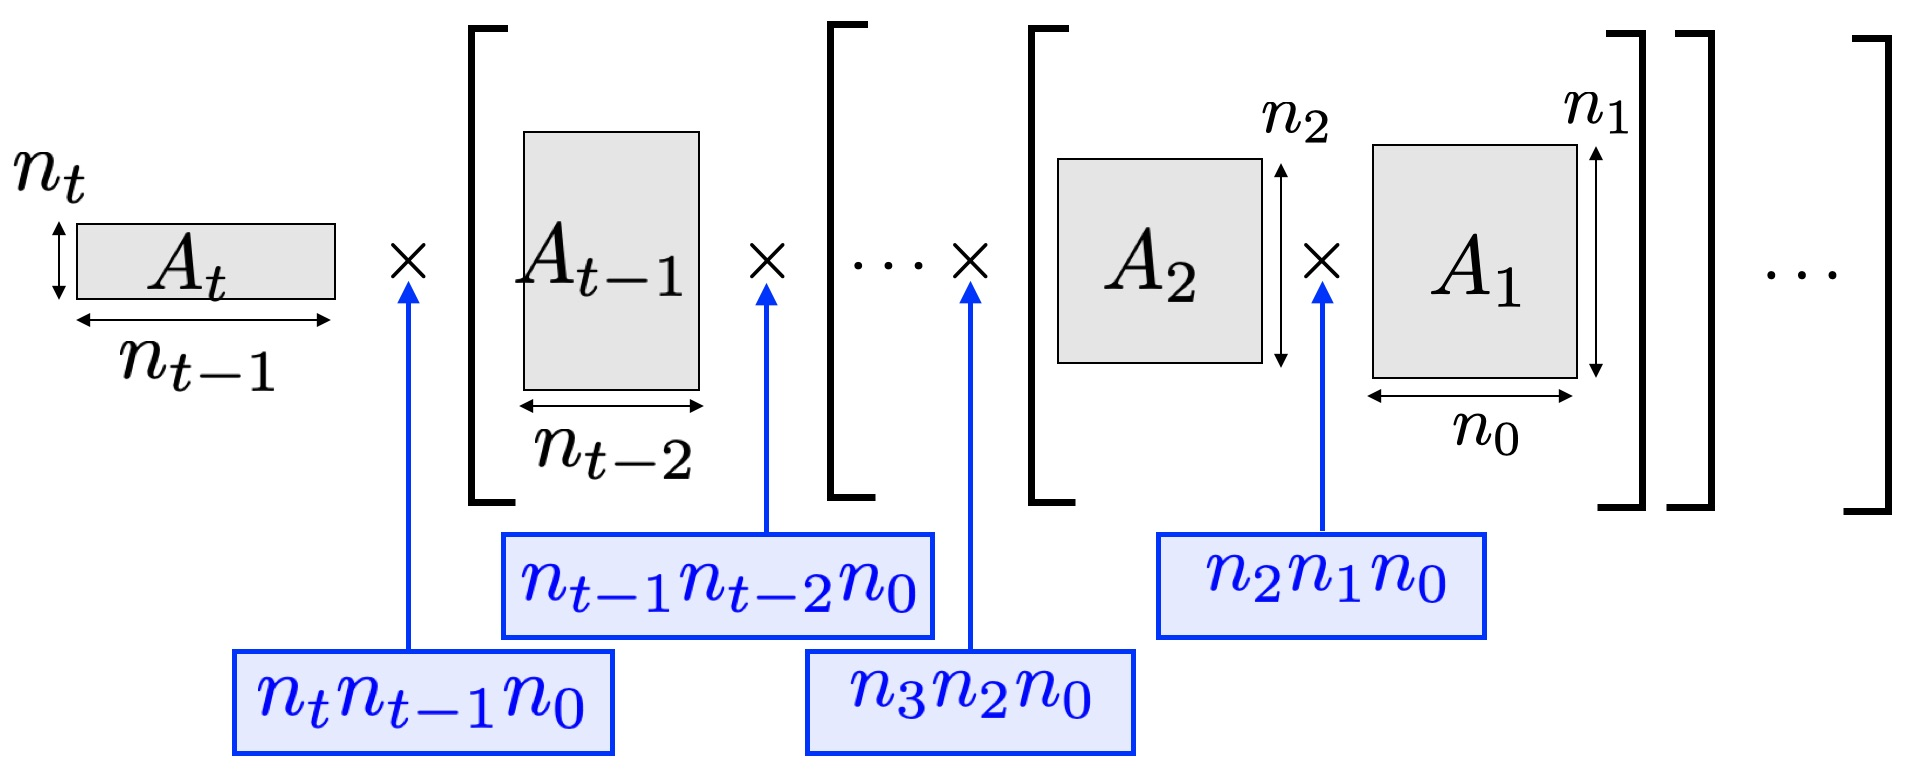
\includegraphics[width=.42\linewidth]{auto-diff/matrix-forward} 
\qquad
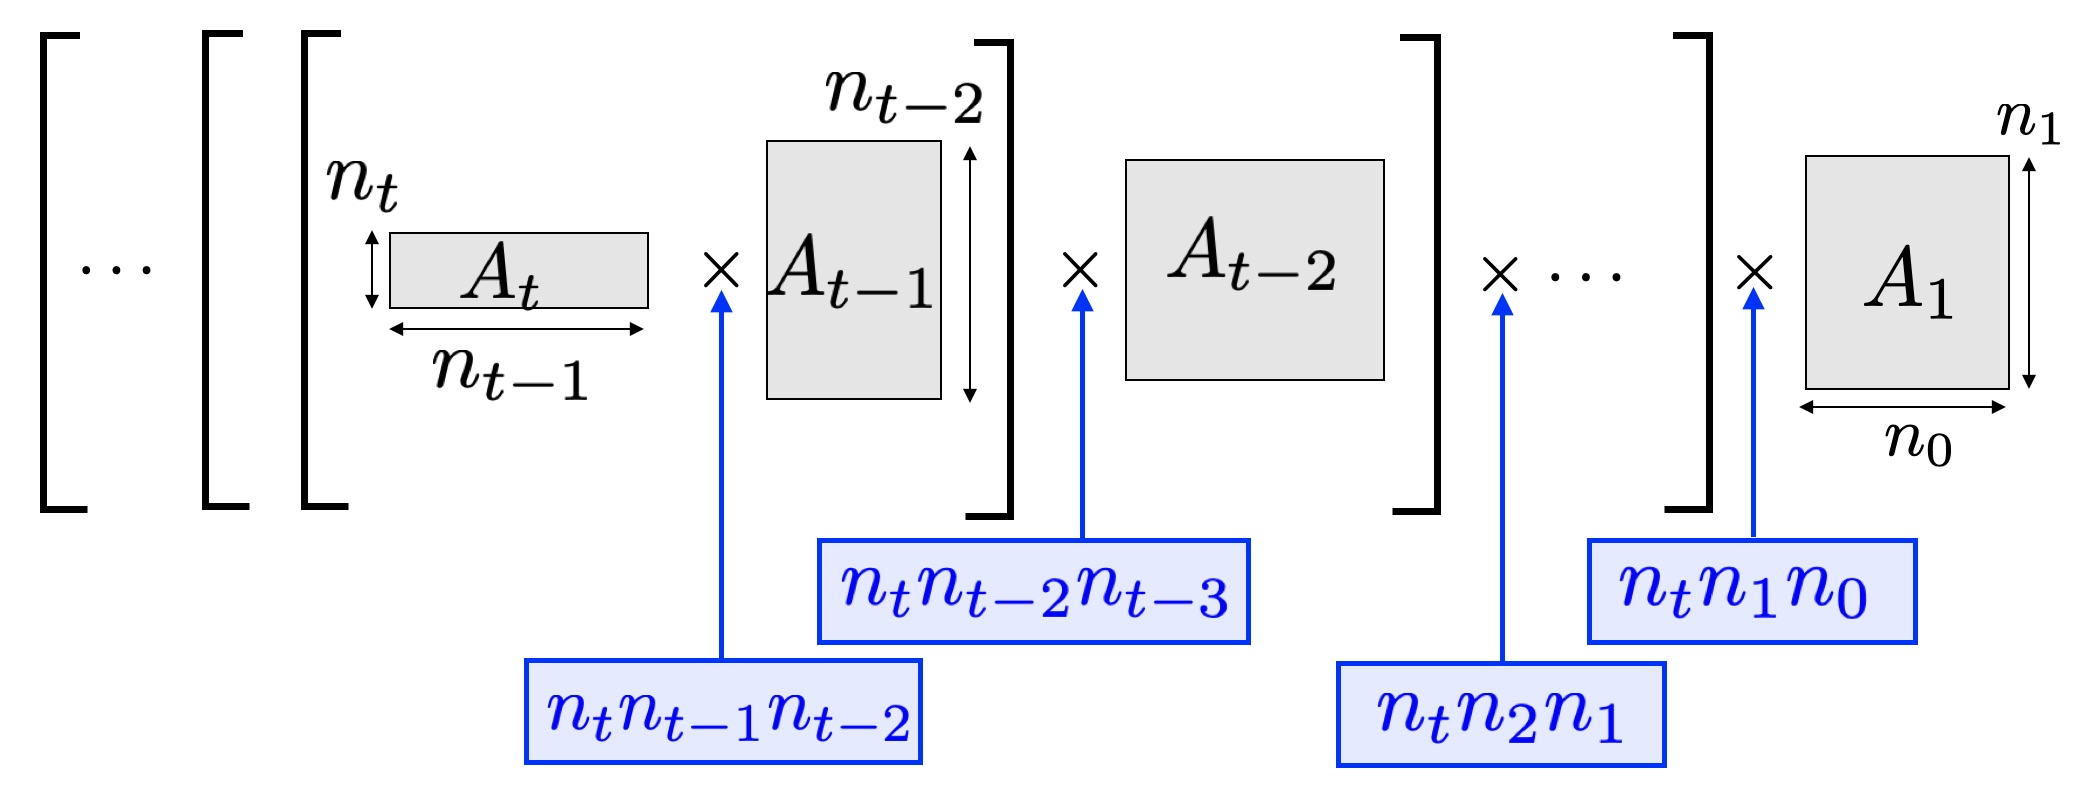
\includegraphics[width=.45\linewidth]{auto-diff/matrix-backward} 
\caption{\label{fig-matrix-mult}
Complexity of forward (left) and backward (right) modes for composition of functions. 
}
\end{figure}

We note that the computation of the product $A \times B$ of $A \in \RR^{n \times p}$ with $B \in \RR^{p \times q}$ necessitates $npq$ operations.
%
As shown on Figure~\ref{fig-matrix-mult}, the complexity of the forward and backward modes are
\eq{
	n_0 \sum_{k=1}^{t-1} n_k n_{k+1}
	\qandq
	n_t \sum_{k=0}^{t-2} n_k n_{k+1}
}
So if $n_t \ll n_0$ (which is the typical case in ML scenario where $n_t=1$) then the backward mode is cheaper. 


%%%%%%%%%%%%%%%%%%%%%%%%%%%%%%%%%%%%%%%%%%%%%%%%%%%%%%%%%%%%%%%%%%%%%%%%
\subsection{Feed-forward Architecture}

We can generalize the previous example to account for feed-forward architectures, such as neural networks, which are of the form
\eql{\label{eq-feednets}
	\foralls k=1, \ldots, t, \quad x_{k} = f_k(x_{k-1},\th_{k-1})
}
where $\th_{k-1}$ is a vector of parameters and $x_0 \in \RR^{n_0}$ is given. The function to minimize has the form
\eql{\label{eq-loss-feedf}
	f(\th) \eqdef L(x_t)
}
where $L : \RR^{n_t} \rightarrow \RR$ is some loss function (for instance a least square or logistic prediction risk) and $\th=(\th_k)_{k=0}^{t-1}$. Figure~\ref{fig-mlp}, top, displays the associated computational graph.


\begin{figure}
\centering
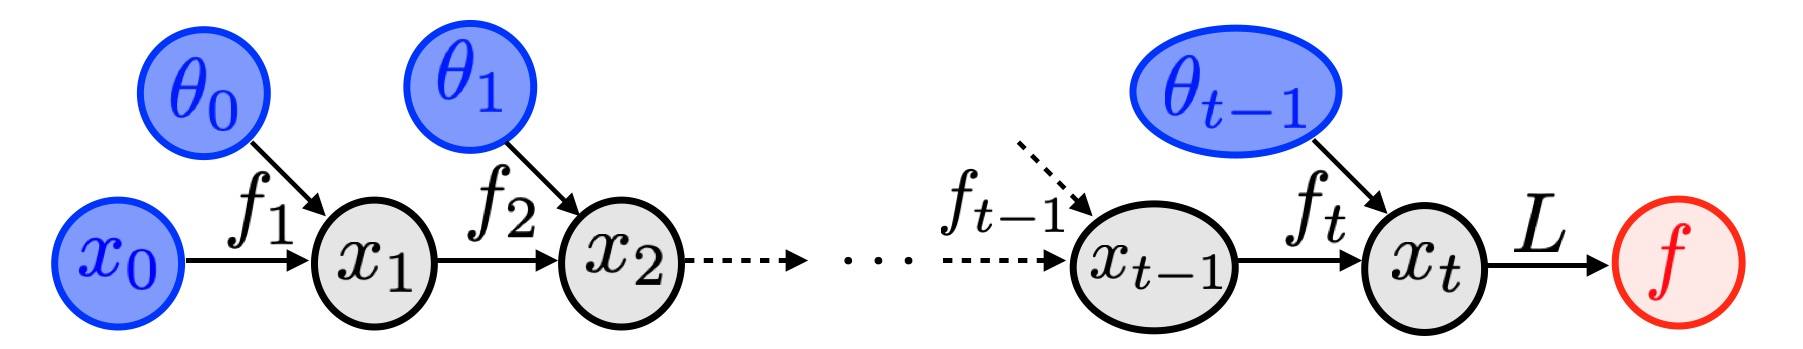
\includegraphics[width=.7\linewidth]{auto-diff/archi-feedforward} 
\caption{\label{fig-mlp}
Computational graph for a feedforward architecture.
}
\end{figure}


One can use the reverse mode automatic differentiation to compute the gradient of $f$ by computing successively the gradient with respect to all $(x_k,\th_k)$. One initializes
\eq{
	\nabla_{x_t} f = \nabla L(x_t) 	
}
and then recurse from $k=t-1$ to $0$
\eql{\label{eq-backprop-discr}
	z_{k-1} = [\partial_x f_k(x_{k-1},\th_{k-1})]^\top z_k
	\qandq
	\nabla_{\th_{k-1}} f = [\partial_\th f_k(x_{k-1},\th_{k-1})]^\top (\nabla_{x_{k}} f)
}
where we denoted $z_k \eqdef \nabla_{x_{k}} f(\th)$ the gradient with respect to $x_{k}$.

%%%
\paragraph{Multilayers perceptron.}

For instance, feedforward deep network (fully connected for simplicity) corresponds to using 
\eql{\label{eq-mlp-func}
	\foralls x_{k-1} \in \RR^{n_{k-1}}, \quad
	f_k(x_{k-1},\th_{k-1}) = \rho( \th_{k-1} x_{k-1} )
} 
where $\th_{k-1} \in \RR^{n_{k} \times n_{k-1}}$ are the neuron's weights and $\rho$ a fixed pointwise linearity, see Figure~\ref{fig-mlp-param}.
%
One has, for a vector $z_k \in \RR^{n_k}$ (typically equal to $\nabla_{x_{k}} f$)
\eq{
	\left\{
	\begin{matrix}
	[\partial_x f_k(x_{k-1},\th_{k-1})]^\top (z_k) = \th_{k-1}^\top w_k z_k, \\
	[\partial_\th f_k(x_{k-1},\th_{k-1})]^\top (z_k) = w_k x_{k-1}^\top
	\end{matrix}
	\right.
	\qwhereq
	w_k \eqdef \diag(\rho'(\th_{k-1} x_{k-1})).
}

\begin{figure}
\centering
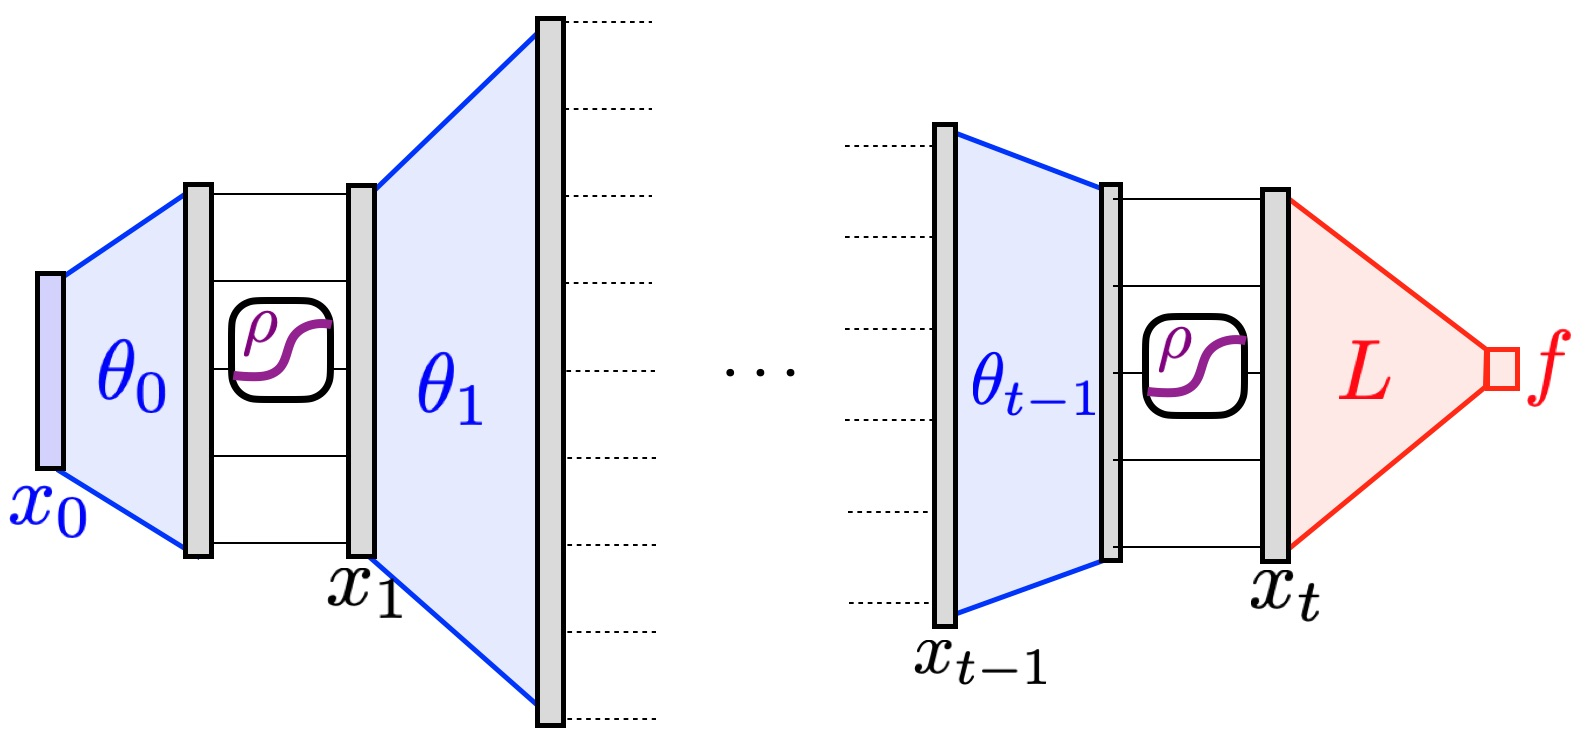
\includegraphics[width=.6\linewidth]{auto-diff/network-mlp} 
\caption{\label{fig-mlp-param}
Multi-layer perceptron parameterization.
}
\end{figure}



%%%
\paragraph{Link with adjoint state method.}

One can interpret~\eqref{eq-feednets} as a time discretization of a continuous ODE. 
%
One imposes that the dimension $n_k=n$ is fixed, and denotes $x(t) \in \RR^n$ a continuous time evolution, so that $x_{k} \rightarrow x(k \tau)$ when $k \rightarrow +\infty$ and $k \tau \rightarrow t$. 
%
Imposing then the structure
\eql{\label{eq-flow-eq}
	f_k(x_{k-1},\th_{k-1}) = x_{k-1} + \tau u(x_{k-1},\th_{k-1}, k\tau)
}
where $u(x,\th,t) \in \RR^n$ is a parameterized vector field, as $\tau \rightarrow 0$, one obtains the non-linear ODE
\eql{\label{eq-ode-structure}
	\dot x(t) = u(x(t),\th(t),t)
}
with $x(t=0)=x_0$.

Denoting $z(t) = \nabla_{x(t)} f(\th)$ the ``adjoint'' vector field, the discrete equations~\eqref{eq-backprop-discr} becomes the so-called adjoint equations, which is a linear ODE 
\eq{
	\dot z(t)  =  - [\partial_x u(x(t),\th(t),t)]^\top z(t)
	\qandq
	\nabla_{\th(t)} f(\th) = [\partial_\th u(x(t),\th(t),t)]^\top z(t).
}
Note that the correct normalization is $\frac{1}{\tau} \nabla_{\th_{k-1}} f  \rightarrow \nabla_{\th(t)} f(\th)$

%%%%%%%%%%%%%%%%%%%%%%%%%%%%%%%%%%%%%%%%%%%%%%%%%%%
\subsection{Recurrent Architectures}

Parametric recurrent functions are obtained by using the same parameter $\th=\th_k$ and $f_k=h$ recursively in~\eqref{eq-mlp-func}, so that 
\eql{\label{eq-feednets-recur}
	\foralls k=1, \ldots, t, \quad x_{k} = h(x_{k-1},\th).
}
We consider a real valued function of the form
\eq{
	f(\th) = L(x_t,\th)
}
so that here the final loss depends on $\th$ (which is thus more general than~\eqref{eq-loss-feedf}).  Figure~\ref{fig-recur}, bottom, displays the associated computational graph.


\begin{figure}
\centering
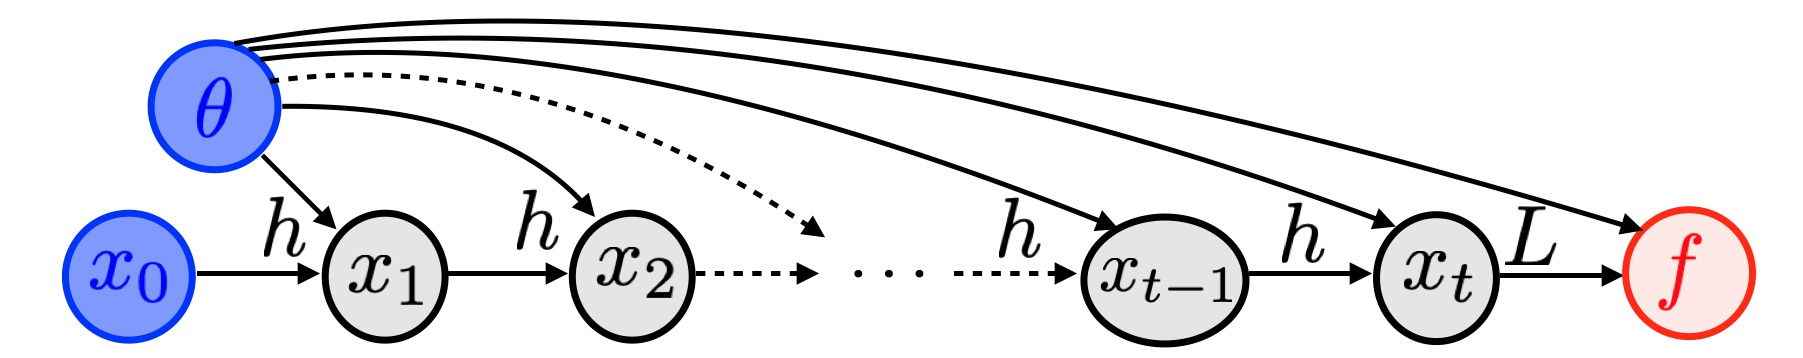
\includegraphics[width=.6\linewidth]{auto-diff/archi-recurrent}
\caption{\label{fig-recur}
Computational graph for a recurrent architecture.
}
\end{figure}

The back-propagation then operates as 
\eql{\label{eq-backprop-discr}
	\nabla_{x_{k-1}} f = [\partial_x h(x_{k-1},\th)]^\top \nabla_{x_{k}} f
	\qandq
	\nabla_{\th} f = 
		\nabla_\th L(x_t,\th) + 
		\sum_k [\partial_\th h(x_{k-1},\th)]^\top \nabla_{x_{k}} f.
}
Similarly, writing $h(x,\th) = x + \tau u(x,\th)$, letting $(k,k\tau) \rightarrow (+\infty,t)$, one obtains the forward non-linear ODE with a time-stationary vector field
\eq{
	\dot x(t) = u(x(t),\th)
}
and the following linear backward adjoint equation, for $f(\th)=L(x(T),\th)$
\eql{\label{eq-jacobian-mlp}
	\dot z(t)  =  - [\partial_x u(x(t),\th)]^\top z(t)
	\qandq
	\nabla_{\th} f(\th) = \nabla_\th L(x(T),\th) + \int_0^T [\partial_\th f(x(t),\th)]^\top z(t) \d t.
}
with $z(0) = \nabla_x L(x_t,\th)$. 

%%%%%
\paragraph{Residual recurrent networks. }

A recurrent network is defined using
\eq{
	h(x,\th) = x + W_2^\top \rho( W_1 x )
}
as displayed on Figure~\ref{fig-recurrent-param}, where $\th = (W_1, W_2) \in (\RR^{n \times q})^2$ are the weights and $\rho$ is a pointwise non-linearity. The number $q$ of hidden neurons can be increased to approximate more complex functions. 
%
In the special case where $W_2=- \tau W_1$, and $\rho=\psi'$, then this is a special case of an argmin layer~\eqref{eq-argmin-layer} to minimize the function $\Ee(x,\th) = \psi( W_1 x )$ using gradient descent, where $\psi(u)=\sum_i \psi(u_i)$ is a separable function.
%
The Jacobians $\partial_\th h$ and $\partial_x h$ are computed similarly to~\eqref{eq-jacobian-mlp}.

\begin{figure}
\centering
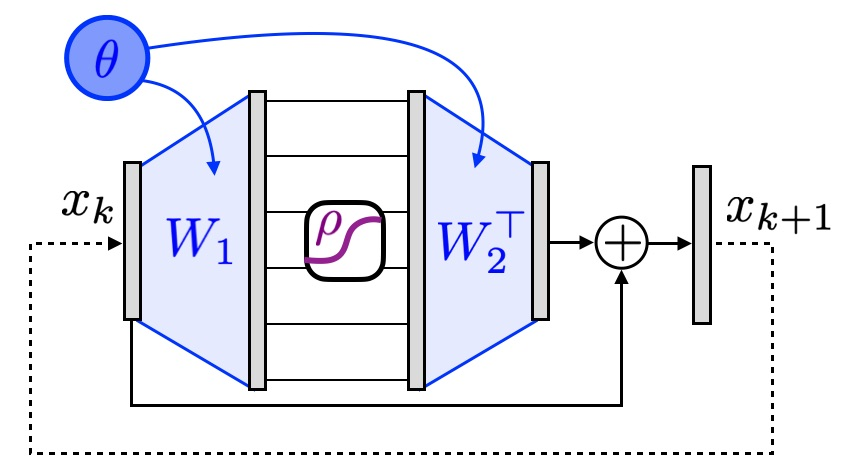
\includegraphics[width=.5\linewidth]{auto-diff/network-recur} 
\caption{\label{fig-recurrent-param}
Recurrent residual perceptron parameterization.
}
\end{figure}


%%%%%
\paragraph{Mitigating memory requirement. }

The main issue of applying this backpropagation method to compute $\nabla f(\th)$ is that it requires a large memory to store all the iterates $(x_k)_{k=0}^t$. A workaround is to use checkpointing, which stores some of these intermediate results and re-run partially the forward algorithm to reconstruct missing values during the backward pass. Clever hierarchical method perform this recursively in order to only require $\log(t)$ stored values and a $\log(t)$ increase on the numerical complexity. 

In some situation, it is possible to avoid the storage of the forward result, if one assume that the algorithm can be run backward. This means that there exists some functions $g_k$ so that 
\eq{
	x_{k} = g_k(x_{k+1},\ldots,x_t).
}
In practice, this function typically also depends on a few extra variables, in particular on the input values $(x_0,\ldots,x_s)$.

An example of this situation is when one can split the (continuous time) variable as $x(t)=(r(t),s(t))$ and the vector field $u$ in the continuous ODE~\eqref{eq-ode-structure} has a symplectic structure of the form $u((r,s),\th,t) = ( F(s,\th,t),G(r,\th,t) )$. One can then use a leapfrog integration scheme, which defines  
\eq{
	r_{k+1} = r_k + \tau F(s_k,\th_k,\tau k)
	\qandq
	s_{k+1} = s_k + \tau G(r_{k+1},\th_{k+1/2},\tau (k+1/2)).
}
One can reverse these equation exactly as
\eq{
	s_k = s_{k+1} - \tau G(r_{k+1},\th_{k+1/2},\tau (k+1/2)).
	\qandq
	r_k = r_{k+1}  - \tau F(s_k,\th_k,\tau k). 
}

%%%%%
\paragraph{Fixed point maps}

In some applications (some of which are detailed below), the iterations $x_k$ converges to some $x^\star(\th)$ which is thus a fixed point 
\eq{
	x^\star(\th) = h(x^\star(\th),\th). 
}
Instead of applying the back-propagation to compute the gradient of $f(\th) = L(x_t,\th)$, one can thus apply the implicit function theorem to compute the gradient of $f^\star(\th) = L(x^\star(\th),\th)$. Indeed, one has
\eql{\label{eq-impl-func-formula}
	\nabla f^\star(\th) = [\partial x^\star(\th)]^\top( \nabla_x L(x^\star(\th),\th) )
		 + \nabla_\th L(x^\star(\th),\th).
}
Using the implicit function theorem one can compute the Jacobian as
\eq{
	\partial x^\star(\th) =  - \pa{  \pd{h}{x}(x^\star(\th),\th) }^{-1}  \pd{h}{\th}(x^\star(\th),\th). 
}
In practice, one replace in these formulas $x^\star(\th)$ by $x_t$, which produces an approximation of $\nabla f(\th)$. 
%
The disadvantage of this method is that it requires the resolution of a linear system, but its advantage is that it bypass the memory storage issue of the backpropagation algorithm.



%%%%%
\paragraph{Argmin layers}

One can define a mapping from some parameter $\th$ to a point $x(\th)$ by solving a parametric optimization problem
\eq{
	x(\th) = \uargmin{x} \Ee(x,\th).
}
The simplest approach to solve this problem is to use a gradient descent scheme, $x_0=0$ and
\eql{\label{eq-argmin-layer}
	x_{k+1} = x_k - \tau \nabla \Ee(x_k,\th). 
}
This has the form~\eqref{eq-flow-eq} when using the vector field $u(x,\th) = \nabla \Ee(x_k,\th)$. 

Using formula~\eqref{eq-impl-func-formula} in this case where $h=\nabla \Ee$, one obtains
\eq{
	\nabla f^\star(\th) = -\pa{ \frac{\partial^2 \Ee}{\partial x \partial \th}(x^\star(\th),\th) }^\top 
		\pa{  \pdd{\Ee}{x}(x^\star(\th),\th) }^{-1}
		( \nabla_x L(x^\star(\th),\th) )
		 + \nabla_\th L(x^\star(\th),\th)
}

In the special case where the function $f(\th)$ is the minimized function itself, i.e. $f(\th)=\Ee(x^\star(\th),\th)$, i.e. $L=\Ee$, then one can apply the implicit function theorem formula~\eqref{eq-impl-func-formula}, which is much simpler since in this case $\nabla_x L(x^\star(\th),\th)=0$ so that 
\eql{\label{eq-danskin}
	\nabla f^\star(\th) = \nabla_\th L(x^\star(\th),\th). 
}
This result is often called Danskin theorem or the envelope theorem. 


%%%%%
\paragraph{Sinkhorn's algorithm}

Sinkhorn algorithm approximates the optimal distance between two histograms $a \in \RR^n$ and $b \in \RR^m$ using the following recursion on multipliers, initialized as $x_0 \eqdef (u_0,v_0) = (1_n,1_m)$
\eq{
	u_{k+1} = \frac{a}{K v_k}, \qandq
	v_{k+1} = \frac{b}{K^\top u_k}.
}
where $\frac{\cdot}{\cdot}$ is the pointwise division and $K \in \RR_+^{n \times m}$ is a kernel.
%
Denoting $\th=(a,b) \in \RR^{n+m}$ and $x_k=(u_k,v_k) \in \RR^{n+m}$, the OT distance is then approximately equal to 
\eq{
	f(\th) = \Ee(x_t,\th) \eqdef \dotp{a}{\log(u_t)} + \dotp{b}{\log(v_t)} - \epsilon \dotp{K u_t}{v_t}. 
}
Sinkhorn iteration are alternate minimization to find a minimizer of $\Ee$. 

Denoting  $\Kk \eqdef \begin{pmatrix} 0 & K \\ K^\top & 0 \end{pmatrix} \in \RR^{(n+m) \times (n+m)}$, one can re-write these iterations in the form~\eqref{eq-feednets-recur} using 
\eq{
	h(x,\th) = \frac{\th}{\Kk x}
	\qandq
	L(x_t,\th) = \Ee(x_t,\th)  = \dotp{\th}{\log(x_t)} - \epsilon \dotp{K u_t}{v_t}. 
}
One has the following differential operator 
\eq{
	[\partial_x h(x,\th)]^\top = -\Kk^\top \diag\pa{\frac{\th}{(\Kk x)^2}}, \quad
	[\partial_\th h(x,\th)]^\top = \diag\pa{\frac{1}{\Kk x}}.
}
%\eq{
%	\nabla_x L(x,\th) = ??, \quad
%	\nabla_\th L(x,\th) = ??. 
%}
Similarly as for the argmin layer, at convergence $x_k \rightarrow x^\star(\th)$, one finds a minimizer of $\Ee$, so that $\nabla_x L(x^\star(\th),\th)=0$ and thus the gradient of $f^\star(\th)=\Ee(x^\star(\th),\th)$ can be computed using~\eqref{eq-danskin} i.e.
\eq{
	\nabla f^\star(\th) = \log(x^\star(\th)).
}






% % !TEX root = ../CourseOT.tex

%%%%%%%%%%%%%%%%%%%%%%%%%%%%%%%%%%%%%%%%%%%%%%%%%%%%%%%%%%%%%%%%%%%%%%%%%%%
%%%%%%%%%%%%%%%%%%%%%%%%%%%%%%%%%%%%%%%%%%%%%%%%%%%%%%%%%%%%%%%%%%%%%%%%%%%
%%%%%%%%%%%%%%%%%%%%%%%%%%%%%%%%%%%%%%%%%%%%%%%%%%%%%%%%%%%%%%%%%%%%%%%%%%%
\section{Optimal Matching between Point Clouds}

%%%%%%%%%%%%%%%%%%%%%%%%%%%%%%%%%%%%%%%%%%%%%%%%%%%%%%%%%%%%%%%%%%%%%%%%%%%
\subsection{Monge Problem between Discrete points}
\label{sec-monge-pbm}

%%%%%%%
\paragraph{Matching problem}

Given a cost matrix $(\C_{i,j})_{i \in \range{n}, j \in \range{m}}$, assuming $n=m$, the optimal assignment problem seeks for a bijection $\si$ in the set $\Perm(n)$ of permutations of $n$ elements solving
\eql{\label{eq-optimal-assignment}
	\umin{\si \in \Perm(n)} \frac{1}{n}\sum_{i=1}^n \C_{i,\si(i)}.
}
One could naively evaluate the cost function above using all permutations in the set $\Perm(n)$. However, that set has size $n!$, which is gigantic even for small $n$. 
% Consider for instance that such a set has more than $10^{100}$ elements~\cite{Dantzig1983} when $n$ is as small as 70. That problem can therefore only be solved if there exist efficient algorithms to optimize that cost function over the set of permutations, which will be the subject of~\S\ref{s-matching}.
In general the optimal $\si$ is non-unique. 

% \begin{rem}[Uniqueness] Note that the optimal assignment problem may have several optimal solutions. Suppose for instance that $n=m=2$ and that the matrix $\C$ is the pairwise distance matrix between the 4 corners of a 2-dimensional square of side length $1$, as represented in the left plot in Figure~\ref{fig-non-unique-matching}. In that case only two assignments exist, and they share the same cost. \end{rem}

%\begin{figure}
%\centering
%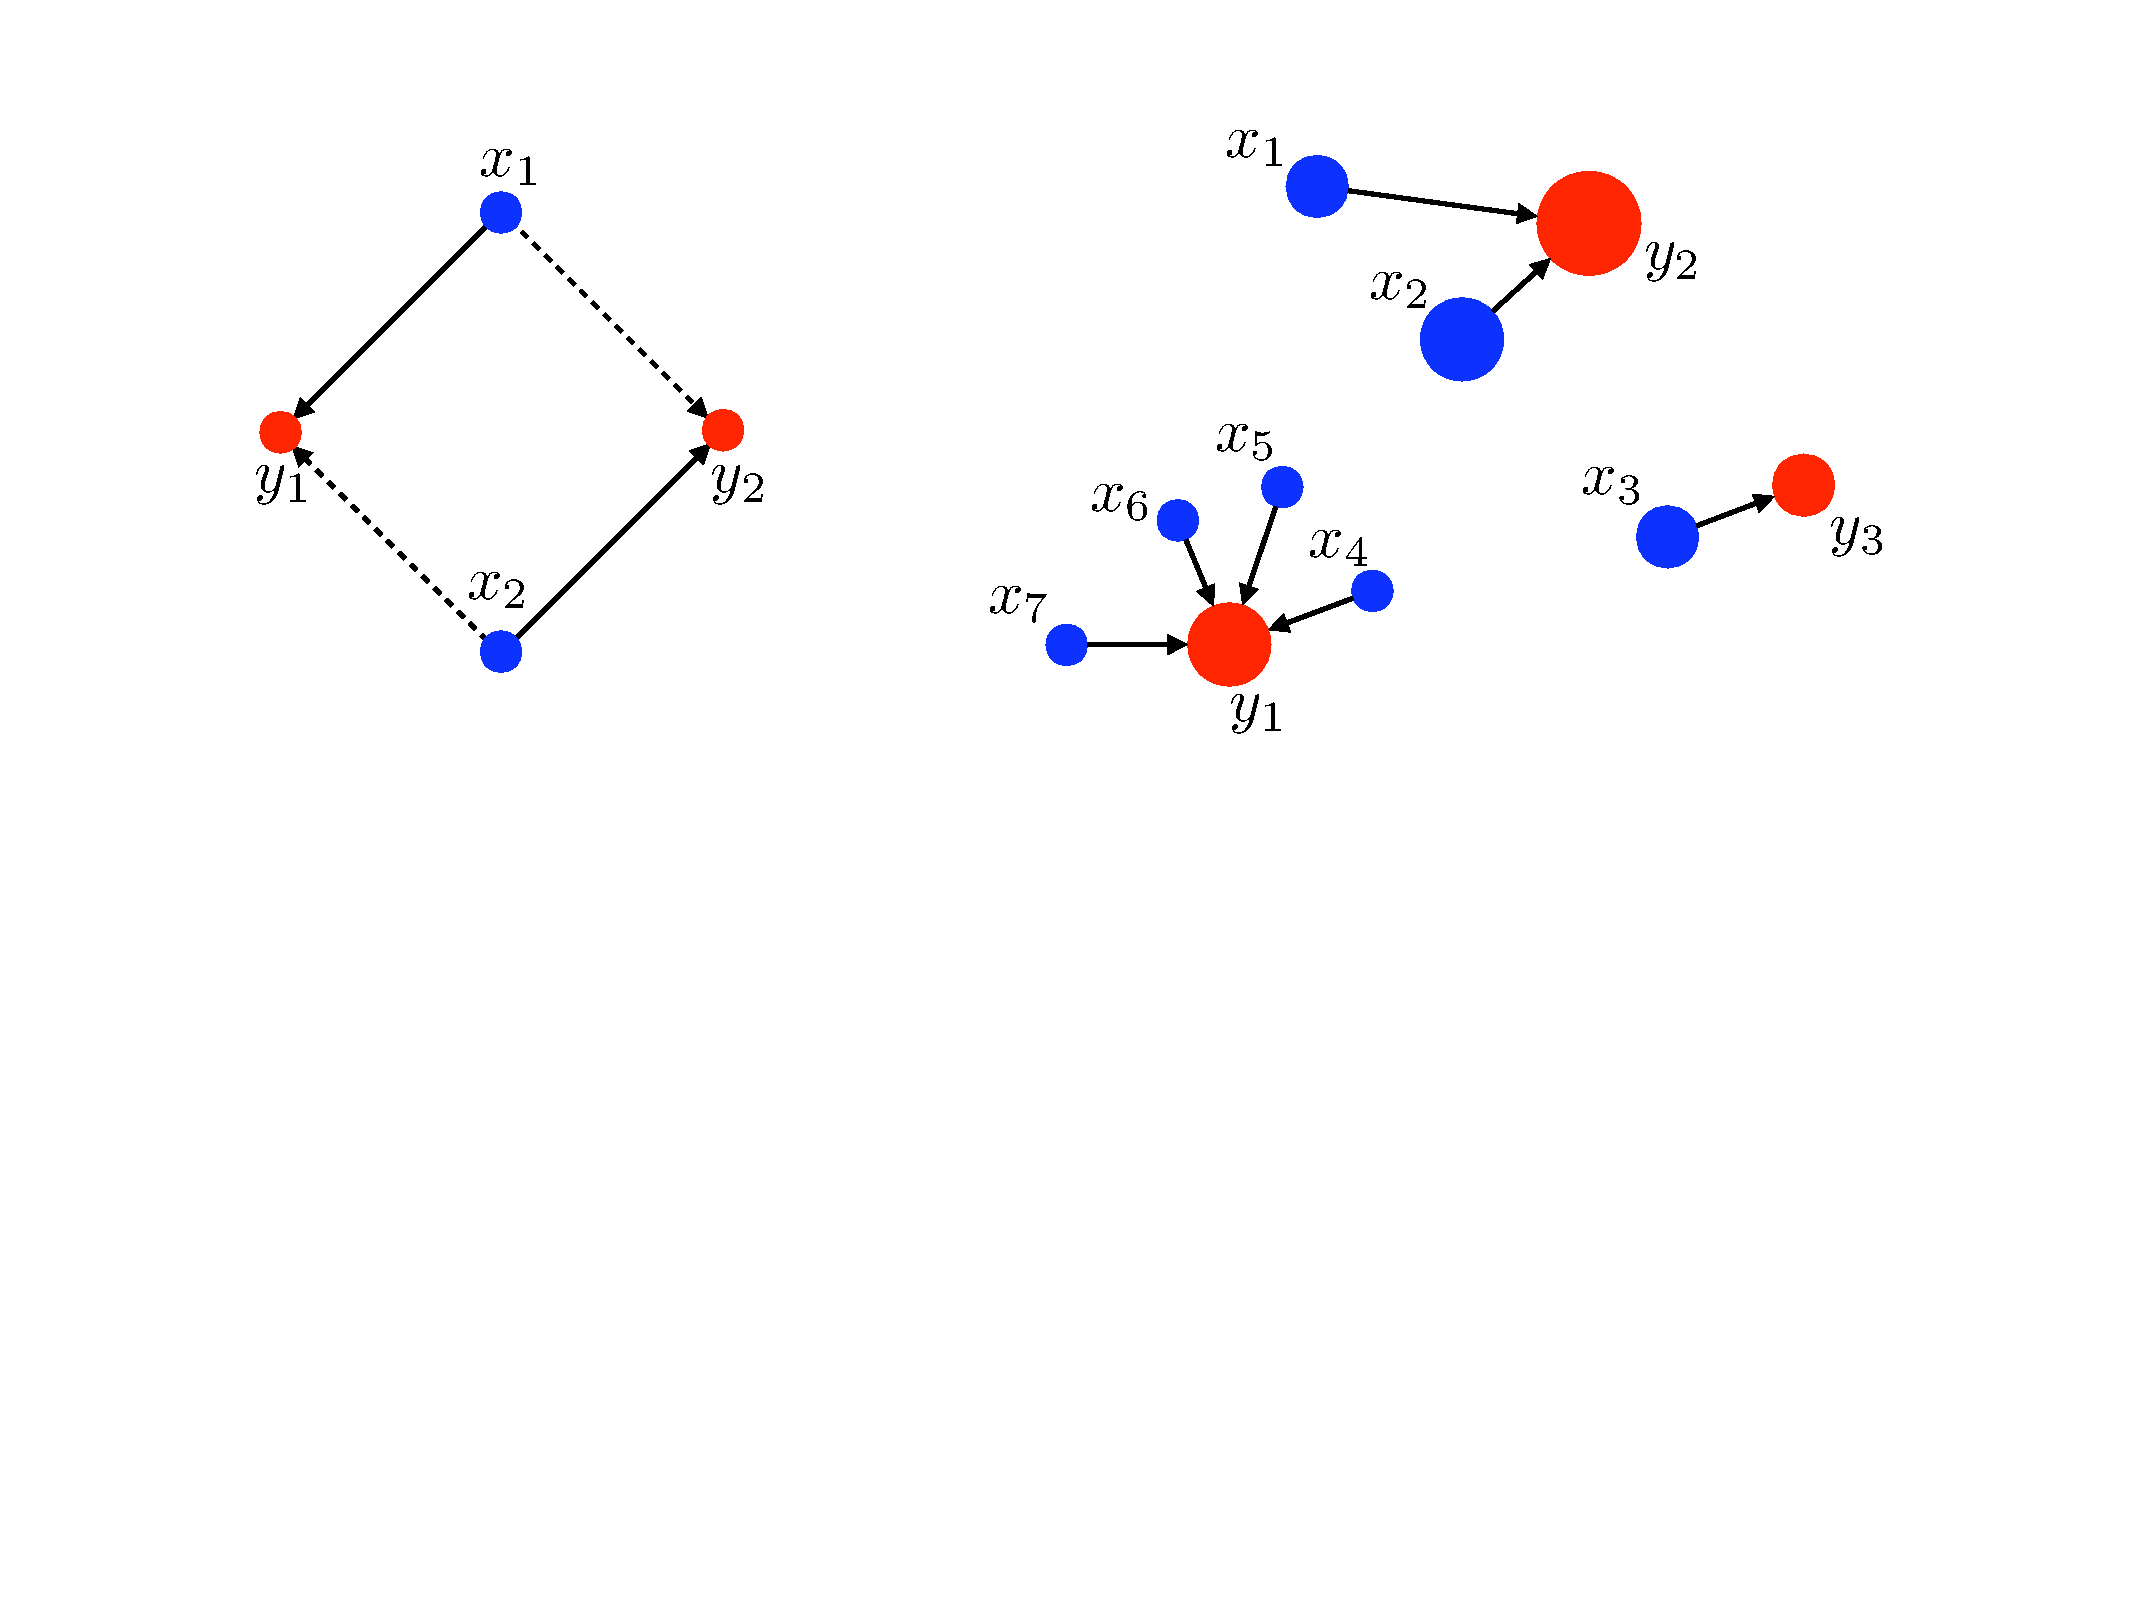
\includegraphics[width=.5\linewidth]{non-unique-optimal-matching/non-unique-optimal-matching}
%\caption{\label{fig-non-unique-matching}
%(left) blue dots from measure $\alpha$ and red dots from measure $\beta$ are pairwise equidistant. Hence, either matching $\sigma=(1,2)$ (full line) or $\sigma=(2,1)$ (dotted line) is optimal. (right) a Monge map can associate the blue measure $\alpha$ to the red measure $\beta$. The weights $\alpha_i$ are displayed proportionally to the area of the disk marked at each location. The mapping here is such that $T(x_1)=T(x_2)=y_2$, $T(x_3)=y_3$, whereas for $4\leq i\leq 7$ we have $T(x_i)=y_1$.
%}
%\end{figure}


\paragraph{1D case}

If the cost is of the form $\C_{i,j}=h(x_i-y_j)$, where $h: \RR \rightarrow \RR^+$ is  convex (for instance $\C_{i,j}=|x_i-y_j|^p$ for $p \geq 1$), one has that an optimal $\si$ necessarily defines an increasing map $x_i \mapsto x_{\si(i)}$, i.e. 
\eq{
	\foralls (i,j), \quad (x_i-y_j)(x_{\si(i)}-y_{\si(j)}) \geq 0.
}
Indeed, if this property is violated, i.e. there exists $(i,j)$ such that $(x_i-y_j)(x_{\si(i)}-y_{\si(j)}) < 0$, then one can defines a permutation $\tilde \si$ by swapping the match, i.e. $\tilde\si(i)=\si(j)$ and $\tilde\si(j)=\si(i)$, with a better cost
\eq{
	\sum_i h(x_{i}-y_{\tilde \si(i)}) \leq \sum_i h(x_{i}-y_{\si(i)}),  
}
because
\eq{
	h(x_{i}-y_{\si(j)}) + h(x_{j}-y_{\si(i)}) 
	\leq
	h(x_{i}-y_{\si(i)}) + h(x_{j}-y_{\si(j)}).  
}
So the algorithm to compute an optimal transport (actually all optimal transport) is to sort the points, i.e. find some pair of permutations $\si_X, \si_Y$ such that
\eq{
	x_{\si_X(1)} \leq \si_{\si_X(2)} \leq \ldots
	\qandq
	y_{\si_Y(1)} \leq \si_{\si_Y(2)} \leq \ldots
}
and then an optimal match is mapping $x_{\si_X(k)} \mapsto y_{\si_Y(k)}$, i.e. an optimal transport is $\si = \si_Y \circ \si_X^{-1}$. The total computational cost is thus $O(n\log(n))$ using for instance quicksort algorithm.
%
Note that if $\phi : \RR \rightarrow \RR$ is an increasing map, with a change of variable, one can apply this technique to cost of the form $h(|\phi(x)-\phi(y)|)$. 
%
A typical application is grayscale histogram equalization of the luminance of images. 

Note that is $h$ is concave instead of being convex, then the behavior is totally different, and the optimal match actually rather exchange the positions, and in this case there exists an $O(n^2)$ algorithm.   
% Note that in the case of concave cost of the distance, for instance when $p<1$, the behaviour of the optimal transport plan is very different, see~\cite{delon-concave}, which describes an efficient solver in this case.

%
%
%\begin{figure}
%\centering
%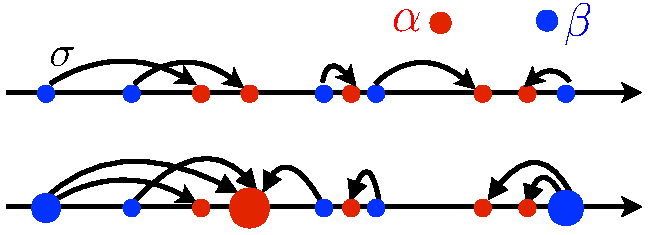
\includegraphics[width=.4\linewidth]{1d-discrete/1d-schematic}
%\caption{\label{fig-1d-discrete}
%1-D optimal couplings: each arrow $x_i \rightarrow y_j$ indicate a non-zero $\P_{i,j}$ in the optimal coupling.
%% 
%Top: empirical measures with same number of points (optimal matching).
%Bottom: generic case. 
%%
%This corresponds to monotone rearrangements, if $x_i \leq x_{i'}$ are such that $\P_{i,j} \neq 0, \P_{i',j'} \neq 0$, then necessarily $y_j \leq y_{j'}$.
%}
%\end{figure}


%%%%%%%%%%%%%%%%%%%%%%%%%%%%%%%%%%%%%%%%%%%%%%%%%%%%%%%%%%%%%%%%%%%%%%%%%%%
\subsection{Matching Algorithms}

There exists efficient algorithms to solve the optimal matching problems. The most well known are the hungarian and the auction algorithm, which runs in $O(n^3)$ operations. Their derivation and analysis is however very much simplified by introducing the Kantorovitch relaxation and its associated dual problem.
%
A typical application of these methods is the equalization of the color palette between images, which corresponds to a 3-D optimal transport. 

  
  
  



% \nocite{*}

\bibliographystyle{plain}
\bibliography{all}

\end{document}
